\documentclass[
    twoside,         % oneside/twoside : Einseitiger oder zweiseitiger Druck?
    12pt,            % Bezug: 12-Punkt Schriftgre
    DIV15,           % Randaufteilung, siehe Dokumentation "KOMA"-Script
    BCOR17mm,        % Bindekorrektur: Innen 17mm Platz lassen. Copyshop-getestet.
    headsepline,     % Unter Kopfzeile Trennlinie (aus: headnosepline)
    footsepline,     % ber Fuzeile Trennlinie (aus: footnosepline)
    openright,       % Neue Kapitel im zweiseitigen Druck rechts beginnen lassen
    a4paper,         % Seitenformat A4
    abstracton,      % Abstract einbinden
    english,
    listof=totoc,version=first,      % Div. Verzeichnisse ins Inhaltsverzeichnis aufnehmen
    bibliography=totoc,version=first,        % Literaturverzeichnis ins Inhaltsverzeichnis aufnehmen
    titlepage,       % Titelseite aktivieren
    headinclude,     % Seiten-Head in die Satzspiegelberechnung mit einbeziehen
    footexclude,     % Seiten-Foot nicht in die Satzspiegelberechnung mit einbeziehen
    numbers=noenddot,version=first % Gliederungsnummern ohne abschlieenden Punkt darstellen
] {scrreprt}       % Dokumentenstil: "Report" aus dem KOMA-Skript-Paket

\usepackage[active]{srcltx}
%\usepackage[activate=normal]{pdfcprot\documentclass[options]{class}} % Optischer Randausgleich -> pdflatex!
\usepackage{ifthen}
\usepackage[english,vietnamese]{babel}
%\usepackage[fixlanguage]{babelbib}
%\setbiblanguage{english}
\usepackage[utf8]{inputenc}
% \usepackage[latin1]{inputenc}
\usepackage[T5,T1]{fontenc}
\usepackage{fontawesome5}
\usepackage[T1]{url}
\usepackage{ae}
\usepackage[final]{graphicx}
\usepackage[automark]{scrlayer-scrpage}
\usepackage{setspace}
\usepackage{subcaption}
\usepackage{floatflt} 
\usepackage{rotating} 
\usepackage{wrapfig}
%\usepackage{subfig}
\usepackage{graphicx}
%\usepackage[first,light]{draftcopy} % Fr Probedruck
\usepackage{lineno}
\usepackage[plainpages=false,pdfpagelabels,hypertexnames=false]{hyperref}
\usepackage{pdfpages} %include pdf files
\usepackage{listings} %include sourcecode
\usepackage{color}
\usepackage{multirow}
\usepackage{verbatim}
\usepackage{amsmath}
\usepackage{amssymb}
\usepackage{amsfonts}
\usepackage{bbm}
\usepackage{enumitem}
\usepackage{array}
\usepackage{nomencl}
\usepackage{xcolor}
\usepackage{xfrac}
\usepackage{longtable}
\usepackage{url}
\usepackage{subcaption}
%\usepackage{paralist}
\usepackage{tipa}
\usepackage{csquotes}
%\usepackage{textcomp}  %mit \textcent geht Cent-Symbol
\usepackage{diagbox}
\usepackage[linesnumbered,ruled]{algorithm2e}
\usepackage{geometry}
\geometry{
    a4paper,
    % total={170mm,257mm},
    left=35mm,
    right=25mm,
    top=20mm,
    bottom=25mm,
}


% Tiefe der Kapitelnummerierung beeinflussen
\setcounter{secnumdepth}{3} % Tiefe der Nummerierung
\setcounter{tocdepth}{3}    % Tiefe des Inhaltsverzeichnisses

% Hier in die zweite geschweifte Klammer jeweils
% die persnlichen Daten eintragen:
\newcommand{\typeofelaboration}{Master Thesis}
\newcommand{\nameofauthor}{Nguyễn Tiến Nam}
\newcommand{\emailofauthor}{hnhat.tran@gmail.com}
\newcommand{\idofauthor}{}
\newcommand{\majorofauthor}{Control Engineering and Automation}

\newcommand*\en{\fontencoding{T1}\selectfont\selectlanguage{english}}
\newcommand*\vn{\fontencoding{T5}\selectfont\selectlanguage{vietnamese}}
\makeatletter
\newcommand{\capitalize}[1]{%
    \edef\@tempa{\expandafter\@gobble\string#1}%
    \edef\@tempb{\expandafter\@car\@tempa\@nil}%
    \edef\@tempa{\expandafter\@cdr\@tempa\@nil}%
    \uppercase\expandafter{\expandafter\def\expandafter\@tempb\expandafter{\@tempb}}%
    \@namedef{\@tempb\@tempa}{\expandafter\MakeUppercase\expandafter{#1}}
}
\makeatother

\newcommand{\markup}[1]{\textbf{#1}}
\newcommand{\github}[1]{\href{#1}{\faGithubSquare\ \textit{#1}}}

% Seitenlayout festlegen. Hier nichts ndern!
\pagestyle{scrplain}
\ihead[]{\scriptsize \headmark}
\ohead[]{\scriptsize \typeofelaboration}
\chead[]{}
% \ifoot[]{\scriptsize \nameofauthor\ - \idofauthor}
\ifoot[]{\scriptsize \nameofauthor}
\ofoot[]{\pagemark}
\cfoot[]{}
\newcommand{\resethead}{\newpage%
    \ihead[]{\scriptsize \headmark}%
    \ohead[]{\scriptsize \typeofelaboration}%
    \chead[]{}%
}
\newcommand{\resetfoot}{\newpage%
    \ifoot[]{\scriptsize \nameofauthor\ - \idofauthor}%
    \ofoot[]{\pagemark}%
    \cfoot[]{}%
}
\renewcommand{\titlepagestyle}{scrheadings}
\renewcommand{\partpagestyle}{scrheadings}
\renewcommand{\chapterpagestyle}{scrheadings}
\renewcommand{\indexpagestyle}{scrheadings}

% Abschnittsweise Nummerierung anstatt fortlaufend. Hier nichts ndern!
\makeatletter
\@addtoreset{equation}{chapter}
\@addtoreset{figure}{chapter}
\@addtoreset{table}{chapter}
\renewcommand\theequation{\thechapter.\@arabic\c@equation}
\renewcommand\thefigure{\thechapter.\@arabic\c@figure}
\renewcommand\thetable{\thechapter.\@arabic\c@table}\makeatother


% Quelltextrahmen, klein. Hier nichts ndern!
\newsavebox{\inhaltkl}
\def\rahmenkl{\sbox{\inhaltkl}\bgroup\small\renewcommand{\baselinestretch}{1}\vbox\bgroup\hsize\textwidth}
\def\endrahmenkl{\par\vskip-\lastskip\egroup\egroup\fboxsep3mm%
\framebox[\textwidth][l]{\usebox{\inhaltkl}}}

% Quelltextrahmen, normale Groesse. Hier nichts ndern!
\newsavebox{\inhalt}
\def\rahmen{\sbox{\inhalt}\bgroup\renewcommand{\baselinestretch}{1}\vbox\bgroup\hsize\textwidth}
\def\endrahmen{\par\vskip-\lastskip\egroup\egroup\fboxsep3mm%
\framebox[\textwidth][l]{\usebox{\inhalt}}}


% Sonstige Befehlsdefinitionen hier ablegen.
\newcommand{\entspricht}{\stackrel{\wedge}{=}}
\definecolor{light-gray}{gray}{0.95}
\addto\captionsenglish{\renewcommand{\contentsname}{Table of Contents}}
%\makenomenclature
\makeglossary
\DeclareMathOperator*{\argmin}{argmin}
\DeclareMathOperator*{\argmax}{argmax}

\newcommand{\listofabbreviations}{%!TEX root = ../main.tex

\cleardoublepage
\ihead[]{\scriptsize{List of Abbreviations}}
\addcontentsline{toc}{chapter}{List of Abbreviations}
\chapter*{List of Abbreviations}

\begin{longtable}{p{.2\textwidth} p{.8\textwidth}}
    \textbf{ANN} & Artificial Neural Network\\
    \textbf{AP} & Average Pooling\\
    \textbf{CCA} & Canonical Correlation Analysis\\
    \textbf{CNN} & Convolutional Neural Network\\
    \textbf{DNN} & Deep Neural Network\\
    \textbf{GRU} & Gated Recurrent Unit\\
    \textbf{HAR} & Human Action Recognition\\
    \textbf{HoG} & Histogram of oriented Gradient\\
    \textbf{iDT} & improved Dense Trajectories\\
    \textbf{KCCA} & Kernel Canonical Correlation Analysis\\
    \textbf{kNN} & k-Neareast Neighbor\\
    \textbf{LDA} & Linear Discriminant Analysis\\
    \textbf{LSTM} & Long Short-Term Memory\\
    \textbf{MICA} & Multimedia, Information, Communication \& Applications International Research Institute\\
    \textbf{MLP} & Multilayer Perceptron\\
    \textbf{MST-AOG} & Multi-view Spatio-Temporal AND-OR Graph\\
    \textbf{MvA} & Multi-view Analysis\\
    \textbf{MvCCA} & Multi-view Canonical Correlation Analysis\\
    \textbf{MvCCDA} & Multi-view Common Component Discriminant Analysis\\
    \textbf{MvDA} & Multi-view Discriminant Analysis\\
    \textbf{MvDA-vc} & Multi-view Discriminant Analysis with View-Consistency\\
    \textbf{MvFDA} & Multi-view Fisher Discriminant Analysis\\
    \textbf{MvMDA} & Multi-view Modular Discriminant Analysis\\
    \textbf{MvML-LA} & Multi-view Manifold Learning with Locality Alignment\\
    \textbf{MvPLS} & Multi-view Partial Least Square\\
    \textbf{pc-LDA} & Pairwise-Covariance Linear Discriminant Analysis\\
    \textbf{pc-MvDA} & Pairwise-Covariance Multi-view Discriminant Analysis\\
    \textbf{RNN} & Recurrent Neural Network\\
    \textbf{SOTA} & State Of The Art\\
    \textbf{SSM} & Self Similarity Matrix\\
    \textbf{TA} & Temporal Attention\\
    % \textbf{SVM} & Support Vector Machine\\
\end{longtable}

\resethead
}
\bibliographystyle{IEEEbib}

\begin{document}

    \onehalfspacing
    \clubpenalty=10000
    \widowpenalty=10000
    \vn
    %!TEX root = ../main.tex

\begin{titlepage}
\thispagestyle{empty}
\begin{center}
\textbf{\large{Hanoi University of Science and Technology}} \\
% \large{School of Electrical Engineering}

\vspace{0.2cm}

\begin{figure}[htbp]
    \begin{center}
    
\includegraphics[width=0.2\textwidth]{figs/hust-logo.jpg}
    \end{center}
\end{figure}

\vspace{0.5cm}

\textbf{\Huge{Master Thesis}} \\
\vspace{1.2cm}
\textbf{\LARGE{Human Action Recognition using Deep Learning and Multi-view Discriminant Analysis}} \\

\vspace{1.0cm}

\textbf{\large{TRAN HOANG NHAT}} \\
\small{\emailofauthor} \\
\vspace{0.3cm}
\textbf{\large{\majorofauthor}} \\
\vspace{2.5cm}

\small
\renewcommand{\arraystretch}{1.5} 
\begin{tabular}{lll}
    % \textbf{Submitted by:} & & Tran Hoang Nhat\\
    % \textbf{Date \& place of birth:} & & December 28, 1996, Hanoi\\
    % \textbf{Submission date:} & & October 20, 2020 \\
    % & & \\
    \textbf{Advisor:} & & Assoc. Prof. Dr. Tran Thi Thanh Hai \\
    \textbf{Faculty:} & & School of Electronics and Telecommunications \\
\end{tabular}
%\begin{tabular}{lll}
%\textbf{Faculty Advisors:}  & & Advisor 1 \\ & & Advisor 2 \\ & & Advisor 3\\
% \end{tabular}
% \end{flushleft}

\vspace{\fill}
\textbf{\normalsize{Hanoi, 10/2020}}
\end{center}
\end{titlepage}


    \cleardoublepage
    \footnotesize
    \pagenumbering{roman}
    \pagestyle{scrheadings}

    \normalsize
    %!TEX root = ../main.tex

%\renewcommand{\abstractname}{Kurzfassung}
\begin{abstract}
    % \addcontentsline{toc}{chapter}{Abstract}
    % \chapter*{Abstract}

    Human action recognition (HAR) has many implications in robotic and medical applications.
    Invariance under different viewpoints is one of the most critical requirements for practical deployment as it affects many aspects of the information captured such as occlusion, posture, color, shading, motion and background.
    In this thesis, a novel framework that leverages successful deep features for action representation and multi-view analysis to accomplish robust HAR under viewpoint changes.
    Specifically, various deep learning techniques, from 2D CNNs to 3D CNNs are investigated to capture spatial and temporal characteristics of actions at each individual view.
    A common feature space is then constructed to keep view invariant features among extracted streams.
    This is carried out by learning a set of linear transformations that projects separated view features into a common dimension.
    To this end, Multi-view Discriminant Analysis (MvDA) is adopted.
    However, the original MvDA suffers from odd situations in which the most class-discrepant common space could not be found because its objective is overly concentrated on scattering classes from the global mean but unaware of distance between specific pairs of classes.
    Therefore, we introduce a pairwise-covariance maximizing extension of MvDA that takes extra-class discriminance into account, namely pc-MvDA.
    The novel model also differs in the way that is more favorable for training of high-dimensional multi-view data.
    Experimental results on three datasets (IXMAS, MuHAVI, MICAGes) show the effectiveness of the proposed method.


\end{abstract}


% \begin{otherlanguage}{ngerman}
% %\renewcommand{\abstractname}{Kurzfassung}
% %\newcommand{\dtabstract}{\hyphenpenalty=10000}
% %{\dtabstract
% \begin{abstract}
% Das Gebiet des Music Information Retrieval befasst sich mit der automatischen Analyse von musikalischen Charakteristika. Ein Aspekt, der bisher kaum erforscht wurde, ist dabei der gesungene Text. Auf der anderen Seite werden in der automatischen Spracherkennung viele Methoden für die automatische Analyse von Sprache entwickelt, jedoch selten für Gesang. Die vorliegende Arbeit untersucht die Anwendung von Methoden aus der Spracherkennung auf Gesang und beschreibt mögliche Anpassungen. Zudem werden Wege zur praktischen Anwendung dieser Ansätze aufgezeigt. Fünf Themen werden dabei betrachtet: Phonemerkennung, Sprachenidentifikation, Schlagwortsuche, Text-zu-Gesangs-Alignment und Suche von Texten anhand von gesungenen Anfragen.\\
% Das größte Hindernis bei fast allen dieser Themen ist die Erkennung von Phonemen aus Gesangsaufnahmen. Herkömmliche, auf Sprache trainierte Modelle, bieten keine guten Ergebnisse für Gesang. Das Trainieren von Modellen auf Gesang ist schwierig, da kaum annotierte Daten verfügbar sind. Diese Arbeit zeigt zwei Ansätze auf, um solche Daten zu generieren. Für den ersten wurden Sprachaufnahmen künstlich gesangsähnlicher gemacht. Für den zweiten wurden Texte automatisch zu einem vorhandenen Gesangsdatensatz zugeordnet. Die neuen Datensätze wurden zum Trainieren neuer Modelle genutzt, welche deutliche Verbesserungen gegenüber sprachbasierten Modellen bieten.\\
% Auf diesen verbesserten akustischen Modellen aufbauend wurden Algorithmen aus der Spracherkennung für die verschiedenen Aufgaben angepasst, entweder durch das Verbessern der Robustheit gegenüber Gesangscharakteristika oder durch das Ausnutzen von hilfreichen Besonderheiten von Gesang. Beispiele für die verbesserte Robustheit sind der Einsatz von Keyword-Filler-HMMs für die Schlagwortsuche, ein i-Vector-Ansatz für die Sprachenidentifikation sowie eine Methode für das Alignment und die Textsuche, die stark schwankende Phonemdauern nicht bestraft. Die Besonderheiten von Gesang werden auf verschiedene Weisen genutzt: So z.B. in einem Ansatz für die Sprachenidentifikation, der lange Aufnahmen benötigt; in einer Methode für die Schlagwortsuche, die bekannte Phonemdauern in Gesang mit einbezieht; und in einem Algorithmus für das Alignment und die Textsuche, der bekannte Phonemkonfusionen verwertet.
% \end{abstract}
% \end{otherlanguage}

    %!TEX root = ../main.tex

\cleardoublepage
\ihead[]{Acknowledgements}
%\ohead[]{\pagemark}

% \addcontentsline{toc}{chapter}{Acknowledgements}
% \chapter*{Acknowledgements}

\begin{center}
\textbf{Acknowledgements}
\end{center}

This thesis would not have been possible without the help of many people.
First of all, I would like to express my gratitude to my primary advisor, Prof. Tran Thi Thanh Hai, who guided me throughout this project.
I would like to thank Prof. Le Thi Lan and Prof. Vu Hai for giving me deep insight, valuable recommendations and brilliant idea.

I am grateful for my time spent at MICA International Research Institute, where I learnt a lot about research and enjoyed a very warm and friendly working atmosphere.
In particular, I wish to extend my special thanks to PhD candidate. Nguyen Hong Quan and Dr. Doan Huong Giang who directly supported me.

Finally, I wish to show my appreciation to all my friends and family members who helped me finalizing the project.

\resethead


    \footnotesize
    \tableofcontents
    \normalsize

    \cleardoublepage
    \pagenumbering{arabic}
    \listoffigures
    \listoftables
    \listofabbreviations

    \cleardoublepage
    \input{sections/introduction}
    %!TEX root = ../../../main.tex

\section{Experimental Results and Discussions} \label{sec:results}
    %!TEX root = ../../../main.tex

\subsection{Experimental results on IXMAS dataset}
    \paragraph{1) Cross-view validation:} In this experiment, we train on data from one view (training view) and testing on data from another view (testing view) then compute the accuracies for two evaluation protocols. Table \ref{tab:cross_p1_ixmas} shows comparative results of using different deep features (C3D, ResNet-50 3D, ResNet-50 RNN, ResNet-50 TA, ResNet-50 AP) and multi-view discriminant analysis techniques (MvDA, MvDA-vc and our proposed pc-MvDA). 

    With the first evaluation protocol, the proposed pc-MvDA, when combined with deep features, gives mostly best accuracy for both evaluation protocols. With C3D features, accuracy by pc-MvDA (88.43\%) is 6.6\% higher than MvDA (81.84\%). pc-MvDA is even better than MvDA-vc (2.87\%). pc-MvDA achieved higher accuracy (about 6\% higher) than MvDA and MvDA-vc with ResNet-50 TA and ResNet-50 AP features. In average, pc-MvDA is 3.09\% higher than MvDA and 1.4\% higher than MvDA-vc.
    
    \begin{table}[htbp]
    \centering
    \caption{Cross-view recognition comparison on IXMAS dataset.}
    \resizebox{0.8\textwidth}{!}{
    \begin{tabular}{|l|c|c|c|c|c|c|}
        \hline
        \multirow{2}{*}{Deep features}          & \multicolumn{3}{c|}{Protocol 1}   & \multicolumn{3}{c|}{Protocol 2}           \\ \cline{2-7} 
                                                & MvDA  & MvDA-vc & pc-MvDA         & MvDA  & MvDA-vc        & pc-MvDA          \\ \hline
        \multicolumn{1}{|c|}{C3D}               & 81.84 & 85.56   & \textbf{88.43}  & 96.54 & 99.29          & \textbf{99.98}   \\ \hline
        \multicolumn{1}{|c|}{ResNet-50 3D}      & 91.25 & 92.19   & \textbf{92.89}  & 97.30 & \textbf{99.73} & 99.65            \\ \hline
        \multicolumn{1}{|c|}{ResNet-50 RNN}     & 75.51 & 76.12   & \textbf{76.54}  & 99.99 & 99.71          & \textbf{100}     \\ \hline
        \multicolumn{1}{|c|}{ResNet-50 TA}      & 79.44 & 80.58   & \textbf{82.05}  & 99.33 & 99.34          & \textbf{99.84}   \\ \hline
        \multicolumn{1}{|c|}{ResNet-50 AP}      & 77.00 & 79.04   & \textbf{80.58}  & 99.68 & 99.81          & \textbf{99.92}   \\ \hline
    \end{tabular}}
    \label{tab:cross_p1_ixmas}
    \end{table}

    For the second evaluation protocol, pc-MvDA almost always keeps better performance compared to MvDA and MvDA-vc. The recognition accuracy scores obtained by both pc-MvDA and MvDA-vc are nearly 100\% for every kind of deep features. With C3D features and ResNet-50 3D features, pc-MvDA is 99.98\% and 99.65\%, which is 3.44\% and 2.35\% higher than the orginal MvDA (96.54\% and 97.3\%) respectively. In average, pc-MvDA is 1.31\% better than MvDA and 0.3\% better than MvDA-vc. 

    In terms of deep features, with the first evaluation protocol, ResNet-50 3D gives the best accuracy (92.89\%) following by C3D (88.43\%), ResNet-50 TA (82.05\%), ResNet-50 AP (80.58\%). The lowest accuracy obtained by ResNet-50 RNN is only 76.54\%. It shows that ResNet-50 3D produces the most discriminative feature space. %Table \ref{tab:cross_feature_ixmas} shows comparative results when using pc-MvDA method with different deep features regarding pairwise views. 

    \begin{table}[htbp]
    \centering
    \caption{Cross-view recognition results of different features on IXMAS dataset with pc-MvDA method. The result in the bracket are accuracies of using features C3D, ResNet-50 3D, ResNet-50 RNN, ResNet-50 TA, Restnet-50 AP respectively. Each row corresponds to training view (from view C0 to view C3). Each column corresponds to testing view (from view C0 to view C3).}
    \resizebox{\textwidth}{!}{\begin{tabular}{|c|c|c|c|c|}
        \hline
        \backslashbox{Training}{Testing} & C0 & C1 & C2 & C3 \\ \hline
        C0 & N/A & (90.7, \textbf{91.9}, 81.6, 84.6, 83.6) & (86.9, \textbf{93.9}, 78.0, 79.6, 78.1) & (89.9, \textbf{93.4}, 76.3, 82.8, 82.1) \\ \hline
        C1 & (86.6, \textbf{91.9}, 71.5, 81.1, 77.5) & N/A & (85.9, \textbf{94.2}, 78.6, 79.3, 80.3) & (88.9, \textbf{93.7}, 74.8, 82.3, 81.3) \\ \hline
        C2 & (87.6, \textbf{92.4}, 72.8, 81.8, 78.5) & (90.7, \textbf{91.7}, 80.6, 83.6, 82.6) & N/A & (89.4, \textbf{93.7}, 75.5, 82.3, 80.6) \\ \hline
        C3 & (87.6, \textbf{92.9}, 70.2, 82.1, 78.8) & (90.7, \textbf{91.2}, 81.6, 84.1, 82.8) & (86.4, \textbf{93.7}, 77.3, 80.6, 80.8) & N/A \\ \hline
    \end{tabular}}
    \label{tab:cross_feature_ixmas}
    \end{table}

    \paragraph{2) Multi-view validation} Table \ref{tab:ixmas_multi} shows multi-view recognition results. The conclusion is consistent with the case of cross-view evaluation: ResNet-50 3D is the best feature extractor. When it is combined with pc-MvDA, the framework gives the highest accuracy for the first protocol (92.82\%), following by C3D (88.19\%), ResNet-50 TA (81.49\%), ResNet-50 AP(80.43\%), and ResNet-50 RNN (76.47\%). Both MvA algorithms give similar accuracies for the second evaluation protocols (nearly 100\%). Again, pc-MvDA enhances the performance of MvDA by 2.43\% for the first protocol and 0.83\% for the second protocol. It only gives slightly better result than MvDA-vc (0.83\% for the first protocol and 0.74\% for the second protocol). 

    \begin{table}[htbp]
    \centering
    \caption{Multi-view recognition comparison on IXMAS dataset.}
    \resizebox{0.7\textwidth}{!}{\begin{tabular}{|c|c|c|c|c|c|c|}
        \hline
        \multirow{2}{*}{Deep features}          & \multicolumn{3}{c|}{Protocol 1}   & \multicolumn{3}{c|}{Protocol2}                    \\ \cline{2-7} 
                                                & MvDA  & MvDA-vc & pc-MvDA         & MvDA           & MvDA-vc        & pc-MvDA         \\ \hline
        \multicolumn{1}{|c|}{C3D}               & 86.93 & 87.04   & \textbf{88.19}  & \textbf{99.99} & 99.44          & \textbf{99.98}  \\ \hline
        \multicolumn{1}{|c|}{ResNet-50 3D}      & 91.84 & 92.33   & \textbf{92.82}  & \textbf{100}   & 99.80          & 99,67           \\ \hline
        \multicolumn{1}{|c|}{ResNet-50 RNN}     & 72.44 & 75.95   & \textbf{76.47}  & 99.34          & \textbf{99.97} & \textbf{99.96}  \\ \hline
        \multicolumn{1}{|c|}{ResNet-50 TA}      & 76.74 & 81.01   & \textbf{81.49}  & 95.80          & 98.25          & \textbf{99.79}  \\ \hline
        \multicolumn{1}{|c|}{ResNet-50 AP}      & 79.28 & 78.93   & \textbf{80.43}  & \textbf{100}   & 98.11          & 99.85           \\ \hline
    \end{tabular}}
    \label{tab:ixmas_multi}
    \end{table}

    Figure \ref{fig:pc-MvDA_confusion_ixmas} compares the performance of feature extractors regarding each action class in multi-view evaluation scheme combined with the first evaluation protocol. There are clear margins between the performance of ResNet-50 3D and followed by C3D with other types of deep features, especially in harder actions (the first class to the third class and the eighth class to the eleventh class). These actions (check watch, cross arm, scratch head, wave, punch, kick, point) involve the most part static pose of the body and only movement of limbs, whereas other actions 4 - sit down, 5 - get up, 6 - turn around, 7 - walk and 12 - pickup include movement of the whole body and are easier to be recognized. This suggests that 3D convolution can better deal with small difference of movement in action images, which in turn generates a much more classification-ready feature space for latter stage of recognition.

    \begin{figure}[htbp]
        \centering
        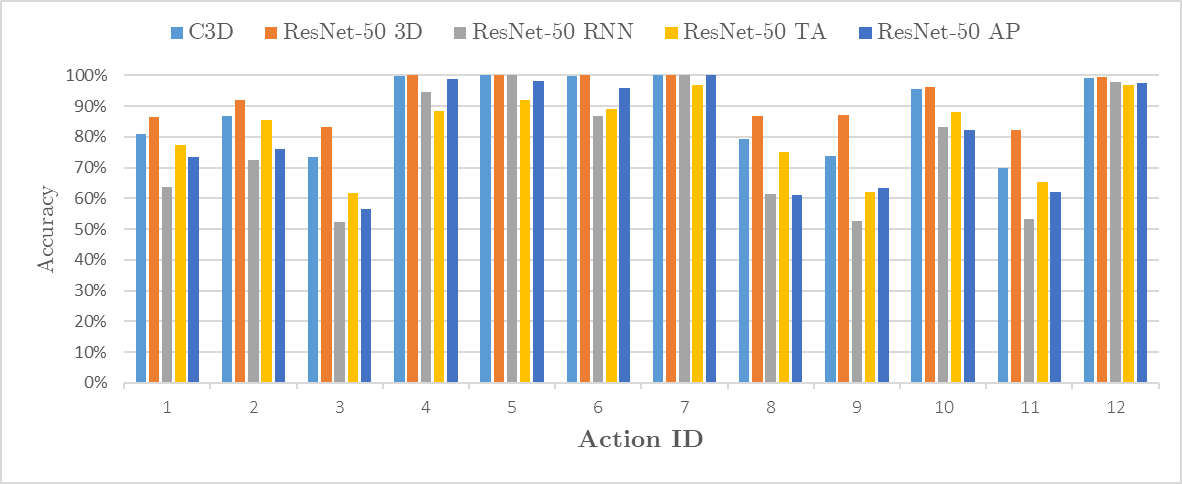
\includegraphics[width=0.8\linewidth]{figs/pc-MvDA_confusion_ixmas.png}
        \caption{Comparison of accuracy on each action class using different deep features combined with pc-MvDA on IXMAS dataset.}
        %\vspace{-0.3cm}
        \label{fig:pc-MvDA_confusion_ixmas}
    \end{figure}

    Table \ref{tab:sota_ixmas} compares the best combination of ResNet-50 3D and pc-MvDA with state-of-the-art frameworks. The comparison is for reference only because in other works, low-level hand-crafted video representation is used as private features and train-test strategy is leave-one-class out, which is not applicable to supervised deep feature extractors in this work. However, the results are still commensurable. % in circumstances where supervised approaches are adopted.
    % TODO - High priority

    \begin{table}[htbp]
    \centering
    \caption{Comparison of proposed methods with SOTA methods on IXMAS dataset according to the second evaluation protocol.}
    \resizebox{0.7\textwidth}{!}{
    \begin{tabular}{|c|c|c|}
    \hline
    Methods                                                              & Cross-view & Multi-view \\ \hline
    Liu et al. \cite{liu2011cross}                                   & 76.32      & N/A       \\ \hline
    Zheng et al. \cite{zheng2012cross}                               & 95.1       & 99.32     \\ \hline
    Zheng et al. \cite{zheng2016cross}                               & 97.8       & 99.4      \\ \hline
    Kong et al. \cite{kong2017deeply}                                & 99.92      & 100       \\ \hline
    Ulhaq et al. \cite{ulhaq2017space}                               & 66.82      & 92.47     \\ \hline
    Zhang et al. \cite{zhang2018cross}                               & 84.1       & N/A        \\ \hline
    Liu et al. \cite{liu2018learning}                                & N/A        & 90.3     \\ \hline
    Liu et al. \cite{liu2018hierarchically}                          & 99.95      & 99.67     \\ \hline
    Proposed method (ResNet-50 3D + pc-MvDA)                     & 99.67      & 99.65       \\ \hline
    \end{tabular}}
    \label{tab:sota_ixmas}
    \end{table}

    %!TEX root = ../../../main.tex

\subsection{Experimental results on MuHAVi dataset}
    \paragraph{1) Cross-view validation:} Table.\ref{tab:muhavi_cross} illustrates cross-view recognition results. The proposed pc-MvDA consistently produces a better average accuracy of around 96.19\% for protocol 1, approximately 4.55\% and 1.51\% higher than that of MvDA (91.64\%) and MvDA-vc (94.67\%) respectively.

    \begin{table}[htbp]
    \centering
    \caption{Cross-view recognition comparison on MuHAVi dataset.}
    \resizebox{0.8\textwidth}{!}{
    \begin{tabular}{|c|c|c|c|c|c|c|}
        \hline
        \multirow{2}{*}{Deep features}          & \multicolumn{3}{c|}{Protocol 1}   & \multicolumn{3}{c|}{Protocol 2}           \\ \cline{2-7} 
                                                & MvDA  & MvDA-vc & pc-MvDA         & MvDA  & MvDA-vc        & pc-MvDA          \\ \hline
        \multicolumn{1}{|c|}{C3D}               & 92.85 & 95.15   & \textbf{97.65}  & 98.95 & 99.76          & \textbf{100}     \\ \hline
        \multicolumn{1}{|c|}{ResNet-50 3D}      & 97.94 & 99.15   & \textbf{99.18}  & 96.77 & \textbf{99.94} & \textbf{99.94}   \\ \hline
        \multicolumn{1}{|c|}{ResNet-50 RNN}     & 95.54 & 95.14   & \textbf{96.18}  & 98.70 & 99.05          & \textbf{99.99}   \\ \hline
        \multicolumn{1}{|c|}{ResNet-50 TA}      & 85.80 & 88.95   & \textbf{91.12}  & 96.57 & 97.03          & \textbf{99.88}   \\ \hline
        \multicolumn{1}{|c|}{ResNet-50 AP}      & 86.09 & 94.98   & \textbf{96.82}  & 89.04 & 98.62          & \textbf{99.93}   \\ \hline
    \end{tabular}}
    \label{tab:muhavi_cross}
    \end{table}

    %Results in Table.\ref{tab:cross_feature_muhavi} show that our combination with ResNet-50 3D has the highest accuracies in almost every circumstances, even though both features coupled with our proposed pc-MvDA give satisfactory performance with all scores exceeding 91\%.

    \begin{table}[htbp]
    \centering
    \caption{Cross-view recognition results of different features on MuHAVi dataset with pc-MvDA method. The result in the bracket are accuracies of using features C3D, ResNet-50 3D, ResNet-50 RNN, ResNet-50 TA, ResNet-50 AP respectively. Each row corresponds to training view (from view C1 to view C7). Each column corresponds to testing view (from view C1 to view C7).}
    \resizebox{\textwidth}{!}{\begin{tabular}{|c|c|c|c|c|c|c|c|}
        \hline
        \backslashbox{Training}{Testing} & C1 & C2 & C3 & C4 & C5 & C6 & C7 \\ \hline
        C1 & N/A & \begin{tabular}{@{}c@{}} (96.1, \textbf{100}, 96.8, \\ 88.5, 98.5) \end{tabular} & \begin{tabular}{@{}c@{}} (98.6, \textbf{99.6}, 96.6, \\ 88.9, 96.3) \end{tabular} & \begin{tabular}{@{}c@{}} (98.6, \textbf{99.6}, 98.0, \\ 93.1, 98.2) \end{tabular} & \begin{tabular}{@{}c@{}} (97.7, \textbf{99.6}, 95.4, \\ 91.3, 96.1) \end{tabular} & \begin{tabular}{@{}c@{}} (97.7, \textbf{98.4}, 92.3, \\ 93.1, 96.3) \end{tabular} & \begin{tabular}{@{}c@{}} (98.2, \textbf{98.5}, 97.2, \\ 89.8, 97.1) \end{tabular} \\ \hline
        C2 & \begin{tabular}{@{}c@{}} (95.6, \textbf{99.0}, 95.2, \\ 91.3, 95.5) \end{tabular} & N/A & \begin{tabular}{@{}c@{}} (98.9, \textbf{99.6}, 96.9, \\ 90.3, 96.1) \end{tabular} & \begin{tabular}{@{}c@{}} (98.4, \textbf{99.6}, 97.6, \\ 92.6, 98.2) \end{tabular} & \begin{tabular}{@{}c@{}} (97.7, \textbf{99.6}, 95.4, \\ 90.9, 96.1) \end{tabular} & \begin{tabular}{@{}c@{}} (97.8, \textbf{98.4}, 92.7, \\ 93.6, 96.5) \end{tabular} & \begin{tabular}{@{}c@{}} (98.6, \textbf{99.0}, 97.4, \\ 90.6, 96.9) \end{tabular} \\ \hline
        C3 & \begin{tabular}{@{}c@{}} (96.1, \textbf{99.0}, 95.6, \\ 90.3, 95.1) \end{tabular} & \begin{tabular}{@{}c@{}} (97.0, \textbf{100}, 96.7, \\ 88.4, 97.8) \end{tabular} & N/A & \begin{tabular}{@{}c@{}} (98.1, \textbf{99.2}, 98.2, \\ 92.8, 98.2) \end{tabular} & \begin{tabular}{@{}c@{}} (97.9, \textbf{99.6}, 95.4, \\ 90.2, 95.6) \end{tabular} & \begin{tabular}{@{}c@{}} (97.9, \textbf{98.2}, 93.0, \\ 94.2, 96.5) \end{tabular} & \begin{tabular}{@{}c@{}} (97.8, \textbf{98.7}, 97.4, \\ 89.4, 97.6) \end{tabular} \\ \hline
        C4 & \begin{tabular}{@{}c@{}} (96.4, \textbf{98.8}, 95.4, \\ 89.6, 95.3) \end{tabular} & \begin{tabular}{@{}c@{}} (96.3, \textbf{100}, 96.6, \\ 91.0, 98.5) \end{tabular} & \begin{tabular}{@{}c@{}} (98.6, \textbf{99.6}, 97.3, \\ 89.5, 96.1) \end{tabular} & N/A & \begin{tabular}{@{}c@{}} (97.7, \textbf{99.4}, 95.6, \\ 91.3, 96.1) \end{tabular} & \begin{tabular}{@{}c@{}} (\textbf{98.4}, 98.0, 93.2, \\ 93.8, 95.6) \end{tabular} & \begin{tabular}{@{}c@{}} (97.7, \textbf{98.7}, 97.4, \\ 91.3, 96.7) \end{tabular} \\ \hline
        C5 & \begin{tabular}{@{}c@{}} (95.9, \textbf{99.0}, 95.6, \\ 91.3, 95.5) \end{tabular} & \begin{tabular}{@{}c@{}} (96.6, \textbf{100}, 97.1, \\ 89.9, 98.3) \end{tabular} & \begin{tabular}{@{}c@{}} (98.8, \textbf{99.4}, 96.8, \\ 90.7, 96.1) \end{tabular} & \begin{tabular}{@{}c@{}} (98.4, \textbf{99.6}, 98.0, \\ 92.1, 97.6) \end{tabular} & N/A & \begin{tabular}{@{}c@{}} (97.9, \textbf{98.2}, 93.4, \\ 94.4, 96.8) \end{tabular} & \begin{tabular}{@{}c@{}} (98.0, \textbf{98.7}, 96.9, \\ 89.0, 97.8) \end{tabular} \\ \hline
        C6 & \begin{tabular}{@{}c@{}} (95.8, \textbf{99.0}, 95.8, \\ 90.3, 95.0) \end{tabular} & \begin{tabular}{@{}c@{}} (97.0, \textbf{100}, 97.6, \\ 89.7, 98.5) \end{tabular} & \begin{tabular}{@{}c@{}} (98.8, \textbf{99.6}, 96.9, \\ 88.7, 96.1) \end{tabular} & \begin{tabular}{@{}c@{}} (98.4, \textbf{99.4}, 98.0, \\ 92.8, 98.2) \end{tabular} & \begin{tabular}{@{}c@{}} (97.5, \textbf{99.6}, 95.9, \\ 91.2, 95.5) \end{tabular} & N/A & \begin{tabular}{@{}c@{}} (98.2, \textbf{99.0}, 97.2, \\ 90.7, 97.4) \end{tabular} \\ \hline
        C7 & \begin{tabular}{@{}c@{}} (96.2, \textbf{98.8}, 95.7, \\ 91.5, 96.2) \end{tabular} & \begin{tabular}{@{}c@{}} (96.4, \textbf{100}, 97.5, \\ 90.3, 98.5) \end{tabular} & \begin{tabular}{@{}c@{}} (98.4, \textbf{99.0}, 97.3, \\ 90.0, 96.7) \end{tabular} & \begin{tabular}{@{}c@{}} (\textbf{98.8}, 98.8, 98.2, \\ 92.8, 98.0) \end{tabular} & \begin{tabular}{@{}c@{}} (97.5, \textbf{99.8}, 95.9, \\ 91.5, 95.9) \end{tabular} & \begin{tabular}{@{}c@{}} (\textbf{98.9}, 98.2, 92.8, \\ 93.9, 97.1) \end{tabular} & N/A \\ \hline
    \end{tabular}}
    \label{tab:cross_feature_muhavi}
    \end{table}

    \paragraph{2) Multi-view validation}: Table.\ref{tab:muhavi_multi} shows multi-view recognition results. The first protocol shows very close capability of MvDA-vc and pc-MvDA at 95.54\% and 95.83\% whereas MvDA is about 3\% behind at 92.7\%. For the second protocol, our variant exceeds MvDA by 2.21\% and MvDA-vc by 1.49\%. The near perfect results of the second protocol give us the same indication that it is not an inequitable method of comparison of MvA algorithms. 

    \begin{table}[htbp]
    \centering
    \caption{Multi-view recognition comparison on MuHAVi dataset.}
    \resizebox{0.8\textwidth}{!}{
    \begin{tabular}{|c|c|c|c|c|c|c|}
        \hline
        \multirow{2}{*}{Deep features}          & \multicolumn{3}{c|}{Protocol 1}                   & \multicolumn{3}{c|}{Protocol2}            \\ \cline{2-7} 
                                                & MvDA           & MvDA-vc        & pc-MvDA         & MvDA           & MvDA-vc & pc-MvDA        \\ \hline
        \multicolumn{1}{|c|}{C3D}               & 81.80          & 96.05          & \textbf{97.37}  & 88.39          & 99.61   & \textbf{100}   \\ \hline
        \multicolumn{1}{|c|}{ResNet-50 3D}      & 99.07          & 99.12          & \textbf{99.15}  & \textbf{99.98} & 99.96   & 99.89          \\ \hline
        \multicolumn{1}{|c|}{ResNet-50 RNN}     & \textbf{96.18} & 95.55          & 95.97           & \textbf{100}   & 99.00   & 99.98          \\ \hline
        \multicolumn{1}{|c|}{ResNet-50 TA}      & \textbf{90.45} & 89.73          & 90.22           & \textbf{99.92} & 98.17   & 99.72          \\ \hline
        \multicolumn{1}{|c|}{ResNet-50 AP}      & 96.01          & \textbf{96.75} & 96.42           & \textbf{100}   & 95.13   & 99.68          \\ \hline
    \end{tabular}}
    \label{tab:muhavi_multi}
    \end{table}

    Figure \ref{fig:pc-MvDA_confusion_muhavi} compares the performance of feature extractors regarding each action class in multi-view evaluation scheme combined with protocol 1. For this dataset, ResNet-50 3D persistently yields out-standing performance while ResNet-50 TA has the worst recognition rates in all action classes.

    \begin{figure}[htbp]
        \centering
        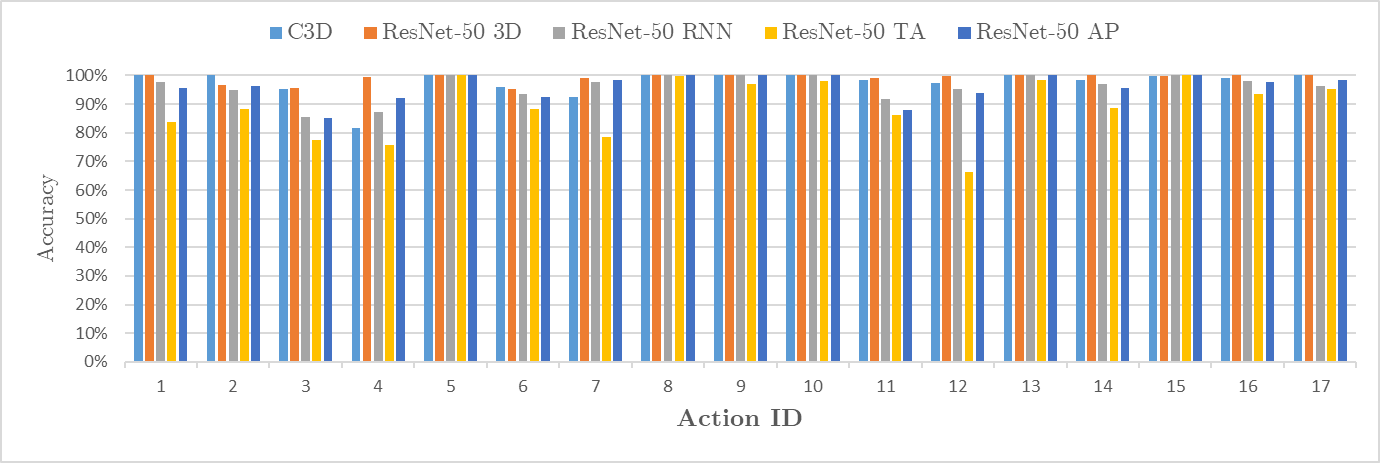
\includegraphics[width=1.0\linewidth]{figs/pc-MvDA_confusion_muhavi.png}
        \caption{Comparison of accuracy on each action class using different deep features combined with pc-MvDA.}
        %\vspace{-0.3cm}
        \label{fig:pc-MvDA_confusion_muhavi}
    \end{figure}

    Table \ref{tab:sota_muhavi} compares the best investigated combination of ResNet-50 3D and pc-MvDA with state-of-the-art frameworks. The comparison is for reference only because of aforementioned difference in setup of number of views and cross validation scheme.

    \begin{table}[htbp]
    \centering
    \caption{Comparison of the proposed methods with SOTA methods on MuHAVi dataset according to the second evaluation protocol.}
    \resizebox{0.7\textwidth}{!}{
    \begin{tabular}{|c|c|c|}
    \hline
    Methods                                                   & Cross-view & Multi-view \\ \hline
    Wu et al. \cite{wu2012view}                               & N/A       & 94.5     \\ \hline
    Zheng et al. \cite{zheng2016cross}                        & 94.88     & 99.8     \\ \hline
    Liu et al. \cite{liu2018learning}                         & N/A       & 91.2     \\ \hline
    Liu et al. \cite{liu2018hierarchically}                   & 99.91     & 99.8     \\ \hline
    Proposed method (ResNet-50 3D + pc-MvDA) \protect\footnotemark              & 99.90     & 99.88    \\ \hline
    \end{tabular}}
    \label{tab:sota_muhavi}
    \end{table}
    \footnotetext{Results when choosing only 4 views Camera 1, Camera 3, Camera 4 and Camera 6 following the other works.}

    %!TEX root = ../../../main.tex

\subsection{Experimental results on MICAGes dataset}

    \paragraph{1) Cross-view validation:} It can be seen in Table.\ref{tab:mica_cross} that pc-MvDA outperforms in almost every cases. With the first protocol, the norm accuracy of pc-MvDA of 74.52\% surpasses that of MvDA-vc (72.12\%) by 2.4\% and that of MvDA (64.94\%) by a large margin of 9.58\%. Especially in case of C3D features, the proposed algorithm achieved 90.2\% recognition rate whereas MvDA returns only 67.13\%.

    \begin{table}[htbp]
    \centering
    \caption{Cross-view recognition comparison on MICAGes dataset.}
    \resizebox{0.8\textwidth}{!}{
    \begin{tabular}{|c|c|c|c|c|c|c|}
        \hline
        \multirow{2}{*}{Deep features}          & \multicolumn{3}{c|}{Protocol 1}          & \multicolumn{3}{c|}{Protocol 2}            \\ \cline{2-7} 
                                                & MvDA  & MvDA-vc        & pc-MvDA         & MvDA  & MvDA-vc        & pc-MvDA           \\ \hline
        \multicolumn{1}{|c|}{C3D}               & 67.13 & 85.98          & \textbf{90.20}  & 93.74 & 99.80          & \textbf{100}      \\ \hline
        \multicolumn{1}{|c|}{ResNet-50 3D}      & 94.91 & 95.25          & \textbf{95.62}  & 97.43 & \textbf{99.97} & 99.79             \\ \hline
        \multicolumn{1}{|c|}{ResNet-50 RNN}     & 58.01 & 61.64          & \textbf{64.13}  & 100   & 100            & 100               \\ \hline
        \multicolumn{1}{|c|}{ResNet-50 TA}      & 53.58 & \textbf{59.55} & 58.62           & 96.70 & 99.48          & \textbf{99.83}    \\ \hline
        \multicolumn{1}{|c|}{ResNet-50 AP}      & 51.07 & 58.19          & \textbf{64.04}  & 99.73 & \textbf{99.99} & 99.89             \\ \hline
    \end{tabular}}
    \label{tab:mica_cross}
    \end{table}

    %Table.\ref{tab:cross_feature_mica} compares all types of deep features regarding accuracy of the proposed algorithm. 
    The top ranking of features applies identically and radically proves the superiority of 3D convolution based clip-level feature extraction in video recognition: ResNet-50 3D at 95.62\% and C3D at 90.2\%. The rest are ResNet-50 RNN (64.13\%), ResNet-50 AP (64.04\%) and ResNet-50 TA (58.62\%). For the second protocol, MvDA-vc (99.85\%) and pc-MvDA (99.9\%) are nearly even in performance while MvDA achieved 97.52\%.

    \begin{table}[htbp]
    \centering
    \caption{Cross-view recognition results of different features on MICAGes dataset with pc-MvDA method. The result in the bracket are accuracies of using features C3D, ResNet-50 3D, ResNet-50 RNN, ResNet-50 TA, RestNet-50 AP respectively. Each row corresponds to training view (from view K1 to view K5). Each column corresponds to testing view (from view K1 to view K5).}
    \resizebox{\textwidth}{!}{\begin{tabular}{|c|c|c|c|c|c|}
        \hline
        \backslashbox{Training}{Testing} & K1 & K2 & K3 & K4 & K5 \\ \hline
        K1 & N/A & \begin{tabular}{@{}c@{}} (92.9, \textbf{95.5}, 69.4, \\ 63.9, 65.1) \end{tabular} & \begin{tabular}{@{}c@{}} (93.7, \textbf{98.0}, 79.1, \\ 75.8, 74.7) \end{tabular} & \begin{tabular}{@{}c@{}} (90.5, \textbf{97.6}, 64.5, \\ 68.8, 70.8) \end{tabular} & \begin{tabular}{@{}c@{}} (89.2, \textbf{92.6}, 56.0, \\ 43.7, 58.2) \end{tabular} \\ \hline       
        K2 & \begin{tabular}{@{}c@{}} (84.7, \textbf{94.6}, 51.3, \\ 41.4, 53.7) \end{tabular} & N/A & \begin{tabular}{@{}c@{}} (94.6, \textbf{97.6}, 78.9, \\ 75.4, 77.5) \end{tabular} & \begin{tabular}{@{}c@{}} (91.3, \textbf{97.6}, 64.4, \\ 68.5, 68.0) \end{tabular} & \begin{tabular}{@{}c@{}} (87.4, \textbf{92.7}, 56.1, \\ 42.0, 55.6) \end{tabular} \\ \hline       
        K3 & \begin{tabular}{@{}c@{}} (87.5, \textbf{94.9}, 51.9, \\ 43.6, 52.7) \end{tabular} & \begin{tabular}{@{}c@{}} (93.0, \textbf{95.5}, 70.1, \\ 64.7, 63.4) \end{tabular} & N/A & \begin{tabular}{@{}c@{}} (90.0, \textbf{97.6}, 63.2, \\ 62.6, 67.5) \end{tabular} & \begin{tabular}{@{}c@{}} (88.9, \textbf{92.2}, 57.2, \\ 41.8, 56.6) \end{tabular} \\ \hline       
        K4 & \begin{tabular}{@{}c@{}} (86.7, \textbf{94.7}, 50.8, \\ 48.9, 54.9) \end{tabular} & \begin{tabular}{@{}c@{}} (90.2, \textbf{95.5}, 71.5, \\ 68.2, 61.8) \end{tabular} & \begin{tabular}{@{}c@{}} (92.5, \textbf{98.0}, 81.0, \\ 76.0, 74.4) \end{tabular} & N/A & \begin{tabular}{@{}c@{}} (89.7, \textbf{92.3}, 54.3, \\ 44.9, 56.6) \end{tabular} \\ \hline       
        K5 & \begin{tabular}{@{}c@{}} (84.9, \textbf{94.9}, 48.4, \\ 41.5, 57.9) \end{tabular} & \begin{tabular}{@{}c@{}} (90.4, \textbf{95.5}, 72.6, \\ 64.1, 65.7) \end{tabular} & \begin{tabular}{@{}c@{}} (94.0, \textbf{97.8}, 79.1, \\ 72.5, 76.3) \end{tabular} & \begin{tabular}{@{}c@{}} (91.9, \textbf{97.3}, 62.7, \\ 64.1, 69.0) \end{tabular} & N/A \\ \hline
    \end{tabular}}
    \label{tab:cross_feature_mica}
    \end{table}

    \paragraph{2) Multi-view validation}: The multi-view recognition results in Table.\ref{tab:mica_multi} shows an almost alike trend for both protocols. In general, pc-MvDA is 8.95\% and 0.72\% higher in accuracy for protocol 1, and 2.75\% and 0.04\% for protocol 2, in comparison with MvDA and MvDA-pc respectively.

    % TODO
    In virtually every experiments of MICAGes and two earlier benchmark datasets, the proposed extension is superior. The average accuracies of pc-MvDA is, in comparison on protocol 1 (and protocol 2 resp.), 5.29\% (1.21\% resp.) higher than MvDA, 1.21\% (0.62\% resp.) better than MvDA-vc. Despite not being as intuitive and straightly intelligible as pairwise-covariance, the multi-view resemblance added in MvDA-vc achieved nearly the performance of pc-MvDA. However, this view-consistency can be easily splitted into pairwise terms and intergrated into the objective of pc-MvDA in future works for further analysis.

    \begin{table}[htbp]
    \centering
    \caption{Multi-view recognition comparison on MICAGes dataset.}
    \resizebox{0.8\textwidth}{!}{
    \begin{tabular}{|c|c|c|c|c|c|c|}
        \hline
        \multirow{2}{*}{Deep features}          & \multicolumn{3}{c|}{Protocol 1}          & \multicolumn{3}{c|}{Protocol2}                     \\ \cline{2-7} 
                                                & MvDA  & MvDA-vc        & pc-MvDA         & MvDA           & MvDA-vc       & pc-MvDA           \\ \hline
        \multicolumn{1}{|c|}{C3D}               & 68.31 & 87.70          & \textbf{89.99}  & 88.79          & 99.54         & \textbf{100}      \\ \hline
        \multicolumn{1}{|c|}{ResNet-50 3D}      & 95.32 & 95.26          & \textbf{95.54}  & \textbf{100}   & 99.96         & 99.80             \\ \hline
        \multicolumn{1}{|c|}{ResNet-50 RNN}     & 57.50 & 63.05          & \textbf{63.83}  & 99.90          & \textbf{100}  & 99.97             \\ \hline
        \multicolumn{1}{|c|}{ResNet-50 TA}      & 54.43 & \textbf{61.46} & 58.25           & 96.72          & 99.49         & \textbf{99.69}    \\ \hline
        \multicolumn{1}{|c|}{ResNet-50 AP}      & 50.93 & 60.20          & \textbf{63.66}  & \textbf{99.99} & 99.93         & 99.67             \\ \hline
    \end{tabular}}
    \label{tab:mica_multi}
    \end{table}

    In addition to the same propensity shown, MICAGes also reveals the robustness of 3D convolution to generate fine clustered private feature space because this dataset contains exclusively hand gestures, which take part in a relatively small region of the captured videos. ResNet-50 3D and C3D are predominant for discriminant common space construction and classification and distances other features (Figure \ref{fig:pc-MvDA_confusion_mica}).

    \begin{figure}[htbp]
        \centering
        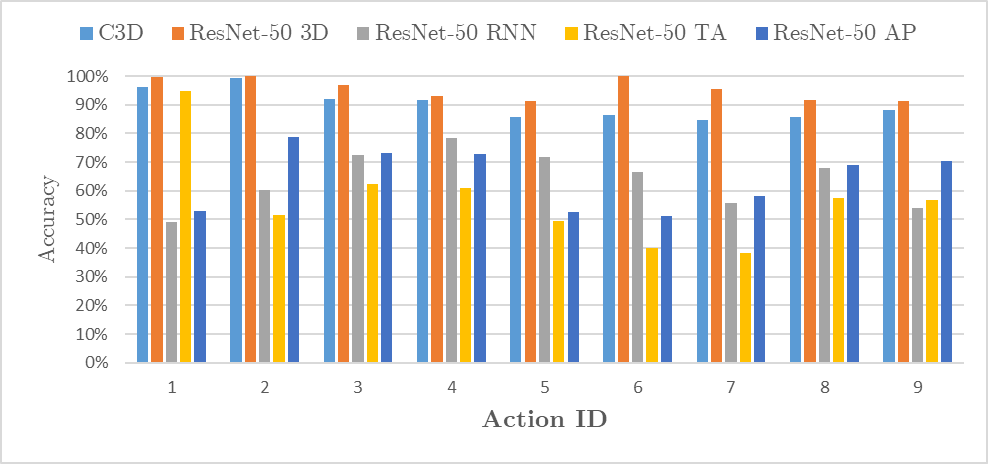
\includegraphics[width=0.8\linewidth]{figs/pc-MvDA_confusion_mica.png}
        \caption{Comparison of accuracy on each action class using different deep features combined with pc-MvDA on MICAGes dataset.}
        %\vspace{-0.3cm}
        \label{fig:pc-MvDA_confusion_mica}
    \end{figure}

    To better study the behavior of investigated multi-view analysis algorithms, t-SNE embedding of original private spaces, MvDA and pc-MvDA common space generated by protocol 1 are plotted in Figure \ref{fig:mica-tsne}. In these scatter plots, colors denote action classes, shapes as different views and train/test data are distinguished by border type. They explicitly denotes the surpassing capability of the proposed algorithm in finding a common space with prominent extra-class discrepancy. The data samples involved in training process are generally clustered in compact and separated blobs while testing data samples dissolve nearby. The better convergence of pc-MvDA compared to the baseline is usually only visible for harder features, whereas with the inputs of ResNet-50 3D features, which are already highly discriminated in private spaces, the improvement of pc-MvDA is negligible. Note that these illustrations of t-SNE embedding do not strictly depict an identical distribution of data.

    \begin{figure}[htbp]
        \centering
        \includegraphics[width=1\linewidth, height=0.6\pdfpageheight, keepaspectratio=false]{figs/mica-tsne.png}
        \caption{First column: private feature spaces stacked and embedded together in a same coordinate system; Second column: MvDA common space; Third column: pc-MvDA common space.}
        %\vspace{-0.3cm}
        \label{fig:mica-tsne}
    \end{figure}


    %!TEX root = ../../../main.tex

\section{Experimental Results and Discussions} \label{sec:results}
    %!TEX root = ../../../main.tex

\subsection{Experimental results on IXMAS dataset}
    \paragraph{1) Cross-view validation:} In this experiment, we train on data from one view (training view) and testing on data from another view (testing view) then compute the accuracies for two evaluation protocols. Table \ref{tab:cross_p1_ixmas} shows comparative results of using different deep features (C3D, ResNet-50 3D, ResNet-50 RNN, ResNet-50 TA, ResNet-50 AP) and multi-view discriminant analysis techniques (MvDA, MvDA-vc and our proposed pc-MvDA). 

    With the first evaluation protocol, the proposed pc-MvDA, when combined with deep features, gives mostly best accuracy for both evaluation protocols. With C3D features, accuracy by pc-MvDA (88.43\%) is 6.6\% higher than MvDA (81.84\%). pc-MvDA is even better than MvDA-vc (2.87\%). pc-MvDA achieved higher accuracy (about 6\% higher) than MvDA and MvDA-vc with ResNet-50 TA and ResNet-50 AP features. In average, pc-MvDA is 3.09\% higher than MvDA and 1.4\% higher than MvDA-vc.
    
    \begin{table}[htbp]
    \centering
    \caption{Cross-view recognition comparison on IXMAS dataset.}
    \resizebox{0.8\textwidth}{!}{
    \begin{tabular}{|l|c|c|c|c|c|c|}
        \hline
        \multirow{2}{*}{Deep features}          & \multicolumn{3}{c|}{Protocol 1}   & \multicolumn{3}{c|}{Protocol 2}           \\ \cline{2-7} 
                                                & MvDA  & MvDA-vc & pc-MvDA         & MvDA  & MvDA-vc        & pc-MvDA          \\ \hline
        \multicolumn{1}{|c|}{C3D}               & 81.84 & 85.56   & \textbf{88.43}  & 96.54 & 99.29          & \textbf{99.98}   \\ \hline
        \multicolumn{1}{|c|}{ResNet-50 3D}      & 91.25 & 92.19   & \textbf{92.89}  & 97.30 & \textbf{99.73} & 99.65            \\ \hline
        \multicolumn{1}{|c|}{ResNet-50 RNN}     & 75.51 & 76.12   & \textbf{76.54}  & 99.99 & 99.71          & \textbf{100}     \\ \hline
        \multicolumn{1}{|c|}{ResNet-50 TA}      & 79.44 & 80.58   & \textbf{82.05}  & 99.33 & 99.34          & \textbf{99.84}   \\ \hline
        \multicolumn{1}{|c|}{ResNet-50 AP}      & 77.00 & 79.04   & \textbf{80.58}  & 99.68 & 99.81          & \textbf{99.92}   \\ \hline
    \end{tabular}}
    \label{tab:cross_p1_ixmas}
    \end{table}

    For the second evaluation protocol, pc-MvDA almost always keeps better performance compared to MvDA and MvDA-vc. The recognition accuracy scores obtained by both pc-MvDA and MvDA-vc are nearly 100\% for every kind of deep features. With C3D features and ResNet-50 3D features, pc-MvDA is 99.98\% and 99.65\%, which is 3.44\% and 2.35\% higher than the orginal MvDA (96.54\% and 97.3\%) respectively. In average, pc-MvDA is 1.31\% better than MvDA and 0.3\% better than MvDA-vc. 

    In terms of deep features, with the first evaluation protocol, ResNet-50 3D gives the best accuracy (92.89\%) following by C3D (88.43\%), ResNet-50 TA (82.05\%), ResNet-50 AP (80.58\%). The lowest accuracy obtained by ResNet-50 RNN is only 76.54\%. It shows that ResNet-50 3D produces the most discriminative feature space. %Table \ref{tab:cross_feature_ixmas} shows comparative results when using pc-MvDA method with different deep features regarding pairwise views. 

    \begin{table}[htbp]
    \centering
    \caption{Cross-view recognition results of different features on IXMAS dataset with pc-MvDA method. The result in the bracket are accuracies of using features C3D, ResNet-50 3D, ResNet-50 RNN, ResNet-50 TA, Restnet-50 AP respectively. Each row corresponds to training view (from view C0 to view C3). Each column corresponds to testing view (from view C0 to view C3).}
    \resizebox{\textwidth}{!}{\begin{tabular}{|c|c|c|c|c|}
        \hline
        \backslashbox{Training}{Testing} & C0 & C1 & C2 & C3 \\ \hline
        C0 & N/A & (90.7, \textbf{91.9}, 81.6, 84.6, 83.6) & (86.9, \textbf{93.9}, 78.0, 79.6, 78.1) & (89.9, \textbf{93.4}, 76.3, 82.8, 82.1) \\ \hline
        C1 & (86.6, \textbf{91.9}, 71.5, 81.1, 77.5) & N/A & (85.9, \textbf{94.2}, 78.6, 79.3, 80.3) & (88.9, \textbf{93.7}, 74.8, 82.3, 81.3) \\ \hline
        C2 & (87.6, \textbf{92.4}, 72.8, 81.8, 78.5) & (90.7, \textbf{91.7}, 80.6, 83.6, 82.6) & N/A & (89.4, \textbf{93.7}, 75.5, 82.3, 80.6) \\ \hline
        C3 & (87.6, \textbf{92.9}, 70.2, 82.1, 78.8) & (90.7, \textbf{91.2}, 81.6, 84.1, 82.8) & (86.4, \textbf{93.7}, 77.3, 80.6, 80.8) & N/A \\ \hline
    \end{tabular}}
    \label{tab:cross_feature_ixmas}
    \end{table}

    \paragraph{2) Multi-view validation} Table \ref{tab:ixmas_multi} shows multi-view recognition results. The conclusion is consistent with the case of cross-view evaluation: ResNet-50 3D is the best feature extractor. When it is combined with pc-MvDA, the framework gives the highest accuracy for the first protocol (92.82\%), following by C3D (88.19\%), ResNet-50 TA (81.49\%), ResNet-50 AP(80.43\%), and ResNet-50 RNN (76.47\%). Both MvA algorithms give similar accuracies for the second evaluation protocols (nearly 100\%). Again, pc-MvDA enhances the performance of MvDA by 2.43\% for the first protocol and 0.83\% for the second protocol. It only gives slightly better result than MvDA-vc (0.83\% for the first protocol and 0.74\% for the second protocol). 

    \begin{table}[htbp]
    \centering
    \caption{Multi-view recognition comparison on IXMAS dataset.}
    \resizebox{0.7\textwidth}{!}{\begin{tabular}{|c|c|c|c|c|c|c|}
        \hline
        \multirow{2}{*}{Deep features}          & \multicolumn{3}{c|}{Protocol 1}   & \multicolumn{3}{c|}{Protocol2}                    \\ \cline{2-7} 
                                                & MvDA  & MvDA-vc & pc-MvDA         & MvDA           & MvDA-vc        & pc-MvDA         \\ \hline
        \multicolumn{1}{|c|}{C3D}               & 86.93 & 87.04   & \textbf{88.19}  & \textbf{99.99} & 99.44          & \textbf{99.98}  \\ \hline
        \multicolumn{1}{|c|}{ResNet-50 3D}      & 91.84 & 92.33   & \textbf{92.82}  & \textbf{100}   & 99.80          & 99,67           \\ \hline
        \multicolumn{1}{|c|}{ResNet-50 RNN}     & 72.44 & 75.95   & \textbf{76.47}  & 99.34          & \textbf{99.97} & \textbf{99.96}  \\ \hline
        \multicolumn{1}{|c|}{ResNet-50 TA}      & 76.74 & 81.01   & \textbf{81.49}  & 95.80          & 98.25          & \textbf{99.79}  \\ \hline
        \multicolumn{1}{|c|}{ResNet-50 AP}      & 79.28 & 78.93   & \textbf{80.43}  & \textbf{100}   & 98.11          & 99.85           \\ \hline
    \end{tabular}}
    \label{tab:ixmas_multi}
    \end{table}

    Figure \ref{fig:pc-MvDA_confusion_ixmas} compares the performance of feature extractors regarding each action class in multi-view evaluation scheme combined with the first evaluation protocol. There are clear margins between the performance of ResNet-50 3D and followed by C3D with other types of deep features, especially in harder actions (the first class to the third class and the eighth class to the eleventh class). These actions (check watch, cross arm, scratch head, wave, punch, kick, point) involve the most part static pose of the body and only movement of limbs, whereas other actions 4 - sit down, 5 - get up, 6 - turn around, 7 - walk and 12 - pickup include movement of the whole body and are easier to be recognized. This suggests that 3D convolution can better deal with small difference of movement in action images, which in turn generates a much more classification-ready feature space for latter stage of recognition.

    \begin{figure}[htbp]
        \centering
        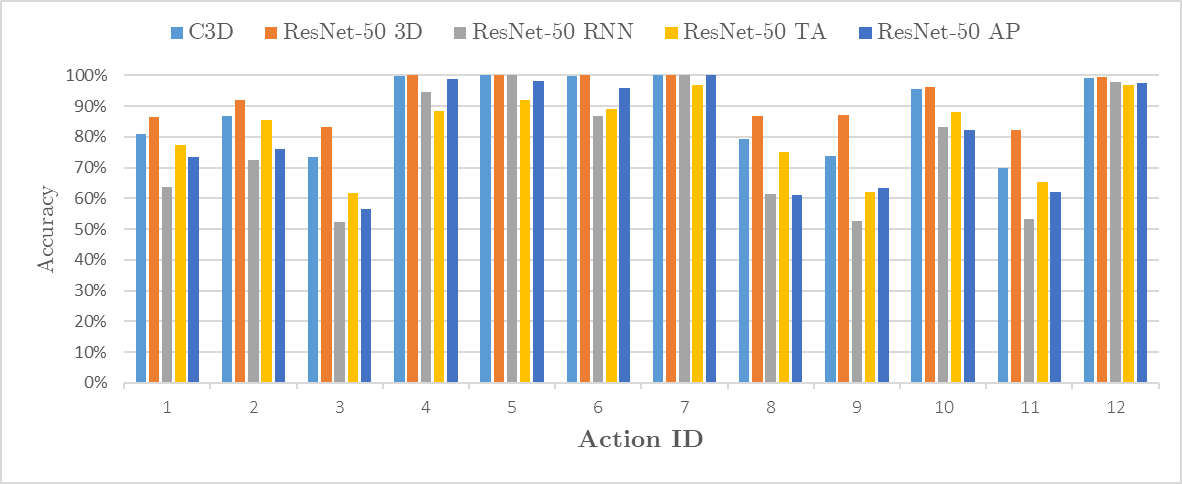
\includegraphics[width=0.8\linewidth]{figs/pc-MvDA_confusion_ixmas.png}
        \caption{Comparison of accuracy on each action class using different deep features combined with pc-MvDA on IXMAS dataset.}
        %\vspace{-0.3cm}
        \label{fig:pc-MvDA_confusion_ixmas}
    \end{figure}

    Table \ref{tab:sota_ixmas} compares the best combination of ResNet-50 3D and pc-MvDA with state-of-the-art frameworks. The comparison is for reference only because in other works, low-level hand-crafted video representation is used as private features and train-test strategy is leave-one-class out, which is not applicable to supervised deep feature extractors in this work. However, the results are still commensurable. % in circumstances where supervised approaches are adopted.
    % TODO - High priority

    \begin{table}[htbp]
    \centering
    \caption{Comparison of proposed methods with SOTA methods on IXMAS dataset according to the second evaluation protocol.}
    \resizebox{0.7\textwidth}{!}{
    \begin{tabular}{|c|c|c|}
    \hline
    Methods                                                              & Cross-view & Multi-view \\ \hline
    Liu et al. \cite{liu2011cross}                                   & 76.32      & N/A       \\ \hline
    Zheng et al. \cite{zheng2012cross}                               & 95.1       & 99.32     \\ \hline
    Zheng et al. \cite{zheng2016cross}                               & 97.8       & 99.4      \\ \hline
    Kong et al. \cite{kong2017deeply}                                & 99.92      & 100       \\ \hline
    Ulhaq et al. \cite{ulhaq2017space}                               & 66.82      & 92.47     \\ \hline
    Zhang et al. \cite{zhang2018cross}                               & 84.1       & N/A        \\ \hline
    Liu et al. \cite{liu2018learning}                                & N/A        & 90.3     \\ \hline
    Liu et al. \cite{liu2018hierarchically}                          & 99.95      & 99.67     \\ \hline
    Proposed method (ResNet-50 3D + pc-MvDA)                     & 99.67      & 99.65       \\ \hline
    \end{tabular}}
    \label{tab:sota_ixmas}
    \end{table}

    %!TEX root = ../../../main.tex

\subsection{Experimental results on MuHAVi dataset}
    \paragraph{1) Cross-view validation:} Table.\ref{tab:muhavi_cross} illustrates cross-view recognition results. The proposed pc-MvDA consistently produces a better average accuracy of around 96.19\% for protocol 1, approximately 4.55\% and 1.51\% higher than that of MvDA (91.64\%) and MvDA-vc (94.67\%) respectively.

    \begin{table}[htbp]
    \centering
    \caption{Cross-view recognition comparison on MuHAVi dataset.}
    \resizebox{0.8\textwidth}{!}{
    \begin{tabular}{|c|c|c|c|c|c|c|}
        \hline
        \multirow{2}{*}{Deep features}          & \multicolumn{3}{c|}{Protocol 1}   & \multicolumn{3}{c|}{Protocol 2}           \\ \cline{2-7} 
                                                & MvDA  & MvDA-vc & pc-MvDA         & MvDA  & MvDA-vc        & pc-MvDA          \\ \hline
        \multicolumn{1}{|c|}{C3D}               & 92.85 & 95.15   & \textbf{97.65}  & 98.95 & 99.76          & \textbf{100}     \\ \hline
        \multicolumn{1}{|c|}{ResNet-50 3D}      & 97.94 & 99.15   & \textbf{99.18}  & 96.77 & \textbf{99.94} & \textbf{99.94}   \\ \hline
        \multicolumn{1}{|c|}{ResNet-50 RNN}     & 95.54 & 95.14   & \textbf{96.18}  & 98.70 & 99.05          & \textbf{99.99}   \\ \hline
        \multicolumn{1}{|c|}{ResNet-50 TA}      & 85.80 & 88.95   & \textbf{91.12}  & 96.57 & 97.03          & \textbf{99.88}   \\ \hline
        \multicolumn{1}{|c|}{ResNet-50 AP}      & 86.09 & 94.98   & \textbf{96.82}  & 89.04 & 98.62          & \textbf{99.93}   \\ \hline
    \end{tabular}}
    \label{tab:muhavi_cross}
    \end{table}

    %Results in Table.\ref{tab:cross_feature_muhavi} show that our combination with ResNet-50 3D has the highest accuracies in almost every circumstances, even though both features coupled with our proposed pc-MvDA give satisfactory performance with all scores exceeding 91\%.

    \begin{table}[htbp]
    \centering
    \caption{Cross-view recognition results of different features on MuHAVi dataset with pc-MvDA method. The result in the bracket are accuracies of using features C3D, ResNet-50 3D, ResNet-50 RNN, ResNet-50 TA, ResNet-50 AP respectively. Each row corresponds to training view (from view C1 to view C7). Each column corresponds to testing view (from view C1 to view C7).}
    \resizebox{\textwidth}{!}{\begin{tabular}{|c|c|c|c|c|c|c|c|}
        \hline
        \backslashbox{Training}{Testing} & C1 & C2 & C3 & C4 & C5 & C6 & C7 \\ \hline
        C1 & N/A & \begin{tabular}{@{}c@{}} (96.1, \textbf{100}, 96.8, \\ 88.5, 98.5) \end{tabular} & \begin{tabular}{@{}c@{}} (98.6, \textbf{99.6}, 96.6, \\ 88.9, 96.3) \end{tabular} & \begin{tabular}{@{}c@{}} (98.6, \textbf{99.6}, 98.0, \\ 93.1, 98.2) \end{tabular} & \begin{tabular}{@{}c@{}} (97.7, \textbf{99.6}, 95.4, \\ 91.3, 96.1) \end{tabular} & \begin{tabular}{@{}c@{}} (97.7, \textbf{98.4}, 92.3, \\ 93.1, 96.3) \end{tabular} & \begin{tabular}{@{}c@{}} (98.2, \textbf{98.5}, 97.2, \\ 89.8, 97.1) \end{tabular} \\ \hline
        C2 & \begin{tabular}{@{}c@{}} (95.6, \textbf{99.0}, 95.2, \\ 91.3, 95.5) \end{tabular} & N/A & \begin{tabular}{@{}c@{}} (98.9, \textbf{99.6}, 96.9, \\ 90.3, 96.1) \end{tabular} & \begin{tabular}{@{}c@{}} (98.4, \textbf{99.6}, 97.6, \\ 92.6, 98.2) \end{tabular} & \begin{tabular}{@{}c@{}} (97.7, \textbf{99.6}, 95.4, \\ 90.9, 96.1) \end{tabular} & \begin{tabular}{@{}c@{}} (97.8, \textbf{98.4}, 92.7, \\ 93.6, 96.5) \end{tabular} & \begin{tabular}{@{}c@{}} (98.6, \textbf{99.0}, 97.4, \\ 90.6, 96.9) \end{tabular} \\ \hline
        C3 & \begin{tabular}{@{}c@{}} (96.1, \textbf{99.0}, 95.6, \\ 90.3, 95.1) \end{tabular} & \begin{tabular}{@{}c@{}} (97.0, \textbf{100}, 96.7, \\ 88.4, 97.8) \end{tabular} & N/A & \begin{tabular}{@{}c@{}} (98.1, \textbf{99.2}, 98.2, \\ 92.8, 98.2) \end{tabular} & \begin{tabular}{@{}c@{}} (97.9, \textbf{99.6}, 95.4, \\ 90.2, 95.6) \end{tabular} & \begin{tabular}{@{}c@{}} (97.9, \textbf{98.2}, 93.0, \\ 94.2, 96.5) \end{tabular} & \begin{tabular}{@{}c@{}} (97.8, \textbf{98.7}, 97.4, \\ 89.4, 97.6) \end{tabular} \\ \hline
        C4 & \begin{tabular}{@{}c@{}} (96.4, \textbf{98.8}, 95.4, \\ 89.6, 95.3) \end{tabular} & \begin{tabular}{@{}c@{}} (96.3, \textbf{100}, 96.6, \\ 91.0, 98.5) \end{tabular} & \begin{tabular}{@{}c@{}} (98.6, \textbf{99.6}, 97.3, \\ 89.5, 96.1) \end{tabular} & N/A & \begin{tabular}{@{}c@{}} (97.7, \textbf{99.4}, 95.6, \\ 91.3, 96.1) \end{tabular} & \begin{tabular}{@{}c@{}} (\textbf{98.4}, 98.0, 93.2, \\ 93.8, 95.6) \end{tabular} & \begin{tabular}{@{}c@{}} (97.7, \textbf{98.7}, 97.4, \\ 91.3, 96.7) \end{tabular} \\ \hline
        C5 & \begin{tabular}{@{}c@{}} (95.9, \textbf{99.0}, 95.6, \\ 91.3, 95.5) \end{tabular} & \begin{tabular}{@{}c@{}} (96.6, \textbf{100}, 97.1, \\ 89.9, 98.3) \end{tabular} & \begin{tabular}{@{}c@{}} (98.8, \textbf{99.4}, 96.8, \\ 90.7, 96.1) \end{tabular} & \begin{tabular}{@{}c@{}} (98.4, \textbf{99.6}, 98.0, \\ 92.1, 97.6) \end{tabular} & N/A & \begin{tabular}{@{}c@{}} (97.9, \textbf{98.2}, 93.4, \\ 94.4, 96.8) \end{tabular} & \begin{tabular}{@{}c@{}} (98.0, \textbf{98.7}, 96.9, \\ 89.0, 97.8) \end{tabular} \\ \hline
        C6 & \begin{tabular}{@{}c@{}} (95.8, \textbf{99.0}, 95.8, \\ 90.3, 95.0) \end{tabular} & \begin{tabular}{@{}c@{}} (97.0, \textbf{100}, 97.6, \\ 89.7, 98.5) \end{tabular} & \begin{tabular}{@{}c@{}} (98.8, \textbf{99.6}, 96.9, \\ 88.7, 96.1) \end{tabular} & \begin{tabular}{@{}c@{}} (98.4, \textbf{99.4}, 98.0, \\ 92.8, 98.2) \end{tabular} & \begin{tabular}{@{}c@{}} (97.5, \textbf{99.6}, 95.9, \\ 91.2, 95.5) \end{tabular} & N/A & \begin{tabular}{@{}c@{}} (98.2, \textbf{99.0}, 97.2, \\ 90.7, 97.4) \end{tabular} \\ \hline
        C7 & \begin{tabular}{@{}c@{}} (96.2, \textbf{98.8}, 95.7, \\ 91.5, 96.2) \end{tabular} & \begin{tabular}{@{}c@{}} (96.4, \textbf{100}, 97.5, \\ 90.3, 98.5) \end{tabular} & \begin{tabular}{@{}c@{}} (98.4, \textbf{99.0}, 97.3, \\ 90.0, 96.7) \end{tabular} & \begin{tabular}{@{}c@{}} (\textbf{98.8}, 98.8, 98.2, \\ 92.8, 98.0) \end{tabular} & \begin{tabular}{@{}c@{}} (97.5, \textbf{99.8}, 95.9, \\ 91.5, 95.9) \end{tabular} & \begin{tabular}{@{}c@{}} (\textbf{98.9}, 98.2, 92.8, \\ 93.9, 97.1) \end{tabular} & N/A \\ \hline
    \end{tabular}}
    \label{tab:cross_feature_muhavi}
    \end{table}

    \paragraph{2) Multi-view validation}: Table.\ref{tab:muhavi_multi} shows multi-view recognition results. The first protocol shows very close capability of MvDA-vc and pc-MvDA at 95.54\% and 95.83\% whereas MvDA is about 3\% behind at 92.7\%. For the second protocol, our variant exceeds MvDA by 2.21\% and MvDA-vc by 1.49\%. The near perfect results of the second protocol give us the same indication that it is not an inequitable method of comparison of MvA algorithms. 

    \begin{table}[htbp]
    \centering
    \caption{Multi-view recognition comparison on MuHAVi dataset.}
    \resizebox{0.8\textwidth}{!}{
    \begin{tabular}{|c|c|c|c|c|c|c|}
        \hline
        \multirow{2}{*}{Deep features}          & \multicolumn{3}{c|}{Protocol 1}                   & \multicolumn{3}{c|}{Protocol2}            \\ \cline{2-7} 
                                                & MvDA           & MvDA-vc        & pc-MvDA         & MvDA           & MvDA-vc & pc-MvDA        \\ \hline
        \multicolumn{1}{|c|}{C3D}               & 81.80          & 96.05          & \textbf{97.37}  & 88.39          & 99.61   & \textbf{100}   \\ \hline
        \multicolumn{1}{|c|}{ResNet-50 3D}      & 99.07          & 99.12          & \textbf{99.15}  & \textbf{99.98} & 99.96   & 99.89          \\ \hline
        \multicolumn{1}{|c|}{ResNet-50 RNN}     & \textbf{96.18} & 95.55          & 95.97           & \textbf{100}   & 99.00   & 99.98          \\ \hline
        \multicolumn{1}{|c|}{ResNet-50 TA}      & \textbf{90.45} & 89.73          & 90.22           & \textbf{99.92} & 98.17   & 99.72          \\ \hline
        \multicolumn{1}{|c|}{ResNet-50 AP}      & 96.01          & \textbf{96.75} & 96.42           & \textbf{100}   & 95.13   & 99.68          \\ \hline
    \end{tabular}}
    \label{tab:muhavi_multi}
    \end{table}

    Figure \ref{fig:pc-MvDA_confusion_muhavi} compares the performance of feature extractors regarding each action class in multi-view evaluation scheme combined with protocol 1. For this dataset, ResNet-50 3D persistently yields out-standing performance while ResNet-50 TA has the worst recognition rates in all action classes.

    \begin{figure}[htbp]
        \centering
        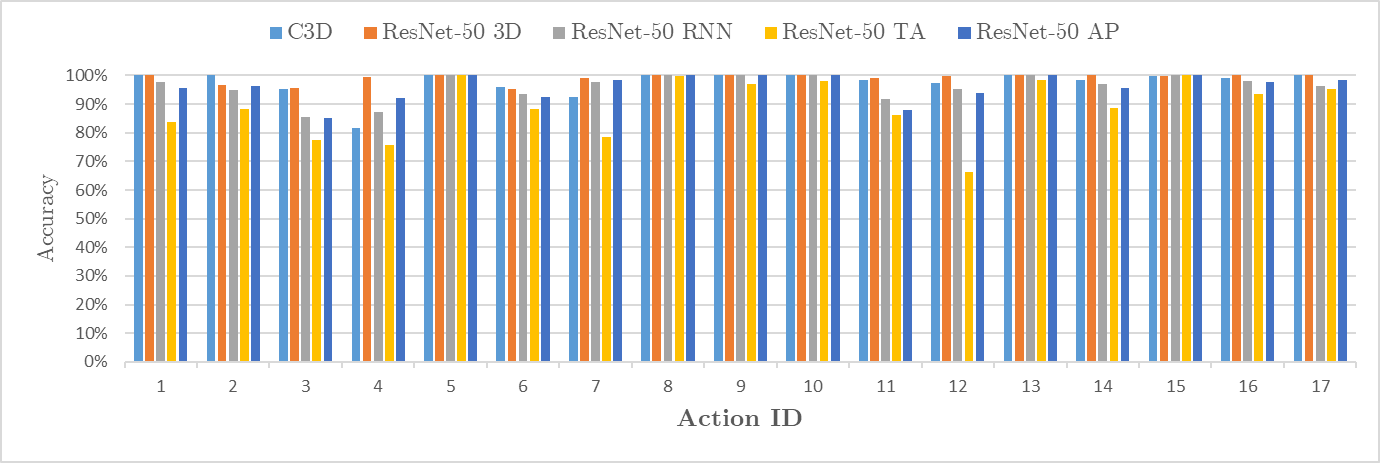
\includegraphics[width=1.0\linewidth]{figs/pc-MvDA_confusion_muhavi.png}
        \caption{Comparison of accuracy on each action class using different deep features combined with pc-MvDA.}
        %\vspace{-0.3cm}
        \label{fig:pc-MvDA_confusion_muhavi}
    \end{figure}

    Table \ref{tab:sota_muhavi} compares the best investigated combination of ResNet-50 3D and pc-MvDA with state-of-the-art frameworks. The comparison is for reference only because of aforementioned difference in setup of number of views and cross validation scheme.

    \begin{table}[htbp]
    \centering
    \caption{Comparison of the proposed methods with SOTA methods on MuHAVi dataset according to the second evaluation protocol.}
    \resizebox{0.7\textwidth}{!}{
    \begin{tabular}{|c|c|c|}
    \hline
    Methods                                                   & Cross-view & Multi-view \\ \hline
    Wu et al. \cite{wu2012view}                               & N/A       & 94.5     \\ \hline
    Zheng et al. \cite{zheng2016cross}                        & 94.88     & 99.8     \\ \hline
    Liu et al. \cite{liu2018learning}                         & N/A       & 91.2     \\ \hline
    Liu et al. \cite{liu2018hierarchically}                   & 99.91     & 99.8     \\ \hline
    Proposed method (ResNet-50 3D + pc-MvDA) \protect\footnotemark              & 99.90     & 99.88    \\ \hline
    \end{tabular}}
    \label{tab:sota_muhavi}
    \end{table}
    \footnotetext{Results when choosing only 4 views Camera 1, Camera 3, Camera 4 and Camera 6 following the other works.}

    %!TEX root = ../../../main.tex

\subsection{Experimental results on MICAGes dataset}

    \paragraph{1) Cross-view validation:} It can be seen in Table.\ref{tab:mica_cross} that pc-MvDA outperforms in almost every cases. With the first protocol, the norm accuracy of pc-MvDA of 74.52\% surpasses that of MvDA-vc (72.12\%) by 2.4\% and that of MvDA (64.94\%) by a large margin of 9.58\%. Especially in case of C3D features, the proposed algorithm achieved 90.2\% recognition rate whereas MvDA returns only 67.13\%.

    \begin{table}[htbp]
    \centering
    \caption{Cross-view recognition comparison on MICAGes dataset.}
    \resizebox{0.8\textwidth}{!}{
    \begin{tabular}{|c|c|c|c|c|c|c|}
        \hline
        \multirow{2}{*}{Deep features}          & \multicolumn{3}{c|}{Protocol 1}          & \multicolumn{3}{c|}{Protocol 2}            \\ \cline{2-7} 
                                                & MvDA  & MvDA-vc        & pc-MvDA         & MvDA  & MvDA-vc        & pc-MvDA           \\ \hline
        \multicolumn{1}{|c|}{C3D}               & 67.13 & 85.98          & \textbf{90.20}  & 93.74 & 99.80          & \textbf{100}      \\ \hline
        \multicolumn{1}{|c|}{ResNet-50 3D}      & 94.91 & 95.25          & \textbf{95.62}  & 97.43 & \textbf{99.97} & 99.79             \\ \hline
        \multicolumn{1}{|c|}{ResNet-50 RNN}     & 58.01 & 61.64          & \textbf{64.13}  & 100   & 100            & 100               \\ \hline
        \multicolumn{1}{|c|}{ResNet-50 TA}      & 53.58 & \textbf{59.55} & 58.62           & 96.70 & 99.48          & \textbf{99.83}    \\ \hline
        \multicolumn{1}{|c|}{ResNet-50 AP}      & 51.07 & 58.19          & \textbf{64.04}  & 99.73 & \textbf{99.99} & 99.89             \\ \hline
    \end{tabular}}
    \label{tab:mica_cross}
    \end{table}

    %Table.\ref{tab:cross_feature_mica} compares all types of deep features regarding accuracy of the proposed algorithm. 
    The top ranking of features applies identically and radically proves the superiority of 3D convolution based clip-level feature extraction in video recognition: ResNet-50 3D at 95.62\% and C3D at 90.2\%. The rest are ResNet-50 RNN (64.13\%), ResNet-50 AP (64.04\%) and ResNet-50 TA (58.62\%). For the second protocol, MvDA-vc (99.85\%) and pc-MvDA (99.9\%) are nearly even in performance while MvDA achieved 97.52\%.

    \begin{table}[htbp]
    \centering
    \caption{Cross-view recognition results of different features on MICAGes dataset with pc-MvDA method. The result in the bracket are accuracies of using features C3D, ResNet-50 3D, ResNet-50 RNN, ResNet-50 TA, RestNet-50 AP respectively. Each row corresponds to training view (from view K1 to view K5). Each column corresponds to testing view (from view K1 to view K5).}
    \resizebox{\textwidth}{!}{\begin{tabular}{|c|c|c|c|c|c|}
        \hline
        \backslashbox{Training}{Testing} & K1 & K2 & K3 & K4 & K5 \\ \hline
        K1 & N/A & \begin{tabular}{@{}c@{}} (92.9, \textbf{95.5}, 69.4, \\ 63.9, 65.1) \end{tabular} & \begin{tabular}{@{}c@{}} (93.7, \textbf{98.0}, 79.1, \\ 75.8, 74.7) \end{tabular} & \begin{tabular}{@{}c@{}} (90.5, \textbf{97.6}, 64.5, \\ 68.8, 70.8) \end{tabular} & \begin{tabular}{@{}c@{}} (89.2, \textbf{92.6}, 56.0, \\ 43.7, 58.2) \end{tabular} \\ \hline       
        K2 & \begin{tabular}{@{}c@{}} (84.7, \textbf{94.6}, 51.3, \\ 41.4, 53.7) \end{tabular} & N/A & \begin{tabular}{@{}c@{}} (94.6, \textbf{97.6}, 78.9, \\ 75.4, 77.5) \end{tabular} & \begin{tabular}{@{}c@{}} (91.3, \textbf{97.6}, 64.4, \\ 68.5, 68.0) \end{tabular} & \begin{tabular}{@{}c@{}} (87.4, \textbf{92.7}, 56.1, \\ 42.0, 55.6) \end{tabular} \\ \hline       
        K3 & \begin{tabular}{@{}c@{}} (87.5, \textbf{94.9}, 51.9, \\ 43.6, 52.7) \end{tabular} & \begin{tabular}{@{}c@{}} (93.0, \textbf{95.5}, 70.1, \\ 64.7, 63.4) \end{tabular} & N/A & \begin{tabular}{@{}c@{}} (90.0, \textbf{97.6}, 63.2, \\ 62.6, 67.5) \end{tabular} & \begin{tabular}{@{}c@{}} (88.9, \textbf{92.2}, 57.2, \\ 41.8, 56.6) \end{tabular} \\ \hline       
        K4 & \begin{tabular}{@{}c@{}} (86.7, \textbf{94.7}, 50.8, \\ 48.9, 54.9) \end{tabular} & \begin{tabular}{@{}c@{}} (90.2, \textbf{95.5}, 71.5, \\ 68.2, 61.8) \end{tabular} & \begin{tabular}{@{}c@{}} (92.5, \textbf{98.0}, 81.0, \\ 76.0, 74.4) \end{tabular} & N/A & \begin{tabular}{@{}c@{}} (89.7, \textbf{92.3}, 54.3, \\ 44.9, 56.6) \end{tabular} \\ \hline       
        K5 & \begin{tabular}{@{}c@{}} (84.9, \textbf{94.9}, 48.4, \\ 41.5, 57.9) \end{tabular} & \begin{tabular}{@{}c@{}} (90.4, \textbf{95.5}, 72.6, \\ 64.1, 65.7) \end{tabular} & \begin{tabular}{@{}c@{}} (94.0, \textbf{97.8}, 79.1, \\ 72.5, 76.3) \end{tabular} & \begin{tabular}{@{}c@{}} (91.9, \textbf{97.3}, 62.7, \\ 64.1, 69.0) \end{tabular} & N/A \\ \hline
    \end{tabular}}
    \label{tab:cross_feature_mica}
    \end{table}

    \paragraph{2) Multi-view validation}: The multi-view recognition results in Table.\ref{tab:mica_multi} shows an almost alike trend for both protocols. In general, pc-MvDA is 8.95\% and 0.72\% higher in accuracy for protocol 1, and 2.75\% and 0.04\% for protocol 2, in comparison with MvDA and MvDA-pc respectively.

    % TODO
    In virtually every experiments of MICAGes and two earlier benchmark datasets, the proposed extension is superior. The average accuracies of pc-MvDA is, in comparison on protocol 1 (and protocol 2 resp.), 5.29\% (1.21\% resp.) higher than MvDA, 1.21\% (0.62\% resp.) better than MvDA-vc. Despite not being as intuitive and straightly intelligible as pairwise-covariance, the multi-view resemblance added in MvDA-vc achieved nearly the performance of pc-MvDA. However, this view-consistency can be easily splitted into pairwise terms and intergrated into the objective of pc-MvDA in future works for further analysis.

    \begin{table}[htbp]
    \centering
    \caption{Multi-view recognition comparison on MICAGes dataset.}
    \resizebox{0.8\textwidth}{!}{
    \begin{tabular}{|c|c|c|c|c|c|c|}
        \hline
        \multirow{2}{*}{Deep features}          & \multicolumn{3}{c|}{Protocol 1}          & \multicolumn{3}{c|}{Protocol2}                     \\ \cline{2-7} 
                                                & MvDA  & MvDA-vc        & pc-MvDA         & MvDA           & MvDA-vc       & pc-MvDA           \\ \hline
        \multicolumn{1}{|c|}{C3D}               & 68.31 & 87.70          & \textbf{89.99}  & 88.79          & 99.54         & \textbf{100}      \\ \hline
        \multicolumn{1}{|c|}{ResNet-50 3D}      & 95.32 & 95.26          & \textbf{95.54}  & \textbf{100}   & 99.96         & 99.80             \\ \hline
        \multicolumn{1}{|c|}{ResNet-50 RNN}     & 57.50 & 63.05          & \textbf{63.83}  & 99.90          & \textbf{100}  & 99.97             \\ \hline
        \multicolumn{1}{|c|}{ResNet-50 TA}      & 54.43 & \textbf{61.46} & 58.25           & 96.72          & 99.49         & \textbf{99.69}    \\ \hline
        \multicolumn{1}{|c|}{ResNet-50 AP}      & 50.93 & 60.20          & \textbf{63.66}  & \textbf{99.99} & 99.93         & 99.67             \\ \hline
    \end{tabular}}
    \label{tab:mica_multi}
    \end{table}

    In addition to the same propensity shown, MICAGes also reveals the robustness of 3D convolution to generate fine clustered private feature space because this dataset contains exclusively hand gestures, which take part in a relatively small region of the captured videos. ResNet-50 3D and C3D are predominant for discriminant common space construction and classification and distances other features (Figure \ref{fig:pc-MvDA_confusion_mica}).

    \begin{figure}[htbp]
        \centering
        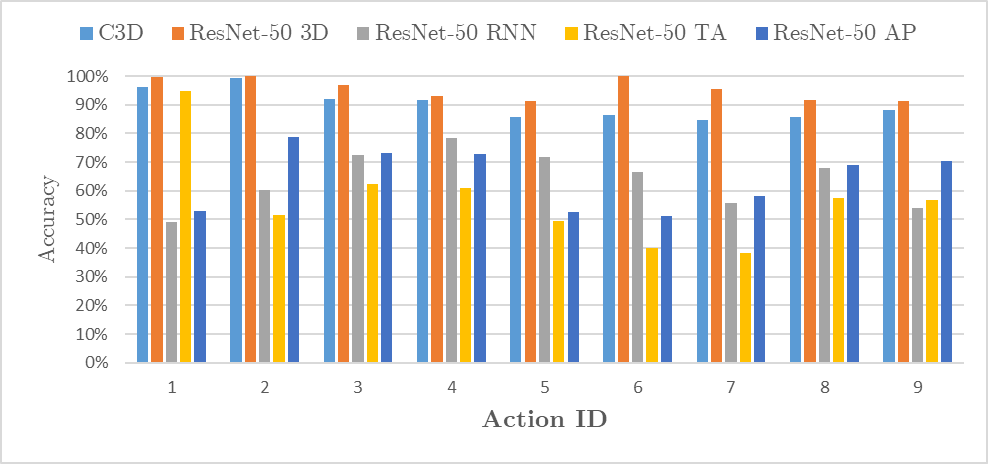
\includegraphics[width=0.8\linewidth]{figs/pc-MvDA_confusion_mica.png}
        \caption{Comparison of accuracy on each action class using different deep features combined with pc-MvDA on MICAGes dataset.}
        %\vspace{-0.3cm}
        \label{fig:pc-MvDA_confusion_mica}
    \end{figure}

    To better study the behavior of investigated multi-view analysis algorithms, t-SNE embedding of original private spaces, MvDA and pc-MvDA common space generated by protocol 1 are plotted in Figure \ref{fig:mica-tsne}. In these scatter plots, colors denote action classes, shapes as different views and train/test data are distinguished by border type. They explicitly denotes the surpassing capability of the proposed algorithm in finding a common space with prominent extra-class discrepancy. The data samples involved in training process are generally clustered in compact and separated blobs while testing data samples dissolve nearby. The better convergence of pc-MvDA compared to the baseline is usually only visible for harder features, whereas with the inputs of ResNet-50 3D features, which are already highly discriminated in private spaces, the improvement of pc-MvDA is negligible. Note that these illustrations of t-SNE embedding do not strictly depict an identical distribution of data.

    \begin{figure}[htbp]
        \centering
        \includegraphics[width=1\linewidth, height=0.6\pdfpageheight, keepaspectratio=false]{figs/mica-tsne.png}
        \caption{First column: private feature spaces stacked and embedded together in a same coordinate system; Second column: MvDA common space; Third column: pc-MvDA common space.}
        %\vspace{-0.3cm}
        \label{fig:mica-tsne}
    \end{figure}


    %!TEX root = ../../../main.tex

\section{Experimental Results and Discussions} \label{sec:results}
    %!TEX root = ../../../main.tex

\subsection{Experimental results on IXMAS dataset}
    \paragraph{1) Cross-view validation:} In this experiment, we train on data from one view (training view) and testing on data from another view (testing view) then compute the accuracies for two evaluation protocols. Table \ref{tab:cross_p1_ixmas} shows comparative results of using different deep features (C3D, ResNet-50 3D, ResNet-50 RNN, ResNet-50 TA, ResNet-50 AP) and multi-view discriminant analysis techniques (MvDA, MvDA-vc and our proposed pc-MvDA). 

    With the first evaluation protocol, the proposed pc-MvDA, when combined with deep features, gives mostly best accuracy for both evaluation protocols. With C3D features, accuracy by pc-MvDA (88.43\%) is 6.6\% higher than MvDA (81.84\%). pc-MvDA is even better than MvDA-vc (2.87\%). pc-MvDA achieved higher accuracy (about 6\% higher) than MvDA and MvDA-vc with ResNet-50 TA and ResNet-50 AP features. In average, pc-MvDA is 3.09\% higher than MvDA and 1.4\% higher than MvDA-vc.
    
    \begin{table}[htbp]
    \centering
    \caption{Cross-view recognition comparison on IXMAS dataset.}
    \resizebox{0.8\textwidth}{!}{
    \begin{tabular}{|l|c|c|c|c|c|c|}
        \hline
        \multirow{2}{*}{Deep features}          & \multicolumn{3}{c|}{Protocol 1}   & \multicolumn{3}{c|}{Protocol 2}           \\ \cline{2-7} 
                                                & MvDA  & MvDA-vc & pc-MvDA         & MvDA  & MvDA-vc        & pc-MvDA          \\ \hline
        \multicolumn{1}{|c|}{C3D}               & 81.84 & 85.56   & \textbf{88.43}  & 96.54 & 99.29          & \textbf{99.98}   \\ \hline
        \multicolumn{1}{|c|}{ResNet-50 3D}      & 91.25 & 92.19   & \textbf{92.89}  & 97.30 & \textbf{99.73} & 99.65            \\ \hline
        \multicolumn{1}{|c|}{ResNet-50 RNN}     & 75.51 & 76.12   & \textbf{76.54}  & 99.99 & 99.71          & \textbf{100}     \\ \hline
        \multicolumn{1}{|c|}{ResNet-50 TA}      & 79.44 & 80.58   & \textbf{82.05}  & 99.33 & 99.34          & \textbf{99.84}   \\ \hline
        \multicolumn{1}{|c|}{ResNet-50 AP}      & 77.00 & 79.04   & \textbf{80.58}  & 99.68 & 99.81          & \textbf{99.92}   \\ \hline
    \end{tabular}}
    \label{tab:cross_p1_ixmas}
    \end{table}

    For the second evaluation protocol, pc-MvDA almost always keeps better performance compared to MvDA and MvDA-vc. The recognition accuracy scores obtained by both pc-MvDA and MvDA-vc are nearly 100\% for every kind of deep features. With C3D features and ResNet-50 3D features, pc-MvDA is 99.98\% and 99.65\%, which is 3.44\% and 2.35\% higher than the orginal MvDA (96.54\% and 97.3\%) respectively. In average, pc-MvDA is 1.31\% better than MvDA and 0.3\% better than MvDA-vc. 

    In terms of deep features, with the first evaluation protocol, ResNet-50 3D gives the best accuracy (92.89\%) following by C3D (88.43\%), ResNet-50 TA (82.05\%), ResNet-50 AP (80.58\%). The lowest accuracy obtained by ResNet-50 RNN is only 76.54\%. It shows that ResNet-50 3D produces the most discriminative feature space. %Table \ref{tab:cross_feature_ixmas} shows comparative results when using pc-MvDA method with different deep features regarding pairwise views. 

    \begin{table}[htbp]
    \centering
    \caption{Cross-view recognition results of different features on IXMAS dataset with pc-MvDA method. The result in the bracket are accuracies of using features C3D, ResNet-50 3D, ResNet-50 RNN, ResNet-50 TA, Restnet-50 AP respectively. Each row corresponds to training view (from view C0 to view C3). Each column corresponds to testing view (from view C0 to view C3).}
    \resizebox{\textwidth}{!}{\begin{tabular}{|c|c|c|c|c|}
        \hline
        \backslashbox{Training}{Testing} & C0 & C1 & C2 & C3 \\ \hline
        C0 & N/A & (90.7, \textbf{91.9}, 81.6, 84.6, 83.6) & (86.9, \textbf{93.9}, 78.0, 79.6, 78.1) & (89.9, \textbf{93.4}, 76.3, 82.8, 82.1) \\ \hline
        C1 & (86.6, \textbf{91.9}, 71.5, 81.1, 77.5) & N/A & (85.9, \textbf{94.2}, 78.6, 79.3, 80.3) & (88.9, \textbf{93.7}, 74.8, 82.3, 81.3) \\ \hline
        C2 & (87.6, \textbf{92.4}, 72.8, 81.8, 78.5) & (90.7, \textbf{91.7}, 80.6, 83.6, 82.6) & N/A & (89.4, \textbf{93.7}, 75.5, 82.3, 80.6) \\ \hline
        C3 & (87.6, \textbf{92.9}, 70.2, 82.1, 78.8) & (90.7, \textbf{91.2}, 81.6, 84.1, 82.8) & (86.4, \textbf{93.7}, 77.3, 80.6, 80.8) & N/A \\ \hline
    \end{tabular}}
    \label{tab:cross_feature_ixmas}
    \end{table}

    \paragraph{2) Multi-view validation} Table \ref{tab:ixmas_multi} shows multi-view recognition results. The conclusion is consistent with the case of cross-view evaluation: ResNet-50 3D is the best feature extractor. When it is combined with pc-MvDA, the framework gives the highest accuracy for the first protocol (92.82\%), following by C3D (88.19\%), ResNet-50 TA (81.49\%), ResNet-50 AP(80.43\%), and ResNet-50 RNN (76.47\%). Both MvA algorithms give similar accuracies for the second evaluation protocols (nearly 100\%). Again, pc-MvDA enhances the performance of MvDA by 2.43\% for the first protocol and 0.83\% for the second protocol. It only gives slightly better result than MvDA-vc (0.83\% for the first protocol and 0.74\% for the second protocol). 

    \begin{table}[htbp]
    \centering
    \caption{Multi-view recognition comparison on IXMAS dataset.}
    \resizebox{0.7\textwidth}{!}{\begin{tabular}{|c|c|c|c|c|c|c|}
        \hline
        \multirow{2}{*}{Deep features}          & \multicolumn{3}{c|}{Protocol 1}   & \multicolumn{3}{c|}{Protocol2}                    \\ \cline{2-7} 
                                                & MvDA  & MvDA-vc & pc-MvDA         & MvDA           & MvDA-vc        & pc-MvDA         \\ \hline
        \multicolumn{1}{|c|}{C3D}               & 86.93 & 87.04   & \textbf{88.19}  & \textbf{99.99} & 99.44          & \textbf{99.98}  \\ \hline
        \multicolumn{1}{|c|}{ResNet-50 3D}      & 91.84 & 92.33   & \textbf{92.82}  & \textbf{100}   & 99.80          & 99,67           \\ \hline
        \multicolumn{1}{|c|}{ResNet-50 RNN}     & 72.44 & 75.95   & \textbf{76.47}  & 99.34          & \textbf{99.97} & \textbf{99.96}  \\ \hline
        \multicolumn{1}{|c|}{ResNet-50 TA}      & 76.74 & 81.01   & \textbf{81.49}  & 95.80          & 98.25          & \textbf{99.79}  \\ \hline
        \multicolumn{1}{|c|}{ResNet-50 AP}      & 79.28 & 78.93   & \textbf{80.43}  & \textbf{100}   & 98.11          & 99.85           \\ \hline
    \end{tabular}}
    \label{tab:ixmas_multi}
    \end{table}

    Figure \ref{fig:pc-MvDA_confusion_ixmas} compares the performance of feature extractors regarding each action class in multi-view evaluation scheme combined with the first evaluation protocol. There are clear margins between the performance of ResNet-50 3D and followed by C3D with other types of deep features, especially in harder actions (the first class to the third class and the eighth class to the eleventh class). These actions (check watch, cross arm, scratch head, wave, punch, kick, point) involve the most part static pose of the body and only movement of limbs, whereas other actions 4 - sit down, 5 - get up, 6 - turn around, 7 - walk and 12 - pickup include movement of the whole body and are easier to be recognized. This suggests that 3D convolution can better deal with small difference of movement in action images, which in turn generates a much more classification-ready feature space for latter stage of recognition.

    \begin{figure}[htbp]
        \centering
        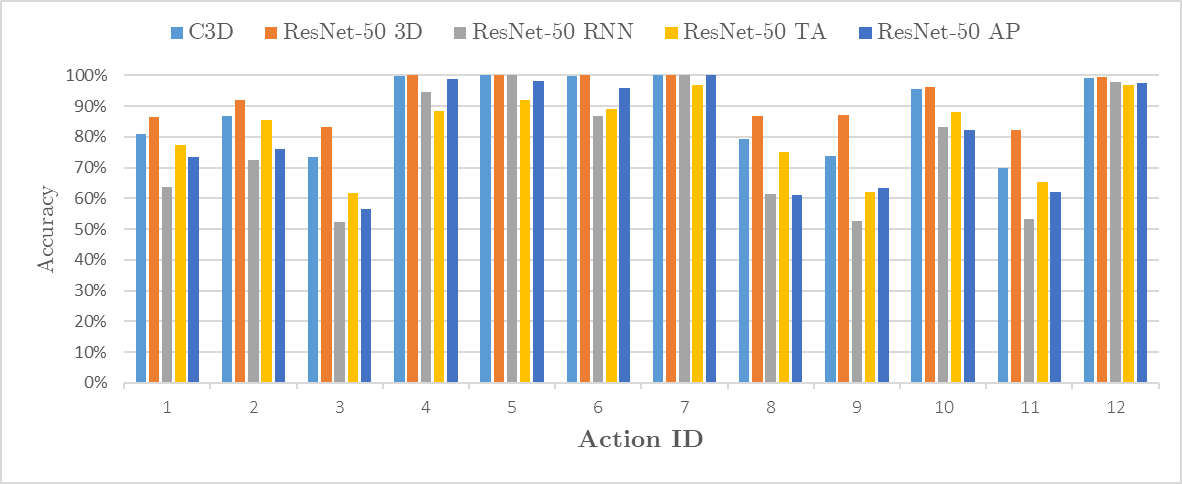
\includegraphics[width=0.8\linewidth]{figs/pc-MvDA_confusion_ixmas.png}
        \caption{Comparison of accuracy on each action class using different deep features combined with pc-MvDA on IXMAS dataset.}
        %\vspace{-0.3cm}
        \label{fig:pc-MvDA_confusion_ixmas}
    \end{figure}

    Table \ref{tab:sota_ixmas} compares the best combination of ResNet-50 3D and pc-MvDA with state-of-the-art frameworks. The comparison is for reference only because in other works, low-level hand-crafted video representation is used as private features and train-test strategy is leave-one-class out, which is not applicable to supervised deep feature extractors in this work. However, the results are still commensurable. % in circumstances where supervised approaches are adopted.
    % TODO - High priority

    \begin{table}[htbp]
    \centering
    \caption{Comparison of proposed methods with SOTA methods on IXMAS dataset according to the second evaluation protocol.}
    \resizebox{0.7\textwidth}{!}{
    \begin{tabular}{|c|c|c|}
    \hline
    Methods                                                              & Cross-view & Multi-view \\ \hline
    Liu et al. \cite{liu2011cross}                                   & 76.32      & N/A       \\ \hline
    Zheng et al. \cite{zheng2012cross}                               & 95.1       & 99.32     \\ \hline
    Zheng et al. \cite{zheng2016cross}                               & 97.8       & 99.4      \\ \hline
    Kong et al. \cite{kong2017deeply}                                & 99.92      & 100       \\ \hline
    Ulhaq et al. \cite{ulhaq2017space}                               & 66.82      & 92.47     \\ \hline
    Zhang et al. \cite{zhang2018cross}                               & 84.1       & N/A        \\ \hline
    Liu et al. \cite{liu2018learning}                                & N/A        & 90.3     \\ \hline
    Liu et al. \cite{liu2018hierarchically}                          & 99.95      & 99.67     \\ \hline
    Proposed method (ResNet-50 3D + pc-MvDA)                     & 99.67      & 99.65       \\ \hline
    \end{tabular}}
    \label{tab:sota_ixmas}
    \end{table}

    %!TEX root = ../../../main.tex

\subsection{Experimental results on MuHAVi dataset}
    \paragraph{1) Cross-view validation:} Table.\ref{tab:muhavi_cross} illustrates cross-view recognition results. The proposed pc-MvDA consistently produces a better average accuracy of around 96.19\% for protocol 1, approximately 4.55\% and 1.51\% higher than that of MvDA (91.64\%) and MvDA-vc (94.67\%) respectively.

    \begin{table}[htbp]
    \centering
    \caption{Cross-view recognition comparison on MuHAVi dataset.}
    \resizebox{0.8\textwidth}{!}{
    \begin{tabular}{|c|c|c|c|c|c|c|}
        \hline
        \multirow{2}{*}{Deep features}          & \multicolumn{3}{c|}{Protocol 1}   & \multicolumn{3}{c|}{Protocol 2}           \\ \cline{2-7} 
                                                & MvDA  & MvDA-vc & pc-MvDA         & MvDA  & MvDA-vc        & pc-MvDA          \\ \hline
        \multicolumn{1}{|c|}{C3D}               & 92.85 & 95.15   & \textbf{97.65}  & 98.95 & 99.76          & \textbf{100}     \\ \hline
        \multicolumn{1}{|c|}{ResNet-50 3D}      & 97.94 & 99.15   & \textbf{99.18}  & 96.77 & \textbf{99.94} & \textbf{99.94}   \\ \hline
        \multicolumn{1}{|c|}{ResNet-50 RNN}     & 95.54 & 95.14   & \textbf{96.18}  & 98.70 & 99.05          & \textbf{99.99}   \\ \hline
        \multicolumn{1}{|c|}{ResNet-50 TA}      & 85.80 & 88.95   & \textbf{91.12}  & 96.57 & 97.03          & \textbf{99.88}   \\ \hline
        \multicolumn{1}{|c|}{ResNet-50 AP}      & 86.09 & 94.98   & \textbf{96.82}  & 89.04 & 98.62          & \textbf{99.93}   \\ \hline
    \end{tabular}}
    \label{tab:muhavi_cross}
    \end{table}

    %Results in Table.\ref{tab:cross_feature_muhavi} show that our combination with ResNet-50 3D has the highest accuracies in almost every circumstances, even though both features coupled with our proposed pc-MvDA give satisfactory performance with all scores exceeding 91\%.

    \begin{table}[htbp]
    \centering
    \caption{Cross-view recognition results of different features on MuHAVi dataset with pc-MvDA method. The result in the bracket are accuracies of using features C3D, ResNet-50 3D, ResNet-50 RNN, ResNet-50 TA, ResNet-50 AP respectively. Each row corresponds to training view (from view C1 to view C7). Each column corresponds to testing view (from view C1 to view C7).}
    \resizebox{\textwidth}{!}{\begin{tabular}{|c|c|c|c|c|c|c|c|}
        \hline
        \backslashbox{Training}{Testing} & C1 & C2 & C3 & C4 & C5 & C6 & C7 \\ \hline
        C1 & N/A & \begin{tabular}{@{}c@{}} (96.1, \textbf{100}, 96.8, \\ 88.5, 98.5) \end{tabular} & \begin{tabular}{@{}c@{}} (98.6, \textbf{99.6}, 96.6, \\ 88.9, 96.3) \end{tabular} & \begin{tabular}{@{}c@{}} (98.6, \textbf{99.6}, 98.0, \\ 93.1, 98.2) \end{tabular} & \begin{tabular}{@{}c@{}} (97.7, \textbf{99.6}, 95.4, \\ 91.3, 96.1) \end{tabular} & \begin{tabular}{@{}c@{}} (97.7, \textbf{98.4}, 92.3, \\ 93.1, 96.3) \end{tabular} & \begin{tabular}{@{}c@{}} (98.2, \textbf{98.5}, 97.2, \\ 89.8, 97.1) \end{tabular} \\ \hline
        C2 & \begin{tabular}{@{}c@{}} (95.6, \textbf{99.0}, 95.2, \\ 91.3, 95.5) \end{tabular} & N/A & \begin{tabular}{@{}c@{}} (98.9, \textbf{99.6}, 96.9, \\ 90.3, 96.1) \end{tabular} & \begin{tabular}{@{}c@{}} (98.4, \textbf{99.6}, 97.6, \\ 92.6, 98.2) \end{tabular} & \begin{tabular}{@{}c@{}} (97.7, \textbf{99.6}, 95.4, \\ 90.9, 96.1) \end{tabular} & \begin{tabular}{@{}c@{}} (97.8, \textbf{98.4}, 92.7, \\ 93.6, 96.5) \end{tabular} & \begin{tabular}{@{}c@{}} (98.6, \textbf{99.0}, 97.4, \\ 90.6, 96.9) \end{tabular} \\ \hline
        C3 & \begin{tabular}{@{}c@{}} (96.1, \textbf{99.0}, 95.6, \\ 90.3, 95.1) \end{tabular} & \begin{tabular}{@{}c@{}} (97.0, \textbf{100}, 96.7, \\ 88.4, 97.8) \end{tabular} & N/A & \begin{tabular}{@{}c@{}} (98.1, \textbf{99.2}, 98.2, \\ 92.8, 98.2) \end{tabular} & \begin{tabular}{@{}c@{}} (97.9, \textbf{99.6}, 95.4, \\ 90.2, 95.6) \end{tabular} & \begin{tabular}{@{}c@{}} (97.9, \textbf{98.2}, 93.0, \\ 94.2, 96.5) \end{tabular} & \begin{tabular}{@{}c@{}} (97.8, \textbf{98.7}, 97.4, \\ 89.4, 97.6) \end{tabular} \\ \hline
        C4 & \begin{tabular}{@{}c@{}} (96.4, \textbf{98.8}, 95.4, \\ 89.6, 95.3) \end{tabular} & \begin{tabular}{@{}c@{}} (96.3, \textbf{100}, 96.6, \\ 91.0, 98.5) \end{tabular} & \begin{tabular}{@{}c@{}} (98.6, \textbf{99.6}, 97.3, \\ 89.5, 96.1) \end{tabular} & N/A & \begin{tabular}{@{}c@{}} (97.7, \textbf{99.4}, 95.6, \\ 91.3, 96.1) \end{tabular} & \begin{tabular}{@{}c@{}} (\textbf{98.4}, 98.0, 93.2, \\ 93.8, 95.6) \end{tabular} & \begin{tabular}{@{}c@{}} (97.7, \textbf{98.7}, 97.4, \\ 91.3, 96.7) \end{tabular} \\ \hline
        C5 & \begin{tabular}{@{}c@{}} (95.9, \textbf{99.0}, 95.6, \\ 91.3, 95.5) \end{tabular} & \begin{tabular}{@{}c@{}} (96.6, \textbf{100}, 97.1, \\ 89.9, 98.3) \end{tabular} & \begin{tabular}{@{}c@{}} (98.8, \textbf{99.4}, 96.8, \\ 90.7, 96.1) \end{tabular} & \begin{tabular}{@{}c@{}} (98.4, \textbf{99.6}, 98.0, \\ 92.1, 97.6) \end{tabular} & N/A & \begin{tabular}{@{}c@{}} (97.9, \textbf{98.2}, 93.4, \\ 94.4, 96.8) \end{tabular} & \begin{tabular}{@{}c@{}} (98.0, \textbf{98.7}, 96.9, \\ 89.0, 97.8) \end{tabular} \\ \hline
        C6 & \begin{tabular}{@{}c@{}} (95.8, \textbf{99.0}, 95.8, \\ 90.3, 95.0) \end{tabular} & \begin{tabular}{@{}c@{}} (97.0, \textbf{100}, 97.6, \\ 89.7, 98.5) \end{tabular} & \begin{tabular}{@{}c@{}} (98.8, \textbf{99.6}, 96.9, \\ 88.7, 96.1) \end{tabular} & \begin{tabular}{@{}c@{}} (98.4, \textbf{99.4}, 98.0, \\ 92.8, 98.2) \end{tabular} & \begin{tabular}{@{}c@{}} (97.5, \textbf{99.6}, 95.9, \\ 91.2, 95.5) \end{tabular} & N/A & \begin{tabular}{@{}c@{}} (98.2, \textbf{99.0}, 97.2, \\ 90.7, 97.4) \end{tabular} \\ \hline
        C7 & \begin{tabular}{@{}c@{}} (96.2, \textbf{98.8}, 95.7, \\ 91.5, 96.2) \end{tabular} & \begin{tabular}{@{}c@{}} (96.4, \textbf{100}, 97.5, \\ 90.3, 98.5) \end{tabular} & \begin{tabular}{@{}c@{}} (98.4, \textbf{99.0}, 97.3, \\ 90.0, 96.7) \end{tabular} & \begin{tabular}{@{}c@{}} (\textbf{98.8}, 98.8, 98.2, \\ 92.8, 98.0) \end{tabular} & \begin{tabular}{@{}c@{}} (97.5, \textbf{99.8}, 95.9, \\ 91.5, 95.9) \end{tabular} & \begin{tabular}{@{}c@{}} (\textbf{98.9}, 98.2, 92.8, \\ 93.9, 97.1) \end{tabular} & N/A \\ \hline
    \end{tabular}}
    \label{tab:cross_feature_muhavi}
    \end{table}

    \paragraph{2) Multi-view validation}: Table.\ref{tab:muhavi_multi} shows multi-view recognition results. The first protocol shows very close capability of MvDA-vc and pc-MvDA at 95.54\% and 95.83\% whereas MvDA is about 3\% behind at 92.7\%. For the second protocol, our variant exceeds MvDA by 2.21\% and MvDA-vc by 1.49\%. The near perfect results of the second protocol give us the same indication that it is not an inequitable method of comparison of MvA algorithms. 

    \begin{table}[htbp]
    \centering
    \caption{Multi-view recognition comparison on MuHAVi dataset.}
    \resizebox{0.8\textwidth}{!}{
    \begin{tabular}{|c|c|c|c|c|c|c|}
        \hline
        \multirow{2}{*}{Deep features}          & \multicolumn{3}{c|}{Protocol 1}                   & \multicolumn{3}{c|}{Protocol2}            \\ \cline{2-7} 
                                                & MvDA           & MvDA-vc        & pc-MvDA         & MvDA           & MvDA-vc & pc-MvDA        \\ \hline
        \multicolumn{1}{|c|}{C3D}               & 81.80          & 96.05          & \textbf{97.37}  & 88.39          & 99.61   & \textbf{100}   \\ \hline
        \multicolumn{1}{|c|}{ResNet-50 3D}      & 99.07          & 99.12          & \textbf{99.15}  & \textbf{99.98} & 99.96   & 99.89          \\ \hline
        \multicolumn{1}{|c|}{ResNet-50 RNN}     & \textbf{96.18} & 95.55          & 95.97           & \textbf{100}   & 99.00   & 99.98          \\ \hline
        \multicolumn{1}{|c|}{ResNet-50 TA}      & \textbf{90.45} & 89.73          & 90.22           & \textbf{99.92} & 98.17   & 99.72          \\ \hline
        \multicolumn{1}{|c|}{ResNet-50 AP}      & 96.01          & \textbf{96.75} & 96.42           & \textbf{100}   & 95.13   & 99.68          \\ \hline
    \end{tabular}}
    \label{tab:muhavi_multi}
    \end{table}

    Figure \ref{fig:pc-MvDA_confusion_muhavi} compares the performance of feature extractors regarding each action class in multi-view evaluation scheme combined with protocol 1. For this dataset, ResNet-50 3D persistently yields out-standing performance while ResNet-50 TA has the worst recognition rates in all action classes.

    \begin{figure}[htbp]
        \centering
        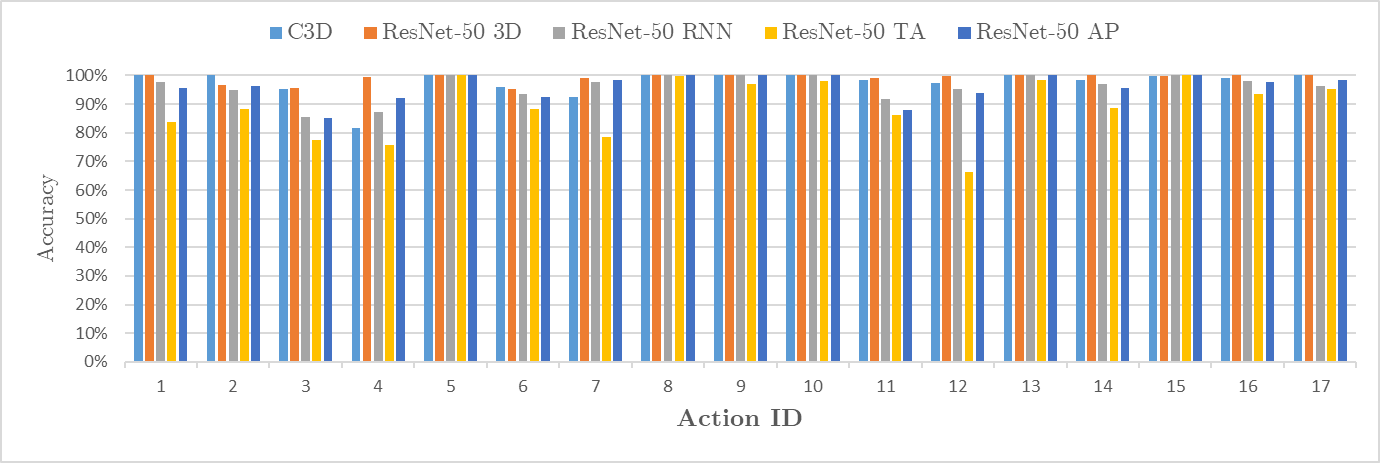
\includegraphics[width=1.0\linewidth]{figs/pc-MvDA_confusion_muhavi.png}
        \caption{Comparison of accuracy on each action class using different deep features combined with pc-MvDA.}
        %\vspace{-0.3cm}
        \label{fig:pc-MvDA_confusion_muhavi}
    \end{figure}

    Table \ref{tab:sota_muhavi} compares the best investigated combination of ResNet-50 3D and pc-MvDA with state-of-the-art frameworks. The comparison is for reference only because of aforementioned difference in setup of number of views and cross validation scheme.

    \begin{table}[htbp]
    \centering
    \caption{Comparison of the proposed methods with SOTA methods on MuHAVi dataset according to the second evaluation protocol.}
    \resizebox{0.7\textwidth}{!}{
    \begin{tabular}{|c|c|c|}
    \hline
    Methods                                                   & Cross-view & Multi-view \\ \hline
    Wu et al. \cite{wu2012view}                               & N/A       & 94.5     \\ \hline
    Zheng et al. \cite{zheng2016cross}                        & 94.88     & 99.8     \\ \hline
    Liu et al. \cite{liu2018learning}                         & N/A       & 91.2     \\ \hline
    Liu et al. \cite{liu2018hierarchically}                   & 99.91     & 99.8     \\ \hline
    Proposed method (ResNet-50 3D + pc-MvDA) \protect\footnotemark              & 99.90     & 99.88    \\ \hline
    \end{tabular}}
    \label{tab:sota_muhavi}
    \end{table}
    \footnotetext{Results when choosing only 4 views Camera 1, Camera 3, Camera 4 and Camera 6 following the other works.}

    %!TEX root = ../../../main.tex

\subsection{Experimental results on MICAGes dataset}

    \paragraph{1) Cross-view validation:} It can be seen in Table.\ref{tab:mica_cross} that pc-MvDA outperforms in almost every cases. With the first protocol, the norm accuracy of pc-MvDA of 74.52\% surpasses that of MvDA-vc (72.12\%) by 2.4\% and that of MvDA (64.94\%) by a large margin of 9.58\%. Especially in case of C3D features, the proposed algorithm achieved 90.2\% recognition rate whereas MvDA returns only 67.13\%.

    \begin{table}[htbp]
    \centering
    \caption{Cross-view recognition comparison on MICAGes dataset.}
    \resizebox{0.8\textwidth}{!}{
    \begin{tabular}{|c|c|c|c|c|c|c|}
        \hline
        \multirow{2}{*}{Deep features}          & \multicolumn{3}{c|}{Protocol 1}          & \multicolumn{3}{c|}{Protocol 2}            \\ \cline{2-7} 
                                                & MvDA  & MvDA-vc        & pc-MvDA         & MvDA  & MvDA-vc        & pc-MvDA           \\ \hline
        \multicolumn{1}{|c|}{C3D}               & 67.13 & 85.98          & \textbf{90.20}  & 93.74 & 99.80          & \textbf{100}      \\ \hline
        \multicolumn{1}{|c|}{ResNet-50 3D}      & 94.91 & 95.25          & \textbf{95.62}  & 97.43 & \textbf{99.97} & 99.79             \\ \hline
        \multicolumn{1}{|c|}{ResNet-50 RNN}     & 58.01 & 61.64          & \textbf{64.13}  & 100   & 100            & 100               \\ \hline
        \multicolumn{1}{|c|}{ResNet-50 TA}      & 53.58 & \textbf{59.55} & 58.62           & 96.70 & 99.48          & \textbf{99.83}    \\ \hline
        \multicolumn{1}{|c|}{ResNet-50 AP}      & 51.07 & 58.19          & \textbf{64.04}  & 99.73 & \textbf{99.99} & 99.89             \\ \hline
    \end{tabular}}
    \label{tab:mica_cross}
    \end{table}

    %Table.\ref{tab:cross_feature_mica} compares all types of deep features regarding accuracy of the proposed algorithm. 
    The top ranking of features applies identically and radically proves the superiority of 3D convolution based clip-level feature extraction in video recognition: ResNet-50 3D at 95.62\% and C3D at 90.2\%. The rest are ResNet-50 RNN (64.13\%), ResNet-50 AP (64.04\%) and ResNet-50 TA (58.62\%). For the second protocol, MvDA-vc (99.85\%) and pc-MvDA (99.9\%) are nearly even in performance while MvDA achieved 97.52\%.

    \begin{table}[htbp]
    \centering
    \caption{Cross-view recognition results of different features on MICAGes dataset with pc-MvDA method. The result in the bracket are accuracies of using features C3D, ResNet-50 3D, ResNet-50 RNN, ResNet-50 TA, RestNet-50 AP respectively. Each row corresponds to training view (from view K1 to view K5). Each column corresponds to testing view (from view K1 to view K5).}
    \resizebox{\textwidth}{!}{\begin{tabular}{|c|c|c|c|c|c|}
        \hline
        \backslashbox{Training}{Testing} & K1 & K2 & K3 & K4 & K5 \\ \hline
        K1 & N/A & \begin{tabular}{@{}c@{}} (92.9, \textbf{95.5}, 69.4, \\ 63.9, 65.1) \end{tabular} & \begin{tabular}{@{}c@{}} (93.7, \textbf{98.0}, 79.1, \\ 75.8, 74.7) \end{tabular} & \begin{tabular}{@{}c@{}} (90.5, \textbf{97.6}, 64.5, \\ 68.8, 70.8) \end{tabular} & \begin{tabular}{@{}c@{}} (89.2, \textbf{92.6}, 56.0, \\ 43.7, 58.2) \end{tabular} \\ \hline       
        K2 & \begin{tabular}{@{}c@{}} (84.7, \textbf{94.6}, 51.3, \\ 41.4, 53.7) \end{tabular} & N/A & \begin{tabular}{@{}c@{}} (94.6, \textbf{97.6}, 78.9, \\ 75.4, 77.5) \end{tabular} & \begin{tabular}{@{}c@{}} (91.3, \textbf{97.6}, 64.4, \\ 68.5, 68.0) \end{tabular} & \begin{tabular}{@{}c@{}} (87.4, \textbf{92.7}, 56.1, \\ 42.0, 55.6) \end{tabular} \\ \hline       
        K3 & \begin{tabular}{@{}c@{}} (87.5, \textbf{94.9}, 51.9, \\ 43.6, 52.7) \end{tabular} & \begin{tabular}{@{}c@{}} (93.0, \textbf{95.5}, 70.1, \\ 64.7, 63.4) \end{tabular} & N/A & \begin{tabular}{@{}c@{}} (90.0, \textbf{97.6}, 63.2, \\ 62.6, 67.5) \end{tabular} & \begin{tabular}{@{}c@{}} (88.9, \textbf{92.2}, 57.2, \\ 41.8, 56.6) \end{tabular} \\ \hline       
        K4 & \begin{tabular}{@{}c@{}} (86.7, \textbf{94.7}, 50.8, \\ 48.9, 54.9) \end{tabular} & \begin{tabular}{@{}c@{}} (90.2, \textbf{95.5}, 71.5, \\ 68.2, 61.8) \end{tabular} & \begin{tabular}{@{}c@{}} (92.5, \textbf{98.0}, 81.0, \\ 76.0, 74.4) \end{tabular} & N/A & \begin{tabular}{@{}c@{}} (89.7, \textbf{92.3}, 54.3, \\ 44.9, 56.6) \end{tabular} \\ \hline       
        K5 & \begin{tabular}{@{}c@{}} (84.9, \textbf{94.9}, 48.4, \\ 41.5, 57.9) \end{tabular} & \begin{tabular}{@{}c@{}} (90.4, \textbf{95.5}, 72.6, \\ 64.1, 65.7) \end{tabular} & \begin{tabular}{@{}c@{}} (94.0, \textbf{97.8}, 79.1, \\ 72.5, 76.3) \end{tabular} & \begin{tabular}{@{}c@{}} (91.9, \textbf{97.3}, 62.7, \\ 64.1, 69.0) \end{tabular} & N/A \\ \hline
    \end{tabular}}
    \label{tab:cross_feature_mica}
    \end{table}

    \paragraph{2) Multi-view validation}: The multi-view recognition results in Table.\ref{tab:mica_multi} shows an almost alike trend for both protocols. In general, pc-MvDA is 8.95\% and 0.72\% higher in accuracy for protocol 1, and 2.75\% and 0.04\% for protocol 2, in comparison with MvDA and MvDA-pc respectively.

    % TODO
    In virtually every experiments of MICAGes and two earlier benchmark datasets, the proposed extension is superior. The average accuracies of pc-MvDA is, in comparison on protocol 1 (and protocol 2 resp.), 5.29\% (1.21\% resp.) higher than MvDA, 1.21\% (0.62\% resp.) better than MvDA-vc. Despite not being as intuitive and straightly intelligible as pairwise-covariance, the multi-view resemblance added in MvDA-vc achieved nearly the performance of pc-MvDA. However, this view-consistency can be easily splitted into pairwise terms and intergrated into the objective of pc-MvDA in future works for further analysis.

    \begin{table}[htbp]
    \centering
    \caption{Multi-view recognition comparison on MICAGes dataset.}
    \resizebox{0.8\textwidth}{!}{
    \begin{tabular}{|c|c|c|c|c|c|c|}
        \hline
        \multirow{2}{*}{Deep features}          & \multicolumn{3}{c|}{Protocol 1}          & \multicolumn{3}{c|}{Protocol2}                     \\ \cline{2-7} 
                                                & MvDA  & MvDA-vc        & pc-MvDA         & MvDA           & MvDA-vc       & pc-MvDA           \\ \hline
        \multicolumn{1}{|c|}{C3D}               & 68.31 & 87.70          & \textbf{89.99}  & 88.79          & 99.54         & \textbf{100}      \\ \hline
        \multicolumn{1}{|c|}{ResNet-50 3D}      & 95.32 & 95.26          & \textbf{95.54}  & \textbf{100}   & 99.96         & 99.80             \\ \hline
        \multicolumn{1}{|c|}{ResNet-50 RNN}     & 57.50 & 63.05          & \textbf{63.83}  & 99.90          & \textbf{100}  & 99.97             \\ \hline
        \multicolumn{1}{|c|}{ResNet-50 TA}      & 54.43 & \textbf{61.46} & 58.25           & 96.72          & 99.49         & \textbf{99.69}    \\ \hline
        \multicolumn{1}{|c|}{ResNet-50 AP}      & 50.93 & 60.20          & \textbf{63.66}  & \textbf{99.99} & 99.93         & 99.67             \\ \hline
    \end{tabular}}
    \label{tab:mica_multi}
    \end{table}

    In addition to the same propensity shown, MICAGes also reveals the robustness of 3D convolution to generate fine clustered private feature space because this dataset contains exclusively hand gestures, which take part in a relatively small region of the captured videos. ResNet-50 3D and C3D are predominant for discriminant common space construction and classification and distances other features (Figure \ref{fig:pc-MvDA_confusion_mica}).

    \begin{figure}[htbp]
        \centering
        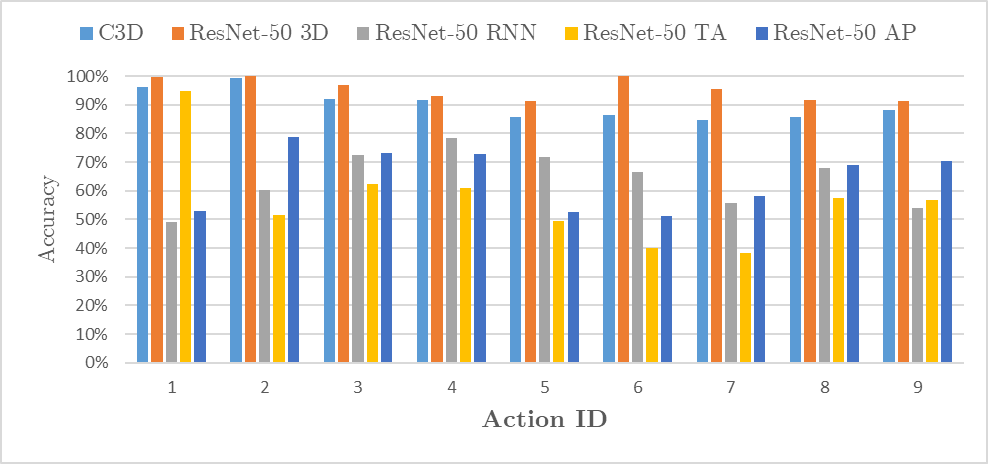
\includegraphics[width=0.8\linewidth]{figs/pc-MvDA_confusion_mica.png}
        \caption{Comparison of accuracy on each action class using different deep features combined with pc-MvDA on MICAGes dataset.}
        %\vspace{-0.3cm}
        \label{fig:pc-MvDA_confusion_mica}
    \end{figure}

    To better study the behavior of investigated multi-view analysis algorithms, t-SNE embedding of original private spaces, MvDA and pc-MvDA common space generated by protocol 1 are plotted in Figure \ref{fig:mica-tsne}. In these scatter plots, colors denote action classes, shapes as different views and train/test data are distinguished by border type. They explicitly denotes the surpassing capability of the proposed algorithm in finding a common space with prominent extra-class discrepancy. The data samples involved in training process are generally clustered in compact and separated blobs while testing data samples dissolve nearby. The better convergence of pc-MvDA compared to the baseline is usually only visible for harder features, whereas with the inputs of ResNet-50 3D features, which are already highly discriminated in private spaces, the improvement of pc-MvDA is negligible. Note that these illustrations of t-SNE embedding do not strictly depict an identical distribution of data.

    \begin{figure}[htbp]
        \centering
        \includegraphics[width=1\linewidth, height=0.6\pdfpageheight, keepaspectratio=false]{figs/mica-tsne.png}
        \caption{First column: private feature spaces stacked and embedded together in a same coordinate system; Second column: MvDA common space; Third column: pc-MvDA common space.}
        %\vspace{-0.3cm}
        \label{fig:mica-tsne}
    \end{figure}


    %!TEX root = ../../../main.tex

\section{Experimental Results and Discussions} \label{sec:results}
    %!TEX root = ../../../main.tex

\subsection{Experimental results on IXMAS dataset}
    \paragraph{1) Cross-view validation:} In this experiment, we train on data from one view (training view) and testing on data from another view (testing view) then compute the accuracies for two evaluation protocols. Table \ref{tab:cross_p1_ixmas} shows comparative results of using different deep features (C3D, ResNet-50 3D, ResNet-50 RNN, ResNet-50 TA, ResNet-50 AP) and multi-view discriminant analysis techniques (MvDA, MvDA-vc and our proposed pc-MvDA). 

    With the first evaluation protocol, the proposed pc-MvDA, when combined with deep features, gives mostly best accuracy for both evaluation protocols. With C3D features, accuracy by pc-MvDA (88.43\%) is 6.6\% higher than MvDA (81.84\%). pc-MvDA is even better than MvDA-vc (2.87\%). pc-MvDA achieved higher accuracy (about 6\% higher) than MvDA and MvDA-vc with ResNet-50 TA and ResNet-50 AP features. In average, pc-MvDA is 3.09\% higher than MvDA and 1.4\% higher than MvDA-vc.
    
    \begin{table}[htbp]
    \centering
    \caption{Cross-view recognition comparison on IXMAS dataset.}
    \resizebox{0.8\textwidth}{!}{
    \begin{tabular}{|l|c|c|c|c|c|c|}
        \hline
        \multirow{2}{*}{Deep features}          & \multicolumn{3}{c|}{Protocol 1}   & \multicolumn{3}{c|}{Protocol 2}           \\ \cline{2-7} 
                                                & MvDA  & MvDA-vc & pc-MvDA         & MvDA  & MvDA-vc        & pc-MvDA          \\ \hline
        \multicolumn{1}{|c|}{C3D}               & 81.84 & 85.56   & \textbf{88.43}  & 96.54 & 99.29          & \textbf{99.98}   \\ \hline
        \multicolumn{1}{|c|}{ResNet-50 3D}      & 91.25 & 92.19   & \textbf{92.89}  & 97.30 & \textbf{99.73} & 99.65            \\ \hline
        \multicolumn{1}{|c|}{ResNet-50 RNN}     & 75.51 & 76.12   & \textbf{76.54}  & 99.99 & 99.71          & \textbf{100}     \\ \hline
        \multicolumn{1}{|c|}{ResNet-50 TA}      & 79.44 & 80.58   & \textbf{82.05}  & 99.33 & 99.34          & \textbf{99.84}   \\ \hline
        \multicolumn{1}{|c|}{ResNet-50 AP}      & 77.00 & 79.04   & \textbf{80.58}  & 99.68 & 99.81          & \textbf{99.92}   \\ \hline
    \end{tabular}}
    \label{tab:cross_p1_ixmas}
    \end{table}

    For the second evaluation protocol, pc-MvDA almost always keeps better performance compared to MvDA and MvDA-vc. The recognition accuracy scores obtained by both pc-MvDA and MvDA-vc are nearly 100\% for every kind of deep features. With C3D features and ResNet-50 3D features, pc-MvDA is 99.98\% and 99.65\%, which is 3.44\% and 2.35\% higher than the orginal MvDA (96.54\% and 97.3\%) respectively. In average, pc-MvDA is 1.31\% better than MvDA and 0.3\% better than MvDA-vc. 

    In terms of deep features, with the first evaluation protocol, ResNet-50 3D gives the best accuracy (92.89\%) following by C3D (88.43\%), ResNet-50 TA (82.05\%), ResNet-50 AP (80.58\%). The lowest accuracy obtained by ResNet-50 RNN is only 76.54\%. It shows that ResNet-50 3D produces the most discriminative feature space. %Table \ref{tab:cross_feature_ixmas} shows comparative results when using pc-MvDA method with different deep features regarding pairwise views. 

    \begin{table}[htbp]
    \centering
    \caption{Cross-view recognition results of different features on IXMAS dataset with pc-MvDA method. The result in the bracket are accuracies of using features C3D, ResNet-50 3D, ResNet-50 RNN, ResNet-50 TA, Restnet-50 AP respectively. Each row corresponds to training view (from view C0 to view C3). Each column corresponds to testing view (from view C0 to view C3).}
    \resizebox{\textwidth}{!}{\begin{tabular}{|c|c|c|c|c|}
        \hline
        \backslashbox{Training}{Testing} & C0 & C1 & C2 & C3 \\ \hline
        C0 & N/A & (90.7, \textbf{91.9}, 81.6, 84.6, 83.6) & (86.9, \textbf{93.9}, 78.0, 79.6, 78.1) & (89.9, \textbf{93.4}, 76.3, 82.8, 82.1) \\ \hline
        C1 & (86.6, \textbf{91.9}, 71.5, 81.1, 77.5) & N/A & (85.9, \textbf{94.2}, 78.6, 79.3, 80.3) & (88.9, \textbf{93.7}, 74.8, 82.3, 81.3) \\ \hline
        C2 & (87.6, \textbf{92.4}, 72.8, 81.8, 78.5) & (90.7, \textbf{91.7}, 80.6, 83.6, 82.6) & N/A & (89.4, \textbf{93.7}, 75.5, 82.3, 80.6) \\ \hline
        C3 & (87.6, \textbf{92.9}, 70.2, 82.1, 78.8) & (90.7, \textbf{91.2}, 81.6, 84.1, 82.8) & (86.4, \textbf{93.7}, 77.3, 80.6, 80.8) & N/A \\ \hline
    \end{tabular}}
    \label{tab:cross_feature_ixmas}
    \end{table}

    \paragraph{2) Multi-view validation} Table \ref{tab:ixmas_multi} shows multi-view recognition results. The conclusion is consistent with the case of cross-view evaluation: ResNet-50 3D is the best feature extractor. When it is combined with pc-MvDA, the framework gives the highest accuracy for the first protocol (92.82\%), following by C3D (88.19\%), ResNet-50 TA (81.49\%), ResNet-50 AP(80.43\%), and ResNet-50 RNN (76.47\%). Both MvA algorithms give similar accuracies for the second evaluation protocols (nearly 100\%). Again, pc-MvDA enhances the performance of MvDA by 2.43\% for the first protocol and 0.83\% for the second protocol. It only gives slightly better result than MvDA-vc (0.83\% for the first protocol and 0.74\% for the second protocol). 

    \begin{table}[htbp]
    \centering
    \caption{Multi-view recognition comparison on IXMAS dataset.}
    \resizebox{0.7\textwidth}{!}{\begin{tabular}{|c|c|c|c|c|c|c|}
        \hline
        \multirow{2}{*}{Deep features}          & \multicolumn{3}{c|}{Protocol 1}   & \multicolumn{3}{c|}{Protocol2}                    \\ \cline{2-7} 
                                                & MvDA  & MvDA-vc & pc-MvDA         & MvDA           & MvDA-vc        & pc-MvDA         \\ \hline
        \multicolumn{1}{|c|}{C3D}               & 86.93 & 87.04   & \textbf{88.19}  & \textbf{99.99} & 99.44          & \textbf{99.98}  \\ \hline
        \multicolumn{1}{|c|}{ResNet-50 3D}      & 91.84 & 92.33   & \textbf{92.82}  & \textbf{100}   & 99.80          & 99,67           \\ \hline
        \multicolumn{1}{|c|}{ResNet-50 RNN}     & 72.44 & 75.95   & \textbf{76.47}  & 99.34          & \textbf{99.97} & \textbf{99.96}  \\ \hline
        \multicolumn{1}{|c|}{ResNet-50 TA}      & 76.74 & 81.01   & \textbf{81.49}  & 95.80          & 98.25          & \textbf{99.79}  \\ \hline
        \multicolumn{1}{|c|}{ResNet-50 AP}      & 79.28 & 78.93   & \textbf{80.43}  & \textbf{100}   & 98.11          & 99.85           \\ \hline
    \end{tabular}}
    \label{tab:ixmas_multi}
    \end{table}

    Figure \ref{fig:pc-MvDA_confusion_ixmas} compares the performance of feature extractors regarding each action class in multi-view evaluation scheme combined with the first evaluation protocol. There are clear margins between the performance of ResNet-50 3D and followed by C3D with other types of deep features, especially in harder actions (the first class to the third class and the eighth class to the eleventh class). These actions (check watch, cross arm, scratch head, wave, punch, kick, point) involve the most part static pose of the body and only movement of limbs, whereas other actions 4 - sit down, 5 - get up, 6 - turn around, 7 - walk and 12 - pickup include movement of the whole body and are easier to be recognized. This suggests that 3D convolution can better deal with small difference of movement in action images, which in turn generates a much more classification-ready feature space for latter stage of recognition.

    \begin{figure}[htbp]
        \centering
        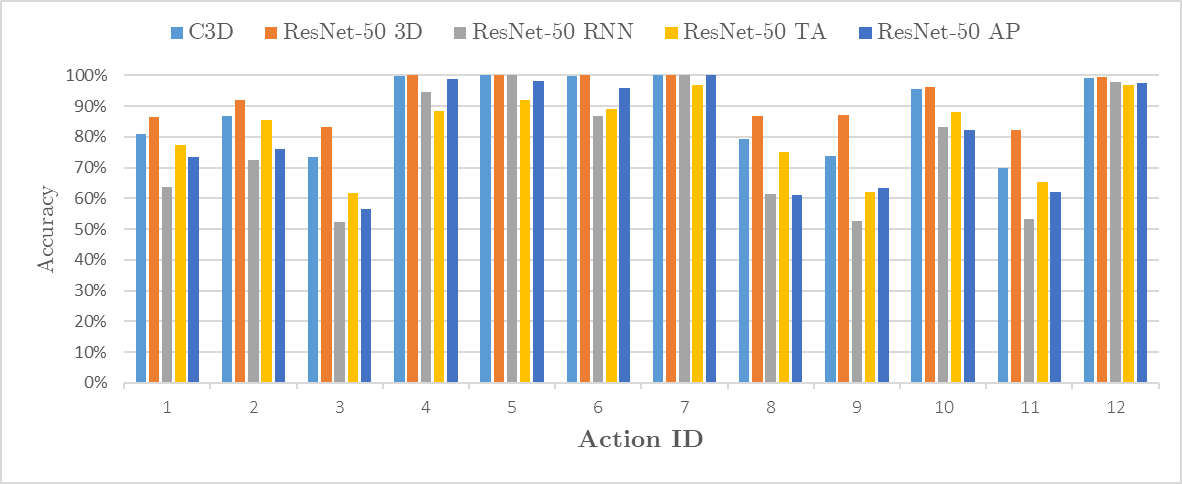
\includegraphics[width=0.8\linewidth]{figs/pc-MvDA_confusion_ixmas.png}
        \caption{Comparison of accuracy on each action class using different deep features combined with pc-MvDA on IXMAS dataset.}
        %\vspace{-0.3cm}
        \label{fig:pc-MvDA_confusion_ixmas}
    \end{figure}

    Table \ref{tab:sota_ixmas} compares the best combination of ResNet-50 3D and pc-MvDA with state-of-the-art frameworks. The comparison is for reference only because in other works, low-level hand-crafted video representation is used as private features and train-test strategy is leave-one-class out, which is not applicable to supervised deep feature extractors in this work. However, the results are still commensurable. % in circumstances where supervised approaches are adopted.
    % TODO - High priority

    \begin{table}[htbp]
    \centering
    \caption{Comparison of proposed methods with SOTA methods on IXMAS dataset according to the second evaluation protocol.}
    \resizebox{0.7\textwidth}{!}{
    \begin{tabular}{|c|c|c|}
    \hline
    Methods                                                              & Cross-view & Multi-view \\ \hline
    Liu et al. \cite{liu2011cross}                                   & 76.32      & N/A       \\ \hline
    Zheng et al. \cite{zheng2012cross}                               & 95.1       & 99.32     \\ \hline
    Zheng et al. \cite{zheng2016cross}                               & 97.8       & 99.4      \\ \hline
    Kong et al. \cite{kong2017deeply}                                & 99.92      & 100       \\ \hline
    Ulhaq et al. \cite{ulhaq2017space}                               & 66.82      & 92.47     \\ \hline
    Zhang et al. \cite{zhang2018cross}                               & 84.1       & N/A        \\ \hline
    Liu et al. \cite{liu2018learning}                                & N/A        & 90.3     \\ \hline
    Liu et al. \cite{liu2018hierarchically}                          & 99.95      & 99.67     \\ \hline
    Proposed method (ResNet-50 3D + pc-MvDA)                     & 99.67      & 99.65       \\ \hline
    \end{tabular}}
    \label{tab:sota_ixmas}
    \end{table}

    %!TEX root = ../../../main.tex

\subsection{Experimental results on MuHAVi dataset}
    \paragraph{1) Cross-view validation:} Table.\ref{tab:muhavi_cross} illustrates cross-view recognition results. The proposed pc-MvDA consistently produces a better average accuracy of around 96.19\% for protocol 1, approximately 4.55\% and 1.51\% higher than that of MvDA (91.64\%) and MvDA-vc (94.67\%) respectively.

    \begin{table}[htbp]
    \centering
    \caption{Cross-view recognition comparison on MuHAVi dataset.}
    \resizebox{0.8\textwidth}{!}{
    \begin{tabular}{|c|c|c|c|c|c|c|}
        \hline
        \multirow{2}{*}{Deep features}          & \multicolumn{3}{c|}{Protocol 1}   & \multicolumn{3}{c|}{Protocol 2}           \\ \cline{2-7} 
                                                & MvDA  & MvDA-vc & pc-MvDA         & MvDA  & MvDA-vc        & pc-MvDA          \\ \hline
        \multicolumn{1}{|c|}{C3D}               & 92.85 & 95.15   & \textbf{97.65}  & 98.95 & 99.76          & \textbf{100}     \\ \hline
        \multicolumn{1}{|c|}{ResNet-50 3D}      & 97.94 & 99.15   & \textbf{99.18}  & 96.77 & \textbf{99.94} & \textbf{99.94}   \\ \hline
        \multicolumn{1}{|c|}{ResNet-50 RNN}     & 95.54 & 95.14   & \textbf{96.18}  & 98.70 & 99.05          & \textbf{99.99}   \\ \hline
        \multicolumn{1}{|c|}{ResNet-50 TA}      & 85.80 & 88.95   & \textbf{91.12}  & 96.57 & 97.03          & \textbf{99.88}   \\ \hline
        \multicolumn{1}{|c|}{ResNet-50 AP}      & 86.09 & 94.98   & \textbf{96.82}  & 89.04 & 98.62          & \textbf{99.93}   \\ \hline
    \end{tabular}}
    \label{tab:muhavi_cross}
    \end{table}

    %Results in Table.\ref{tab:cross_feature_muhavi} show that our combination with ResNet-50 3D has the highest accuracies in almost every circumstances, even though both features coupled with our proposed pc-MvDA give satisfactory performance with all scores exceeding 91\%.

    \begin{table}[htbp]
    \centering
    \caption{Cross-view recognition results of different features on MuHAVi dataset with pc-MvDA method. The result in the bracket are accuracies of using features C3D, ResNet-50 3D, ResNet-50 RNN, ResNet-50 TA, ResNet-50 AP respectively. Each row corresponds to training view (from view C1 to view C7). Each column corresponds to testing view (from view C1 to view C7).}
    \resizebox{\textwidth}{!}{\begin{tabular}{|c|c|c|c|c|c|c|c|}
        \hline
        \backslashbox{Training}{Testing} & C1 & C2 & C3 & C4 & C5 & C6 & C7 \\ \hline
        C1 & N/A & \begin{tabular}{@{}c@{}} (96.1, \textbf{100}, 96.8, \\ 88.5, 98.5) \end{tabular} & \begin{tabular}{@{}c@{}} (98.6, \textbf{99.6}, 96.6, \\ 88.9, 96.3) \end{tabular} & \begin{tabular}{@{}c@{}} (98.6, \textbf{99.6}, 98.0, \\ 93.1, 98.2) \end{tabular} & \begin{tabular}{@{}c@{}} (97.7, \textbf{99.6}, 95.4, \\ 91.3, 96.1) \end{tabular} & \begin{tabular}{@{}c@{}} (97.7, \textbf{98.4}, 92.3, \\ 93.1, 96.3) \end{tabular} & \begin{tabular}{@{}c@{}} (98.2, \textbf{98.5}, 97.2, \\ 89.8, 97.1) \end{tabular} \\ \hline
        C2 & \begin{tabular}{@{}c@{}} (95.6, \textbf{99.0}, 95.2, \\ 91.3, 95.5) \end{tabular} & N/A & \begin{tabular}{@{}c@{}} (98.9, \textbf{99.6}, 96.9, \\ 90.3, 96.1) \end{tabular} & \begin{tabular}{@{}c@{}} (98.4, \textbf{99.6}, 97.6, \\ 92.6, 98.2) \end{tabular} & \begin{tabular}{@{}c@{}} (97.7, \textbf{99.6}, 95.4, \\ 90.9, 96.1) \end{tabular} & \begin{tabular}{@{}c@{}} (97.8, \textbf{98.4}, 92.7, \\ 93.6, 96.5) \end{tabular} & \begin{tabular}{@{}c@{}} (98.6, \textbf{99.0}, 97.4, \\ 90.6, 96.9) \end{tabular} \\ \hline
        C3 & \begin{tabular}{@{}c@{}} (96.1, \textbf{99.0}, 95.6, \\ 90.3, 95.1) \end{tabular} & \begin{tabular}{@{}c@{}} (97.0, \textbf{100}, 96.7, \\ 88.4, 97.8) \end{tabular} & N/A & \begin{tabular}{@{}c@{}} (98.1, \textbf{99.2}, 98.2, \\ 92.8, 98.2) \end{tabular} & \begin{tabular}{@{}c@{}} (97.9, \textbf{99.6}, 95.4, \\ 90.2, 95.6) \end{tabular} & \begin{tabular}{@{}c@{}} (97.9, \textbf{98.2}, 93.0, \\ 94.2, 96.5) \end{tabular} & \begin{tabular}{@{}c@{}} (97.8, \textbf{98.7}, 97.4, \\ 89.4, 97.6) \end{tabular} \\ \hline
        C4 & \begin{tabular}{@{}c@{}} (96.4, \textbf{98.8}, 95.4, \\ 89.6, 95.3) \end{tabular} & \begin{tabular}{@{}c@{}} (96.3, \textbf{100}, 96.6, \\ 91.0, 98.5) \end{tabular} & \begin{tabular}{@{}c@{}} (98.6, \textbf{99.6}, 97.3, \\ 89.5, 96.1) \end{tabular} & N/A & \begin{tabular}{@{}c@{}} (97.7, \textbf{99.4}, 95.6, \\ 91.3, 96.1) \end{tabular} & \begin{tabular}{@{}c@{}} (\textbf{98.4}, 98.0, 93.2, \\ 93.8, 95.6) \end{tabular} & \begin{tabular}{@{}c@{}} (97.7, \textbf{98.7}, 97.4, \\ 91.3, 96.7) \end{tabular} \\ \hline
        C5 & \begin{tabular}{@{}c@{}} (95.9, \textbf{99.0}, 95.6, \\ 91.3, 95.5) \end{tabular} & \begin{tabular}{@{}c@{}} (96.6, \textbf{100}, 97.1, \\ 89.9, 98.3) \end{tabular} & \begin{tabular}{@{}c@{}} (98.8, \textbf{99.4}, 96.8, \\ 90.7, 96.1) \end{tabular} & \begin{tabular}{@{}c@{}} (98.4, \textbf{99.6}, 98.0, \\ 92.1, 97.6) \end{tabular} & N/A & \begin{tabular}{@{}c@{}} (97.9, \textbf{98.2}, 93.4, \\ 94.4, 96.8) \end{tabular} & \begin{tabular}{@{}c@{}} (98.0, \textbf{98.7}, 96.9, \\ 89.0, 97.8) \end{tabular} \\ \hline
        C6 & \begin{tabular}{@{}c@{}} (95.8, \textbf{99.0}, 95.8, \\ 90.3, 95.0) \end{tabular} & \begin{tabular}{@{}c@{}} (97.0, \textbf{100}, 97.6, \\ 89.7, 98.5) \end{tabular} & \begin{tabular}{@{}c@{}} (98.8, \textbf{99.6}, 96.9, \\ 88.7, 96.1) \end{tabular} & \begin{tabular}{@{}c@{}} (98.4, \textbf{99.4}, 98.0, \\ 92.8, 98.2) \end{tabular} & \begin{tabular}{@{}c@{}} (97.5, \textbf{99.6}, 95.9, \\ 91.2, 95.5) \end{tabular} & N/A & \begin{tabular}{@{}c@{}} (98.2, \textbf{99.0}, 97.2, \\ 90.7, 97.4) \end{tabular} \\ \hline
        C7 & \begin{tabular}{@{}c@{}} (96.2, \textbf{98.8}, 95.7, \\ 91.5, 96.2) \end{tabular} & \begin{tabular}{@{}c@{}} (96.4, \textbf{100}, 97.5, \\ 90.3, 98.5) \end{tabular} & \begin{tabular}{@{}c@{}} (98.4, \textbf{99.0}, 97.3, \\ 90.0, 96.7) \end{tabular} & \begin{tabular}{@{}c@{}} (\textbf{98.8}, 98.8, 98.2, \\ 92.8, 98.0) \end{tabular} & \begin{tabular}{@{}c@{}} (97.5, \textbf{99.8}, 95.9, \\ 91.5, 95.9) \end{tabular} & \begin{tabular}{@{}c@{}} (\textbf{98.9}, 98.2, 92.8, \\ 93.9, 97.1) \end{tabular} & N/A \\ \hline
    \end{tabular}}
    \label{tab:cross_feature_muhavi}
    \end{table}

    \paragraph{2) Multi-view validation}: Table.\ref{tab:muhavi_multi} shows multi-view recognition results. The first protocol shows very close capability of MvDA-vc and pc-MvDA at 95.54\% and 95.83\% whereas MvDA is about 3\% behind at 92.7\%. For the second protocol, our variant exceeds MvDA by 2.21\% and MvDA-vc by 1.49\%. The near perfect results of the second protocol give us the same indication that it is not an inequitable method of comparison of MvA algorithms. 

    \begin{table}[htbp]
    \centering
    \caption{Multi-view recognition comparison on MuHAVi dataset.}
    \resizebox{0.8\textwidth}{!}{
    \begin{tabular}{|c|c|c|c|c|c|c|}
        \hline
        \multirow{2}{*}{Deep features}          & \multicolumn{3}{c|}{Protocol 1}                   & \multicolumn{3}{c|}{Protocol2}            \\ \cline{2-7} 
                                                & MvDA           & MvDA-vc        & pc-MvDA         & MvDA           & MvDA-vc & pc-MvDA        \\ \hline
        \multicolumn{1}{|c|}{C3D}               & 81.80          & 96.05          & \textbf{97.37}  & 88.39          & 99.61   & \textbf{100}   \\ \hline
        \multicolumn{1}{|c|}{ResNet-50 3D}      & 99.07          & 99.12          & \textbf{99.15}  & \textbf{99.98} & 99.96   & 99.89          \\ \hline
        \multicolumn{1}{|c|}{ResNet-50 RNN}     & \textbf{96.18} & 95.55          & 95.97           & \textbf{100}   & 99.00   & 99.98          \\ \hline
        \multicolumn{1}{|c|}{ResNet-50 TA}      & \textbf{90.45} & 89.73          & 90.22           & \textbf{99.92} & 98.17   & 99.72          \\ \hline
        \multicolumn{1}{|c|}{ResNet-50 AP}      & 96.01          & \textbf{96.75} & 96.42           & \textbf{100}   & 95.13   & 99.68          \\ \hline
    \end{tabular}}
    \label{tab:muhavi_multi}
    \end{table}

    Figure \ref{fig:pc-MvDA_confusion_muhavi} compares the performance of feature extractors regarding each action class in multi-view evaluation scheme combined with protocol 1. For this dataset, ResNet-50 3D persistently yields out-standing performance while ResNet-50 TA has the worst recognition rates in all action classes.

    \begin{figure}[htbp]
        \centering
        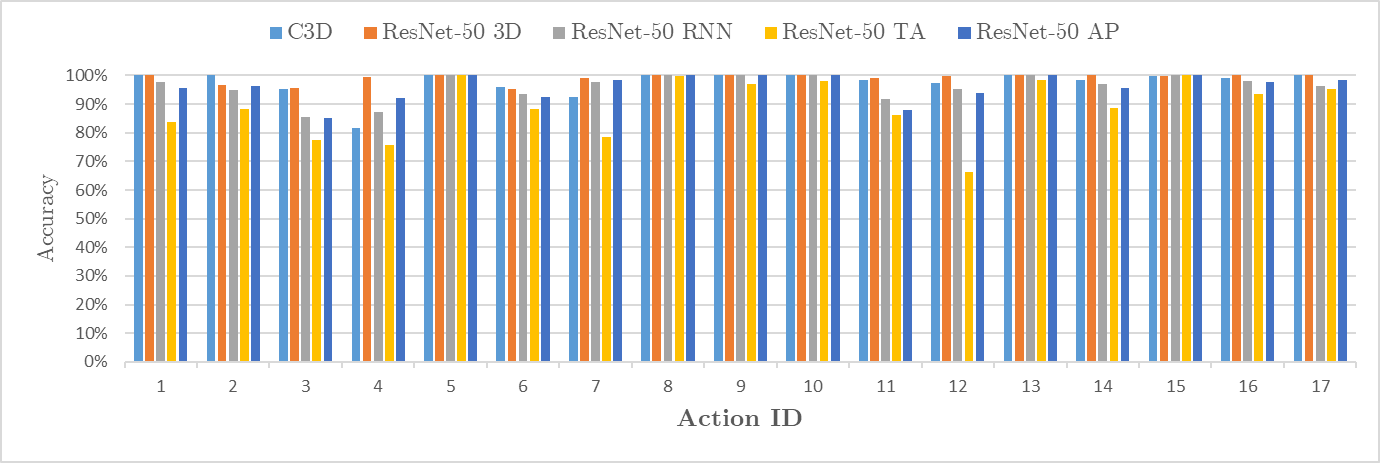
\includegraphics[width=1.0\linewidth]{figs/pc-MvDA_confusion_muhavi.png}
        \caption{Comparison of accuracy on each action class using different deep features combined with pc-MvDA.}
        %\vspace{-0.3cm}
        \label{fig:pc-MvDA_confusion_muhavi}
    \end{figure}

    Table \ref{tab:sota_muhavi} compares the best investigated combination of ResNet-50 3D and pc-MvDA with state-of-the-art frameworks. The comparison is for reference only because of aforementioned difference in setup of number of views and cross validation scheme.

    \begin{table}[htbp]
    \centering
    \caption{Comparison of the proposed methods with SOTA methods on MuHAVi dataset according to the second evaluation protocol.}
    \resizebox{0.7\textwidth}{!}{
    \begin{tabular}{|c|c|c|}
    \hline
    Methods                                                   & Cross-view & Multi-view \\ \hline
    Wu et al. \cite{wu2012view}                               & N/A       & 94.5     \\ \hline
    Zheng et al. \cite{zheng2016cross}                        & 94.88     & 99.8     \\ \hline
    Liu et al. \cite{liu2018learning}                         & N/A       & 91.2     \\ \hline
    Liu et al. \cite{liu2018hierarchically}                   & 99.91     & 99.8     \\ \hline
    Proposed method (ResNet-50 3D + pc-MvDA) \protect\footnotemark              & 99.90     & 99.88    \\ \hline
    \end{tabular}}
    \label{tab:sota_muhavi}
    \end{table}
    \footnotetext{Results when choosing only 4 views Camera 1, Camera 3, Camera 4 and Camera 6 following the other works.}

    %!TEX root = ../../../main.tex

\subsection{Experimental results on MICAGes dataset}

    \paragraph{1) Cross-view validation:} It can be seen in Table.\ref{tab:mica_cross} that pc-MvDA outperforms in almost every cases. With the first protocol, the norm accuracy of pc-MvDA of 74.52\% surpasses that of MvDA-vc (72.12\%) by 2.4\% and that of MvDA (64.94\%) by a large margin of 9.58\%. Especially in case of C3D features, the proposed algorithm achieved 90.2\% recognition rate whereas MvDA returns only 67.13\%.

    \begin{table}[htbp]
    \centering
    \caption{Cross-view recognition comparison on MICAGes dataset.}
    \resizebox{0.8\textwidth}{!}{
    \begin{tabular}{|c|c|c|c|c|c|c|}
        \hline
        \multirow{2}{*}{Deep features}          & \multicolumn{3}{c|}{Protocol 1}          & \multicolumn{3}{c|}{Protocol 2}            \\ \cline{2-7} 
                                                & MvDA  & MvDA-vc        & pc-MvDA         & MvDA  & MvDA-vc        & pc-MvDA           \\ \hline
        \multicolumn{1}{|c|}{C3D}               & 67.13 & 85.98          & \textbf{90.20}  & 93.74 & 99.80          & \textbf{100}      \\ \hline
        \multicolumn{1}{|c|}{ResNet-50 3D}      & 94.91 & 95.25          & \textbf{95.62}  & 97.43 & \textbf{99.97} & 99.79             \\ \hline
        \multicolumn{1}{|c|}{ResNet-50 RNN}     & 58.01 & 61.64          & \textbf{64.13}  & 100   & 100            & 100               \\ \hline
        \multicolumn{1}{|c|}{ResNet-50 TA}      & 53.58 & \textbf{59.55} & 58.62           & 96.70 & 99.48          & \textbf{99.83}    \\ \hline
        \multicolumn{1}{|c|}{ResNet-50 AP}      & 51.07 & 58.19          & \textbf{64.04}  & 99.73 & \textbf{99.99} & 99.89             \\ \hline
    \end{tabular}}
    \label{tab:mica_cross}
    \end{table}

    %Table.\ref{tab:cross_feature_mica} compares all types of deep features regarding accuracy of the proposed algorithm. 
    The top ranking of features applies identically and radically proves the superiority of 3D convolution based clip-level feature extraction in video recognition: ResNet-50 3D at 95.62\% and C3D at 90.2\%. The rest are ResNet-50 RNN (64.13\%), ResNet-50 AP (64.04\%) and ResNet-50 TA (58.62\%). For the second protocol, MvDA-vc (99.85\%) and pc-MvDA (99.9\%) are nearly even in performance while MvDA achieved 97.52\%.

    \begin{table}[htbp]
    \centering
    \caption{Cross-view recognition results of different features on MICAGes dataset with pc-MvDA method. The result in the bracket are accuracies of using features C3D, ResNet-50 3D, ResNet-50 RNN, ResNet-50 TA, RestNet-50 AP respectively. Each row corresponds to training view (from view K1 to view K5). Each column corresponds to testing view (from view K1 to view K5).}
    \resizebox{\textwidth}{!}{\begin{tabular}{|c|c|c|c|c|c|}
        \hline
        \backslashbox{Training}{Testing} & K1 & K2 & K3 & K4 & K5 \\ \hline
        K1 & N/A & \begin{tabular}{@{}c@{}} (92.9, \textbf{95.5}, 69.4, \\ 63.9, 65.1) \end{tabular} & \begin{tabular}{@{}c@{}} (93.7, \textbf{98.0}, 79.1, \\ 75.8, 74.7) \end{tabular} & \begin{tabular}{@{}c@{}} (90.5, \textbf{97.6}, 64.5, \\ 68.8, 70.8) \end{tabular} & \begin{tabular}{@{}c@{}} (89.2, \textbf{92.6}, 56.0, \\ 43.7, 58.2) \end{tabular} \\ \hline       
        K2 & \begin{tabular}{@{}c@{}} (84.7, \textbf{94.6}, 51.3, \\ 41.4, 53.7) \end{tabular} & N/A & \begin{tabular}{@{}c@{}} (94.6, \textbf{97.6}, 78.9, \\ 75.4, 77.5) \end{tabular} & \begin{tabular}{@{}c@{}} (91.3, \textbf{97.6}, 64.4, \\ 68.5, 68.0) \end{tabular} & \begin{tabular}{@{}c@{}} (87.4, \textbf{92.7}, 56.1, \\ 42.0, 55.6) \end{tabular} \\ \hline       
        K3 & \begin{tabular}{@{}c@{}} (87.5, \textbf{94.9}, 51.9, \\ 43.6, 52.7) \end{tabular} & \begin{tabular}{@{}c@{}} (93.0, \textbf{95.5}, 70.1, \\ 64.7, 63.4) \end{tabular} & N/A & \begin{tabular}{@{}c@{}} (90.0, \textbf{97.6}, 63.2, \\ 62.6, 67.5) \end{tabular} & \begin{tabular}{@{}c@{}} (88.9, \textbf{92.2}, 57.2, \\ 41.8, 56.6) \end{tabular} \\ \hline       
        K4 & \begin{tabular}{@{}c@{}} (86.7, \textbf{94.7}, 50.8, \\ 48.9, 54.9) \end{tabular} & \begin{tabular}{@{}c@{}} (90.2, \textbf{95.5}, 71.5, \\ 68.2, 61.8) \end{tabular} & \begin{tabular}{@{}c@{}} (92.5, \textbf{98.0}, 81.0, \\ 76.0, 74.4) \end{tabular} & N/A & \begin{tabular}{@{}c@{}} (89.7, \textbf{92.3}, 54.3, \\ 44.9, 56.6) \end{tabular} \\ \hline       
        K5 & \begin{tabular}{@{}c@{}} (84.9, \textbf{94.9}, 48.4, \\ 41.5, 57.9) \end{tabular} & \begin{tabular}{@{}c@{}} (90.4, \textbf{95.5}, 72.6, \\ 64.1, 65.7) \end{tabular} & \begin{tabular}{@{}c@{}} (94.0, \textbf{97.8}, 79.1, \\ 72.5, 76.3) \end{tabular} & \begin{tabular}{@{}c@{}} (91.9, \textbf{97.3}, 62.7, \\ 64.1, 69.0) \end{tabular} & N/A \\ \hline
    \end{tabular}}
    \label{tab:cross_feature_mica}
    \end{table}

    \paragraph{2) Multi-view validation}: The multi-view recognition results in Table.\ref{tab:mica_multi} shows an almost alike trend for both protocols. In general, pc-MvDA is 8.95\% and 0.72\% higher in accuracy for protocol 1, and 2.75\% and 0.04\% for protocol 2, in comparison with MvDA and MvDA-pc respectively.

    % TODO
    In virtually every experiments of MICAGes and two earlier benchmark datasets, the proposed extension is superior. The average accuracies of pc-MvDA is, in comparison on protocol 1 (and protocol 2 resp.), 5.29\% (1.21\% resp.) higher than MvDA, 1.21\% (0.62\% resp.) better than MvDA-vc. Despite not being as intuitive and straightly intelligible as pairwise-covariance, the multi-view resemblance added in MvDA-vc achieved nearly the performance of pc-MvDA. However, this view-consistency can be easily splitted into pairwise terms and intergrated into the objective of pc-MvDA in future works for further analysis.

    \begin{table}[htbp]
    \centering
    \caption{Multi-view recognition comparison on MICAGes dataset.}
    \resizebox{0.8\textwidth}{!}{
    \begin{tabular}{|c|c|c|c|c|c|c|}
        \hline
        \multirow{2}{*}{Deep features}          & \multicolumn{3}{c|}{Protocol 1}          & \multicolumn{3}{c|}{Protocol2}                     \\ \cline{2-7} 
                                                & MvDA  & MvDA-vc        & pc-MvDA         & MvDA           & MvDA-vc       & pc-MvDA           \\ \hline
        \multicolumn{1}{|c|}{C3D}               & 68.31 & 87.70          & \textbf{89.99}  & 88.79          & 99.54         & \textbf{100}      \\ \hline
        \multicolumn{1}{|c|}{ResNet-50 3D}      & 95.32 & 95.26          & \textbf{95.54}  & \textbf{100}   & 99.96         & 99.80             \\ \hline
        \multicolumn{1}{|c|}{ResNet-50 RNN}     & 57.50 & 63.05          & \textbf{63.83}  & 99.90          & \textbf{100}  & 99.97             \\ \hline
        \multicolumn{1}{|c|}{ResNet-50 TA}      & 54.43 & \textbf{61.46} & 58.25           & 96.72          & 99.49         & \textbf{99.69}    \\ \hline
        \multicolumn{1}{|c|}{ResNet-50 AP}      & 50.93 & 60.20          & \textbf{63.66}  & \textbf{99.99} & 99.93         & 99.67             \\ \hline
    \end{tabular}}
    \label{tab:mica_multi}
    \end{table}

    In addition to the same propensity shown, MICAGes also reveals the robustness of 3D convolution to generate fine clustered private feature space because this dataset contains exclusively hand gestures, which take part in a relatively small region of the captured videos. ResNet-50 3D and C3D are predominant for discriminant common space construction and classification and distances other features (Figure \ref{fig:pc-MvDA_confusion_mica}).

    \begin{figure}[htbp]
        \centering
        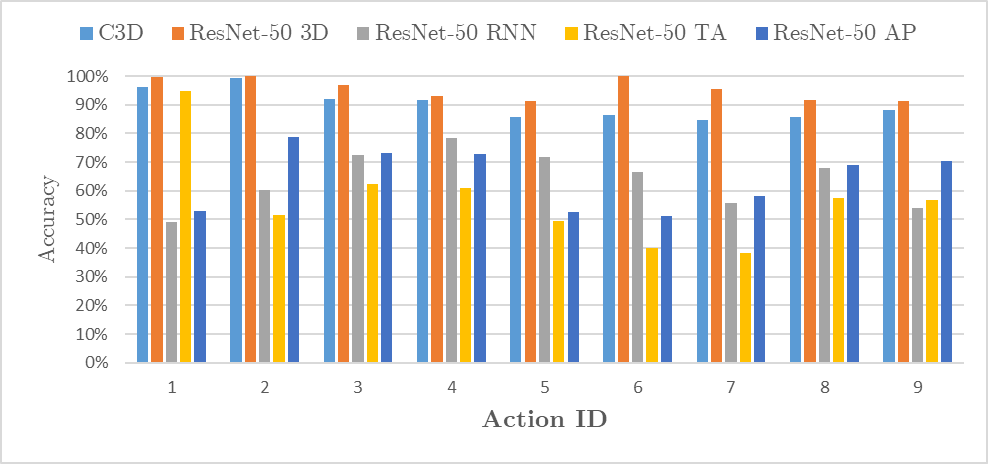
\includegraphics[width=0.8\linewidth]{figs/pc-MvDA_confusion_mica.png}
        \caption{Comparison of accuracy on each action class using different deep features combined with pc-MvDA on MICAGes dataset.}
        %\vspace{-0.3cm}
        \label{fig:pc-MvDA_confusion_mica}
    \end{figure}

    To better study the behavior of investigated multi-view analysis algorithms, t-SNE embedding of original private spaces, MvDA and pc-MvDA common space generated by protocol 1 are plotted in Figure \ref{fig:mica-tsne}. In these scatter plots, colors denote action classes, shapes as different views and train/test data are distinguished by border type. They explicitly denotes the surpassing capability of the proposed algorithm in finding a common space with prominent extra-class discrepancy. The data samples involved in training process are generally clustered in compact and separated blobs while testing data samples dissolve nearby. The better convergence of pc-MvDA compared to the baseline is usually only visible for harder features, whereas with the inputs of ResNet-50 3D features, which are already highly discriminated in private spaces, the improvement of pc-MvDA is negligible. Note that these illustrations of t-SNE embedding do not strictly depict an identical distribution of data.

    \begin{figure}[htbp]
        \centering
        \includegraphics[width=1\linewidth, height=0.6\pdfpageheight, keepaspectratio=false]{figs/mica-tsne.png}
        \caption{First column: private feature spaces stacked and embedded together in a same coordinate system; Second column: MvDA common space; Third column: pc-MvDA common space.}
        %\vspace{-0.3cm}
        \label{fig:mica-tsne}
    \end{figure}


    %!TEX root = ../main.tex

\cleardoublepage
\ihead[]{Appendix}
\ohead[]{\pagemark}
\begin{appendix}
\chapter{Appendix} \label{chap:appendix}

\section{Derivation} \label{app:derivation}

This chapter supplies the expansion formulas of equations regarding multi-view analysis algorithms mentioned in this thesis, including MvDA, MvDA-vc and the proposed pc-MvDA.

For easy follow-up, let us briefly reduplicate the definitions and notations that will be used.
$X = \left[X_1, X_2, ..., X_v\right] = \{x_{ijk}|i=(1,..,c);j = (1,..,v);k=(1,..,n_{ij})\}$ and $Y = \left[Y_1, Y_2, ..., Y_v\right] = \{y_{ijk} = w_j^T x_{ijk}|i=(1,..,c); j=(1,..,v); k=(1,...,n_{ij})\}$ stand for the $v$-view dataset of $c$ classes and $n$ samples before and after projection respectively.
The mean of dataset is designated with $\mu = \frac{1}{n}\sum_{i=1}^{c}\sum_{j=1}^{v}\sum_{k=1}^{n_{ij}}y_{ijk}$, mean of class $\mu_{i} = \frac{1}{n_i}\sum_{j=1}^{v}\sum_{k=1}^{n_{ij}}y_{ijk}$ and mean of class in one view $\mu_{ij} = \frac{1}{n_{ij}}\sum_{k=1}^{n_{ij}}y_{ijk}$.
$W = \left[\omega_1, \omega_2, ..., \omega_v\right]$ are $v$ transformations learnt for each view by solving an optimization problem that minimizes within-class scatter matrix $\boldsymbol{S}^y_W$ and maximizes between-class scatter matrix $\boldsymbol{S}^y_B$.
Here the ubiquitous subscripts $i, a, b$ denote class, $j, r$ denote view and $k$ denotes index; while the less-frequently used superscripts $x$ and $y$ allude the original or transformed common dimension respectively of the corresponding term.

Supposing data samples from all views are aligned identically, in essence, the $k^{th}$ sample of $X_j$ is the common component of $k^{th}$ sample of $X_r$ $\forall j, r \in (1, 2, ..., v)$.
In addition to the aformentioned notations, we define the class vector $e_i \in \mathbb{R}^{\frac{n}{v}\times 1}$ of class $i$, which has $k^{th}$ element ${e_i}_{(k)} = 1$ if $class(x_k) = i$ and ${e_i}_{(k)} = 0$ otherwise.
It follows that $e = \sum_{i=1}^{c}e_i$ is a vector of ones as each sample strictly belongs to one class.

By using class vector $e_i$ as mask over $X_j$, mean of class $i$ in original dimension of view $j$ can be expressed by:
\begin{equation}
    \mu^{(x)}_{ij} = \frac{1}{n_{ij}}\sum_{k=1}^{n_{ij}}x_{ijk} = \frac{1}{n_{ij}}X_j e_i
    \label{eq:mean_from_class_vector}
\end{equation}

\subsection{Derivation of \texorpdfstring{$\boldsymbol{S}^y_W$}{intra-class} and \texorpdfstring{$\boldsymbol{S}^y_B$}{inter-class} scatter matrices in MvDA} \label{subsec:derivation_mvda}
    The expansions of $\boldsymbol{S}^y_W$ and $\boldsymbol{S}^y_B$ used in this thesis slightly differ from those supplemented in the original publication \cite{kan2015multi} in order to derive the pre-transformed version $\boldsymbol{S}^x_W$ and $\boldsymbol{S}^x_B$ and thus requires extra reformulation from the steps where we can subtitute \eqref{eq:mean_from_class_vector} in.

    The within-class scatter matrix $\boldsymbol{S}^y_W$ of MvDA in Equation \eqref{eq:MvDA_Sw} is expanded as follows:
    \begin{equation}
        \begin{split}
            \boldsymbol{S}^y_W &= \sum_{i=1}^{c}\sum_{j=1}^{v}\sum_{k=1}^{n_{ij}}(y_{ijk}-\mu_i)(y_{ijk}-\mu_i)^T \\
            &= \sum_{i=1}^{c}\sum_{j=1}^{v}\sum_{k=1}^{n_{ij}}\left(y_{ijk}y_{ijk}^T - y_{ijk}\mu_i^T - \mu_iy_{ijk}^T + \mu_i\mu_i^T\right) \\
            &= \sum_{i=1}^{c}\left(\sum_{j=1}^{v}\sum_{k=1}^{n_{ij}}y_{ijk}y_{ijk}^T - n_i\mu_i\mu_i^T\right) \\
            &= \sum_{i=1}^{c}\left(\sum_{j=1}^{v}\sum_{k=1}^{n_{ij}}y_{ijk}y_{ijk}^T - \frac{1}{n_i}\left(\sum_{j=1}^{v}n_{ij}\mu_{ij}\right){\left(\sum_{j=1}^{v}n_{ij}\mu_{ij}\right)}^T\right) \\
            &= \sum_{i=1}^{c}\left(\sum_{j=1}^{v}\sum_{k=1}^{n_{ij}}y_{ijk}y_{ijk}^T - \frac{1}{n_i}\sum_{j=1}^{v}\sum_{r=1}^{v}n_{ij}n_{ir}\mu_{ij}\mu_{ir}^T\right) \\
            &= \sum_{j=1}^{v}\omega_j^T\left(\sum_{i=1}^{c}\sum_{k=1}^{n_{ij}}x_{ijk}x_{ijk}^T\right)\omega_j - \sum_{j=1}^{v}\sum_{r=1}^{v}\omega_j^T\left(\sum_{i=1}^{c}\frac{n_{ij}n_{ir}}{n_i}\mu^{(x)}_{ij}{\mu^{(x)}_{ir}}^T\right)\omega_r \\
            &= \sum_{j=1}^{v}\omega_j^T X_j I X_j^T\omega_j - \sum_{j=1}^{v}\sum_{r=1}^{v}\omega_j^T\left(\sum_{i=1}^{c}\frac{n_{ij}n_{ir}}{n_i}\left(\frac{1}{n_{ij}}X_j e_i\right)\left(\frac{1}{n_{ir}}X_r e_i\right)^T\right)\omega_r \\
            &= \sum_{j=1}^{v}\omega_j^T X_j I X_j^T\omega_j - \sum_{j=1}^{v}\sum_{r=1}^{v}\omega_j^T\left(\sum_{i=1}^{c}\frac{1}{n_i}X_j e_i e_i^T X_r^T\right)\omega_r \\
            &= \sum_{j=1}^{v}\omega_j^T X_j I X_j^T\omega_j - \sum_{j=1}^{v}\sum_{r=1}^{v}\omega_j^T X_j\left(\sum_{i=1}^{c}\frac{1}{n_i}e_i e_i^T\right)X_r^T\omega_r \\
            &= \sum_{j=1}^{v}\omega_j^T X_j I X_j^T\omega_j - \sum_{j=1}^{v}\sum_{r=1}^{v}\omega_j^T X_j E X_r^T\omega_r \\
            &= W^T X \boldsymbol{I} X^T W - W^T X \boldsymbol{E} X^T W \\
            &= W^T X \left(\boldsymbol{I} - \boldsymbol{E}\right) X^T W \\
            \Rightarrow \boldsymbol{S}^x_W &= X \left(\boldsymbol{I} - \boldsymbol{E}\right) X^T
        \end{split}
        \label{eq:mvda_Sw_derivation}
    \end{equation}
    where $I \in \mathbb{R}^{\frac{n}{v}\times \frac{n}{v}}$ and $\boldsymbol{I} \in \mathbb{R}^{n\times n}$ are identity matrices; $E = \sum_{i=1}^{c}\frac{1}{n_i}e_i e_i^T \in \mathbb{R}^{\frac{n}{v}\times \frac{n}{v}}$ is a square matrix whose elements satisfy:
    \begin{equation}
        \boldsymbol{E}_{(k,l)} = \left\{\begin{array}{lr}
            \frac{1}{n_i}, & \text{if } class(x_k) = class(x_l) = i\\
            0, & \text{otherwise}
            \end{array}\right\}
    \end{equation}
    and $\boldsymbol{E} = \left[E\right]_{v\times v} \in \mathbb{R}^{n\times n}$ is $v \times v$ grid stack of $E$:
    \begin{equation}
        \boldsymbol{E} = \left[\begin{matrix}E&E&\cdots&E\\E&E&\cdots&E\\\vdots&\vdots&\ddots&\vdots\\E&E&\cdots&E\\\end{matrix}\right]
    \end{equation}

    Using the distributivity identity of summation, it is easy to prove that:
    \begin{equation}
        \sum_{a=1}^{c}\sum_{b=1}^{c}e_a e_b^T = \left(\sum_{i=1}^{c}e_i\right)\left(\sum_{i=1}^{c}e_i^T\right) = ee^T
    \end{equation}
    where $e$ is a vector of ones, hence, its self product results in a square matrix of ones.
    Then, the between-class scatter matrix $\boldsymbol{S}^y_B$ of MvDA in Equation \eqref{eq:MvDA_Sb} can be expanded as follows:
    \begin{equation}
        \begin{split}
            \boldsymbol{S}^y_B &= \sum_{i=1}^{c}n_i\left(\mu_i - \mu\right)\left(\mu_i - \mu\right)^T \\
            &= \sum_{i=1}^{c}n_i\left(\mu_i\mu_i^T - \mu_i\mu^T - \mu\mu_i^T + \mu\mu^T\right) \\
            &= \sum_{i=1}^{c}n_i\mu_i\mu_i^T - n\mu\mu^T \\
            &= \sum_{i=1}^{c}n_i\left(\frac{1}{n_i}\sum_{j=1}^{v}n_{ij}\mu_{ij}\right)\left(\frac{1}{n_i}\sum_{j=1}^{v}n_{ij}\mu_{ij}\right)^T - n\left(\frac{1}{n}\sum_{i=1}^{c}\sum_{j=1}^{v}n_{ij}\mu_{ij}\right)\left(\frac{1}{n}\sum_{i=1}^{c}\sum_{j=1}^{v}n_{ij}\mu_{ij}\right)^T \\
            &= \sum_{i=1}^{c}\frac{1}{n_i}\left(\sum_{j=1}^{v}\sum_{r=1}^{v}n_{ij}n_{ir}\mu_{ij}\mu_{ir}^T\right) - \frac{1}{n}\left(\sum_{j=1}^{v}\sum_{i=1}^{c}n_{ij}\mu_{ij}\right)\left(\sum_{j=1}^{v}\sum_{i=1}^{c}n_{ij}\mu_{ij}\right)^T \\
            &= \sum_{j=1}^{v}\sum_{r=1}^{v}\left(\sum_{i=1}^{c}\frac{n_{ij}n_{ir}}{n_i}\mu_{ij}\mu_{ir}^T\right) - \frac{1}{n}\sum_{j=1}^{v}\sum_{r=1}^{v}\left(\sum_{i=1}^{c}n_{ij}\mu_{ij}\right)\left(\sum_{i=1}^{c}n_{ij}\mu_{ij}\right)^T \\
            &= \sum_{j=1}^{v}\sum_{r=1}^{v}\left(\sum_{i=1}^{c}\frac{n_{ij}n_{ir}}{n_i}\mu_{ij}\mu_{ir}^T\right) - \frac{1}{n}\sum_{j=1}^{v}\sum_{r=1}^{v}\left(\sum_{a=1}^{c}\sum_{b=1}^{c}n_{aj}n_{br}\mu_{aj}\mu_{br}^T\right) \\
            &= \sum_{j=1}^{v}\sum_{r=1}^{v}\omega_j^T\left(\sum_{i=1}^{c}\frac{n_{ij}n_{ir}}{n_i}\mu^{(x)}_{ij}{\mu^{(x)}_{ir}}^T\right)\omega_r - \sum_{j=1}^{v}\sum_{r=1}^{v}\omega_j^T\left(\sum_{a=1}^{c}\sum_{b=1}^{c}\frac{n_{aj}n_{br}}{n}\mu^{(x)}_{aj}{\mu^{(x)}_{br}}^T\right)\omega_r \\
            &= \sum_{j=1}^{v}\sum_{r=1}^{v}\omega_j^T\left(\sum_{i=1}^{c}\frac{n_{ij}n_{ir}}{n_i}\left(\frac{1}{n_{ij}}X_j e_i\right)\left(\frac{1}{n_{ir}}X_r e_i\right)^T\right)\omega_r \\
            &\ \ \ \ \ \ \ \ \ \ \ \ \ \ \ \ \ \ \ \ \ \ \ \ \ \ \ \ \ \  - \sum_{j=1}^{v}\sum_{r=1}^{v}\omega_j^T\left(\sum_{a=1}^{c}\sum_{b=1}^{c}\frac{n_{aj}n_{br}}{n}\left(\frac{1}{n_{aj}}X_j e_a\right)\left(\frac{1}{n_{br}}X_r e_b\right)\right)\omega_r \\
            &= \sum_{j=1}^{v}\sum_{r=1}^{v}\omega_j^T X_j\left(\sum_{i=1}^{c}\frac{1}{n_i}e_i e_i^T\right)X_r^T\omega_r - \sum_{j=1}^{v}\sum_{r=1}^{v}\omega_j^T X_j\left(\sum_{a=1}^{c}\sum_{b=1}^{c}\frac{1}{n}e_a e_b^T\right)X_r^T\omega_r \\
            &= \sum_{j=1}^{v}\sum_{r=1}^{v} \omega_j^T X_j E X_r^T \omega_r - \sum_{j=1}^{v}\sum_{r=1}^{v} \omega_j^T X_j \frac{1}{n}\mathbbm{1} X_r^T \omega_r \\
            &= W^T X \boldsymbol{E} X^T W - W^T X \frac{1}{n}\boldsymbol{\mathbbm{1}} X^T W \\
            &= W^T X \left(\boldsymbol{E} - \frac{1}{n}\boldsymbol{\mathbbm{1}}\right) X^T W \\
            \Rightarrow \boldsymbol{S}^x_B &= X \left(\boldsymbol{E} - \frac{1}{n}\boldsymbol{\mathbbm{1}}\right) X^T
        \end{split}
        \label{eq:mvda_Sb_derivation}
    \end{equation}
    where $E = \sum_{i=1}^{c}\frac{1}{n_i}e_i e_i^T \in \mathbb{R}^{\frac{n}{v}\times \frac{n}{v}}$ and $\boldsymbol{E} = \left[E\right]_{v\times v} \in \mathbb{R}^{n\times n}$ are defined above; $\mathbbm{1} = \sum_{a=1}^{c}\sum_{b=1}^{c}e_a e_b^T = \left[1\right]_{\frac{n}{v} \times \frac{n}{v}} \in \mathbb{R}^{\frac{n}{v}\times \frac{n}{v}}$ and $\boldsymbol{\mathbbm{1}} = \left[\mathbbm{1}\right]_{v\times v} = \left[1\right]_{n \times n} \in \mathbb{R}^{n\times n}$ are matrices of ones.

\subsection{Derivation of \texorpdfstring{$\boldsymbol{O}_{view-consistency}$}{view-consistency term} in MvDA-vc} \label{subsec:derivation_mvdavc}

    The view-consistency objective of MvDA-vc in Equation \eqref{eq:MvDA-vc_vc} is expanded as follows:
    \begin{equation}
        \begin{split}
            \boldsymbol{O}_{view-consistency} &= \sum_{j=1}^{v}\sum_{r=1}^{v}\left|\left|\boldsymbol{\beta}_j - \boldsymbol{\beta}_r\right|\right|_2^2 \\
            &= \sum_{j=1}^{v}\sum_{r=1}^{v}\left(\boldsymbol{\beta}_j^T\boldsymbol{\beta}_j - \boldsymbol{\beta}_j^T\boldsymbol{\beta}_r - \boldsymbol{\beta}_r^T\boldsymbol{\beta}_j + \boldsymbol{\beta}_r^T\boldsymbol{\beta}_r\right) \\
            &= \sum_{j=1}^{v}\sum_{r=1}^{v}\left(2\boldsymbol{\beta}_j^T\boldsymbol{\beta}_j - 2\boldsymbol{\beta}_j^T\boldsymbol{\beta}_r\right) \\
            &= \sum_{j=1}^{v}2v\omega_j^T\boldsymbol{P}_j I \boldsymbol{P}_j^T\omega_j - \sum_{j=1}^{v}\sum_{r=1}^{v}2\omega_j^T\boldsymbol{P}_j I \boldsymbol{P}_r^T\omega_r \\
            &= W^T \boldsymbol{P}^T \left(2v\boldsymbol{I}\right) \boldsymbol{P} W - W^T \boldsymbol{P}^T \left(2\boldsymbol{\widehat{I}}\right) \boldsymbol{P} W \\
            &= W^T \boldsymbol{P}^T \left(2v\boldsymbol{I} - 2\boldsymbol{\widehat{I}}\right) \boldsymbol{P} W
        \end{split}
        \label{eq:mvdavc_vc_derivation}
    \end{equation}
    where $\boldsymbol{\beta}_j = \boldsymbol{P}_j\omega_j$ and $\boldsymbol{P}_j = \left(X_j^T X_j\right)^{-1}X_j^T$ as defined in Section \ref{subsubsec:mvdavc}; $I \in \mathbb{R}^{\frac{n}{v}\times \frac{n}{v}}$ and $\boldsymbol{I} \in \mathbb{R}^{n\times n}$ are defined in \ref{subsec:derivation_mvda}, $\boldsymbol{\widehat{I}} = \left[I\right]_{v\times v} \in \mathbb{R}^{n\times n}$ is $v\times v$ grid stack of $I$:
    \begin{equation}
        \boldsymbol{\widehat{I}} = \left[\begin{matrix}I&I&\cdots&I\\I&I&\cdots&I\\\vdots&\vdots&\ddots&\vdots\\I&I&\cdots&I\\\end{matrix}\right]
    \end{equation}

\subsection{Derivation of \texorpdfstring{${\boldsymbol{S}^x_W}_{ab}$}{paired intra-class} and \texorpdfstring{${\boldsymbol{S}^x_B}_{ab}$}{paired inter-class} scatter matrices in pc-MvDA} \label{subsec:derivation_pcmvda}

    Firstly we reformulate the local intra-class ${\boldsymbol{S}^x_W}_{i}$ from Equation \eqref{eq:pcmvda_Sw_i}.
    It can be easily derived by removing sum over classes $\sum_{i=1}^{c}$ from $\boldsymbol{S}_W^y$ in Equation \eqref{eq:mvda_Sw_derivation}:
    \begin{equation}
        \begin{split}
            {\boldsymbol{S}_W^y}_i &= \sum_{j=1}^{v}\sum_{k=1}^{n_{ij}}\left(y_{ijk}-\mu_i\right)\left(y_{ijk}-\mu_i\right)^T \\
            &= \sum_{j=1}^{v}\omega_j^T\left(\sum_{k=1}^{n_ij}x_{ijk}x_{ijk}^T\right)\omega_j - \sum_{j=1}^{v}\sum_{r=1}^{v}\omega_j^T X_j\left(\frac{1}{n_i} e_i e_i^T\right)X_r^T\omega_r \\
            &= \sum_{j=1}^{v}\omega_j^T X_j I_i X_j^T\omega_j - \sum_{j=1}^{v}\sum_{r=1}^{v}\omega_j^T X_j E X_r^T\omega_r \\
            &= W^T X \boldsymbol{I}_i X^T W - W^T X \boldsymbol{E} X^T W \\
            &= W^T X \left(\boldsymbol{I}_i - \boldsymbol{E}\right) X^T W \\
            \Rightarrow {\boldsymbol{S}_W^x}_i &= X \left(\boldsymbol{I}_i - \boldsymbol{E}\right) X^T
        \end{split}
        \label{eq:pcmvda_Sw_i_derivation}
    \end{equation}
    where $E \in \mathbb{R}^{\frac{n}{v}\times \frac{n}{v}}$ and $\boldsymbol{E} \in \mathbb{R}^{n\times n}$ are defined in Section \ref{subsec:derivation_mvda}; $I_{i} = I e_i \in \mathbb{R}^{\frac{n}{v}\times \frac{n}{v}}$ is $e_i$ masked identity matrix whose elements satisfy:
    \begin{equation}
        {\boldsymbol{I}_{i}}_{(k,k)} = \left\{\begin{array}{lr}
            1, & \text{if } class(x_k) = i \\
            0, & \text{otherwise}
            \end{array}\right\}
    \end{equation}
    and $\boldsymbol{I}_{i} \in \mathbb{R}^{n\times n}$ is $v$ diagonal stack of $I_i$:
    \begin{equation}
        \boldsymbol{I}_{i} = \left[\begin{matrix}I_i&0&\cdots&0\\0&I_i&\cdots&0\\\vdots&\vdots&\ddots&\vdots\\0&0&\cdots&I_i\\\end{matrix}\right]
    \end{equation}

    Subtituing \eqref{eq:pcmvda_Sw_i_derivation} and \eqref{eq:mvda_Sw_derivation} in Equation \eqref{eq:pcmvda_Sw_ab} we get the paired intra-class ${\boldsymbol{S}_W^y}_{ab}$ of pc-MvDA:
    \begin{equation}
        \begin{split}
            {\boldsymbol{S}_W^y}_{ab} &= \beta\frac{n_a{\boldsymbol{S}_W^y}_a + n_b{\boldsymbol{S}_W^y}_b}{n_a + n_b} + (1 - \beta)\boldsymbol{S}_W^y \\
            &= \beta\frac{n_a W^T X \left(\boldsymbol{I}_a - \boldsymbol{E}\right) X^T W + n_b W^T X \left(\boldsymbol{I}_b - \boldsymbol{E}\right) X^T W}{n_a + n_b} \\
            &\ \ \ \ \ \ \ \ \ \ \ \ \ \ \ \ \ \ \ \ \ \ \ \ \ \ \ \ \ \ + (1 - \beta)W^T X \left(\boldsymbol{I} - \boldsymbol{E}\right) X^T W \\
            &= W^T X \left(\beta\frac{n_a\left(\boldsymbol{I}_a - \boldsymbol{E}\right) + n_b\left(\boldsymbol{I}_b - \boldsymbol{E}\right)}{n_a + n_b} + (1 - \beta)\left(\boldsymbol{I} - \boldsymbol{E}\right)\right) X^T W \\
            &= W^T X \left(\beta\frac{n_a\boldsymbol{I}_a + n_b\boldsymbol{I}_b}{n_a + n_b} + (1 - \beta)\boldsymbol{I} - \boldsymbol{E}\right) X^T W \\
           \Rightarrow {\boldsymbol{S}_W^x}_{ab} &= X \left(\beta\frac{n_a\boldsymbol{I}_a + n_b\boldsymbol{I}_b}{n_a + n_b} + (1 - \beta)\boldsymbol{I} - \boldsymbol{E}\right) X^T
        \end{split}
        \label{eq:pcmvda_Sw_ab_derivation}
    \end{equation}
    where $0 \leq \beta \leq 1$ is a hyperparameter.

    And finally, the paired between-class scatter matrix ${\boldsymbol{S}_B^y}_{ab}$ in Equation \eqref{eq:pcmvda_Sb_ab} is expanded as follows:
    \begin{equation}
        \begin{split}
            {\boldsymbol{S}_B^y}_{ab} &= {\left(\mu_a-\mu_b\right)\left(\mu_a-\mu_b\right)^T} \\
            &= \left[\sum_{j=1}^{v}\left(\frac{n_{aj}}{n_a}\mu_{aj} - \frac{n_{bj}}{n_b}\mu_{bj}\right)\right] \left[\sum_{j=1}^{v}\left(\frac{n_{aj}}{n_a}\mu_{aj} - \frac{n_{bj}}{n_b}\mu_{bj}\right)\right]^T \\
            &= \left[\sum_{j=1}^{v}\omega_j^T\left(\frac{n_{aj}}{n_a}\mu^{(x)}_{aj} - \frac{n_{bj}}{n_b}\mu^{(x)}_{bj}\right)\right] \left[\sum_{j=1}^{v}\omega_j^T\left(\frac{n_{aj}}{n_a}\mu^{(x)}_{aj} - \frac{n_{bj}}{n_b}\mu^{(x)}_{bj}\right)\right]^T \\
            &= \left[\sum_{j=1}^{v}\omega_j^T\left(\frac{n_{aj}}{n_a}\left(\frac{1}{n_{aj}}X_j e_a\right) - \frac{n_{bj}}{n_b}\left(\frac{1}{n_{bj}}X_j e_b\right)\right)\right] \\
            &\ \ \ \ \ \ \ \ \ \ \ \ \ \ \ \ \ \ \ \ \ \ \ \ \ \ \ \ \ \ \left[\sum_{j=1}^{v}\omega_j^T\left(\frac{n_{aj}}{n_a}\left(\frac{1}{n_{aj}}X_j e_a\right) - \frac{n_{bj}}{n_b}\left(\frac{1}{n_{bj}}X_j e_b\right)\right)\right]^T \\
            &= \left[\sum_{j=1}^{v}\omega_j^T X_j\left(\frac{1}{n_a}e_a - \frac{1}{n_b}e_b\right)\right] \left[\sum_{j=1}^{v}\omega_j^T X_j\left(\frac{1}{n_a}e_a - \frac{1}{n_b}e_b\right)\right]^T \\
            &= \sum_{j=1}^{v}\sum_{r=1}^{v}\omega_j^T X_j \left(\frac{1}{n_a}e_a - \frac{1}{n_b}e_b\right) \left(\frac{1}{n_a}e_a^T - \frac{1}{n_b}e_b^T\right) X_r^T\omega_r \\
            &= \sum_{j=1}^{v}\sum_{r=1}^{v}\omega_j^T X_j \left(\frac{1}{n_a^2}e_a e_a^T + \frac{1}{n_b^2}e_b e_b^T\right) X_r^T\omega_r \\
            &\ \ \ \ \ \ \ \ \ \ \ \ \ \ \ \ \ \ \ \ \ \ \ \ \ \ \ \ \ \ - \sum_{j=1}^{v}\sum_{r=1}^{v}\omega_j^T X_j \frac{1}{n_a n_b}\left(e_a e_b^T + e_b e_a^T\right) X_r^T\omega_r \\
            &= \sum_{j=1}^{v}\sum_{r=1}^{v}\omega_j^T X_j E_{ab} X_r^T\omega_r - \sum_{j=1}^{v}\sum_{r=1}^{v}\omega_j^T X_j \tilde{E}_{ab} X_r^T\omega_r \\
            &= W^T X \boldsymbol{E}_{ab} X^T W - W^T X \boldsymbol{\tilde{E}}_{ab} X^T W \\
            &= W^T X \left(\boldsymbol{E}_{ab} - \boldsymbol{\tilde{E}}_{ab}\right) X^T W \\
        \Rightarrow {\boldsymbol{S}_B^x}_{ab} &= X \left(\boldsymbol{E}_{ab} - \boldsymbol{\tilde{E}}_{ab}\right) X^T
        \end{split}
        \label{eq:pcmvda_Sb_i_derivation}
    \end{equation}
    where $E_{ab} = \frac{1}{n_a^2}e_a e_a^T + \frac{1}{n_b^2}e_b e_b^T \in \mathbb{R}^{\frac{n}{v}\times \frac{n}{v}}$ and $\tilde{E}_{ab} = \frac{1}{n_a n_b}\left(e_a e_b^T + e_b e_a^T\right) \in \mathbb{R}^{\frac{n}{v}\times \frac{n}{v}}$ are square matrices whose elements satisfy:
    \begin{align}
        {\boldsymbol{E}_{ab}}_{(k,l)} &= \left\{\begin{array}{lr}
            \frac{1}{{n_i}^2}, & \text{if } class(x_k) = class(x_l) = i \text{ and } i \in \{a, b\} \\
            0, & \text{otherwise}
            \end{array}\right\} \\
        {\boldsymbol{\tilde{E}}_{ab}}_{(k,l)} &= \left\{\begin{array}{lr}
            \frac{1}{n_a n_b}, & \text{if } i = class(x_k) \neq class(x_l) = j \text{ and } i,j \in \{a, b\} \\
            0, & \text{otherwise}
            \end{array}\right\}
    \end{align}
    and $\boldsymbol{E}_{ab} = \left[E_{ab}\right]_{v \times v} \in \mathbb{R}^{n\times n}$ and $\boldsymbol{\tilde{E}}_{ab} = \left[\tilde{E}_{ab}\right]_{v \times v} \in \mathbb{R}^{n\times n}$ are $v \times v$ grid stacks of $E_{ab}$ and $\tilde{E}_{ab}$ respectively:
    \begin{equation}
        \boldsymbol{E}_{ab} = \left[\begin{matrix}E_{ab}&E_{ab}&\cdots&E_{ab}\\E_{ab}&E_{ab}&\cdots&E_{ab}\\\vdots&\vdots&\ddots&\vdots\\E_{ab}&E_{ab}&\cdots&E_{ab}\\\end{matrix}\right]; \quad
        \boldsymbol{\tilde{E}}_{ab} = \left[\begin{matrix}\tilde{E}_{ab}&\tilde{E}_{ab}&\cdots&\tilde{E}_{ab}\\\tilde{E}_{ab}&\tilde{E}_{ab}&\cdots&\tilde{E}_{ab}\\\vdots&\vdots&\ddots&\vdots\\\tilde{E}_{ab}&\tilde{E}_{ab}&\cdots&\tilde{E}_{ab}\\\end{matrix}\right]
    \end{equation}

\normalsize
\end{appendix}


    \cleardoublepage
    \footnotesize
    \ihead[]{Bibliography}
    \bibliography{main}
    \normalsize

\end{document}
